%%
%% This is file `sample-authordraft.tex',
%% generated with the docstrip utility.
%%
%% The original source files were:
%%
%% samples.dtx  (with options: `authordraft')
%% 
%% IMPORTANT NOTICE:
%% 
%% For the copyright see the source file.
%% 
%% Any modified versions of this file must be renamed
%% with new filenames distinct from sample-authordraft.tex.
%% 
%% For distribution of the original source see the terms
%% for copying and modification in the file samples.dtx.
%% 
%% This generated file may be distributed as long as the
%% original source files, as listed above, are part of the
%% same distribution. (The sources need not necessarily be
%% in the same archive or directory.)
%%
%% The first command in your LaTeX source must be the \documentclass command.
\documentclass[sigconf,authordraft]{acmart}

\usepackage{algorithm}                  % algorithms
\usepackage{algorithmic}                % algorithms
\usepackage{multirow}                   % mulirows
\usepackage{booktabs}                   % pandas
\usepackage{nicefrac}                   % compact symbols for 1/2, etc.
\usepackage{pgfplots}
\usepackage{subfig}
\usepackage{graphicx}
\usepackage{natbib}

\newcommand{\adj}{\mA}
\newcommand{\weight}{\mW}
\newcommand{\features}{\mX}
\newcommand{\featset}{\sX}
\newcommand{\softout}{\vs}
\newcommand{\neighbors}{\sN}
\newcommand{\lone}{\text{L}_1}
\newcommand{\pertm}{\tilde{\mX}_\epsilon}
\newcommand{\pertmset}{\tilde{\sX}_\epsilon}

\newtheorem{theorem}{Theorem}
\newtheorem{proposition}{Proposition}
\newtheorem{corollary}{Corollary}
\newtheorem{lemma}{Lemma}
\newtheorem{axiom}{Axiom}

%\providecommand*\theoremautorefname{Theorem}
%\providecommand*\propositionautorefname{Proposition}
%\providecommand*\corollaryautorefname{Corollary}
%\providecommand*\lemmaautorefname{Lemma}

%\renewcommand{\equationautorefname}{Eq.}
%\renewcommand{\figureautorefname}{Fig.}
%\newcommand{\algorithmautorefname}{Algorithm}
%\renewcommand{\sectionautorefname}{\S}
%\renewcommand{\subsectionautorefname}{\S}
%\renewcommand{\appendixautorefname}{\S}

\newcommand{\dz}[1]{\textcolor{violet}{(DZ: #1)}}
\newcommand{\sg}[1]{\textcolor{blue}{(SG: #1)}}
\newcommand{\todo}[1]{\textcolor{red}{(Todo: #1)}}

%%%%% NEW MATH DEFINITIONS %%%%%

\usepackage{amsmath,amsfonts,bm}

% Mark sections of captions for referring to divisions of figures
\newcommand{\figleft}{{\em (Left)}}
\newcommand{\figcenter}{{\em (Center)}}
\newcommand{\figright}{{\em (Right)}}
\newcommand{\figtop}{{\em (Top)}}
\newcommand{\figbottom}{{\em (Bottom)}}
\newcommand{\captiona}{{\em (a)}}
\newcommand{\captionb}{{\em (b)}}
\newcommand{\captionc}{{\em (c)}}
\newcommand{\captiond}{{\em (d)}}

% Highlight a newly defined term
\newcommand{\newterm}[1]{{\bf #1}}


% Figure reference, lower-case.
\def\figref#1{figure~\ref{#1}}
% Figure reference, capital. For start of sentence
\def\Figref#1{Figure~\ref{#1}}
\def\twofigref#1#2{figures \ref{#1} and \ref{#2}}
\def\quadfigref#1#2#3#4{figures \ref{#1}, \ref{#2}, \ref{#3} and \ref{#4}}
% Section reference, lower-case.
\def\secref#1{section~\ref{#1}}
% Section reference, capital.
\def\Secref#1{Section~\ref{#1}}
% Reference to two sections.
\def\twosecrefs#1#2{sections \ref{#1} and \ref{#2}}
% Reference to three sections.
\def\secrefs#1#2#3{sections \ref{#1}, \ref{#2} and \ref{#3}}
% Reference to an equation, lower-case.
\def\eqref#1{equation~\ref{#1}}
% Reference to an equation, upper case
\def\Eqref#1{Equation~\ref{#1}}
% A raw reference to an equation---avoid using if possible
\def\plaineqref#1{\ref{#1}}
% Reference to a chapter, lower-case.
\def\chapref#1{chapter~\ref{#1}}
% Reference to an equation, upper case.
\def\Chapref#1{Chapter~\ref{#1}}
% Reference to a range of chapters
\def\rangechapref#1#2{chapters\ref{#1}--\ref{#2}}
% Reference to an algorithm, lower-case.
\def\algref#1{algorithm~\ref{#1}}
% Reference to an algorithm, upper case.
\def\Algref#1{Algorithm~\ref{#1}}
\def\twoalgref#1#2{algorithms \ref{#1} and \ref{#2}}
\def\Twoalgref#1#2{Algorithms \ref{#1} and \ref{#2}}
% Reference to a part, lower case
\def\partref#1{part~\ref{#1}}
% Reference to a part, upper case
\def\Partref#1{Part~\ref{#1}}
\def\twopartref#1#2{parts \ref{#1} and \ref{#2}}

\def\ceil#1{\lceil #1 \rceil}
\def\floor#1{\lfloor #1 \rfloor}
\def\1{\bm{1}}
\newcommand{\train}{\mathcal{D}}
\newcommand{\valid}{\mathcal{D_{\mathrm{valid}}}}
\newcommand{\test}{\mathcal{D_{\mathrm{test}}}}

\def\eps{{\epsilon}}


% Random variables
\def\reta{{\textnormal{$\eta$}}}
\def\ra{{\textnormal{a}}}
\def\rb{{\textnormal{b}}}
\def\rc{{\textnormal{c}}}
\def\rd{{\textnormal{d}}}
\def\re{{\textnormal{e}}}
\def\rf{{\textnormal{f}}}
\def\rg{{\textnormal{g}}}
\def\rh{{\textnormal{h}}}
\def\ri{{\textnormal{i}}}
\def\rj{{\textnormal{j}}}
\def\rk{{\textnormal{k}}}
\def\rl{{\textnormal{l}}}
% rm is already a command, just don't name any random variables m
\def\rn{{\textnormal{n}}}
\def\ro{{\textnormal{o}}}
\def\rp{{\textnormal{p}}}
\def\rq{{\textnormal{q}}}
\def\rr{{\textnormal{r}}}
\def\rs{{\textnormal{s}}}
\def\rt{{\textnormal{t}}}
\def\ru{{\textnormal{u}}}
\def\rv{{\textnormal{v}}}
\def\rw{{\textnormal{w}}}
\def\rx{{\textnormal{x}}}
\def\ry{{\textnormal{y}}}
\def\rz{{\textnormal{z}}}

% Random vectors
\def\rvepsilon{{\mathbf{\epsilon}}}
\def\rvtheta{{\mathbf{\theta}}}
\def\rva{{\mathbf{a}}}
\def\rvb{{\mathbf{b}}}
\def\rvc{{\mathbf{c}}}
\def\rvd{{\mathbf{d}}}
\def\rve{{\mathbf{e}}}
\def\rvf{{\mathbf{f}}}
\def\rvg{{\mathbf{g}}}
\def\rvh{{\mathbf{h}}}
\def\rvu{{\mathbf{i}}}
\def\rvj{{\mathbf{j}}}
\def\rvk{{\mathbf{k}}}
\def\rvl{{\mathbf{l}}}
\def\rvm{{\mathbf{m}}}
\def\rvn{{\mathbf{n}}}
\def\rvo{{\mathbf{o}}}
\def\rvp{{\mathbf{p}}}
\def\rvq{{\mathbf{q}}}
\def\rvr{{\mathbf{r}}}
\def\rvs{{\mathbf{s}}}
\def\rvt{{\mathbf{t}}}
\def\rvu{{\mathbf{u}}}
\def\rvv{{\mathbf{v}}}
\def\rvw{{\mathbf{w}}}
\def\rvx{{\mathbf{x}}}
\def\rvy{{\mathbf{y}}}
\def\rvz{{\mathbf{z}}}

% Elements of random vectors
\def\erva{{\textnormal{a}}}
\def\ervb{{\textnormal{b}}}
\def\ervc{{\textnormal{c}}}
\def\ervd{{\textnormal{d}}}
\def\erve{{\textnormal{e}}}
\def\ervf{{\textnormal{f}}}
\def\ervg{{\textnormal{g}}}
\def\ervh{{\textnormal{h}}}
\def\ervi{{\textnormal{i}}}
\def\ervj{{\textnormal{j}}}
\def\ervk{{\textnormal{k}}}
\def\ervl{{\textnormal{l}}}
\def\ervm{{\textnormal{m}}}
\def\ervn{{\textnormal{n}}}
\def\ervo{{\textnormal{o}}}
\def\ervp{{\textnormal{p}}}
\def\ervq{{\textnormal{q}}}
\def\ervr{{\textnormal{r}}}
\def\ervs{{\textnormal{s}}}
\def\ervt{{\textnormal{t}}}
\def\ervu{{\textnormal{u}}}
\def\ervv{{\textnormal{v}}}
\def\ervw{{\textnormal{w}}}
\def\ervx{{\textnormal{x}}}
\def\ervy{{\textnormal{y}}}
\def\ervz{{\textnormal{z}}}

% Random matrices
\def\rmA{{\mathbf{A}}}
\def\rmB{{\mathbf{B}}}
\def\rmC{{\mathbf{C}}}
\def\rmD{{\mathbf{D}}}
\def\rmE{{\mathbf{E}}}
\def\rmF{{\mathbf{F}}}
\def\rmG{{\mathbf{G}}}
\def\rmH{{\mathbf{H}}}
\def\rmI{{\mathbf{I}}}
\def\rmJ{{\mathbf{J}}}
\def\rmK{{\mathbf{K}}}
\def\rmL{{\mathbf{L}}}
\def\rmM{{\mathbf{M}}}
\def\rmN{{\mathbf{N}}}
\def\rmO{{\mathbf{O}}}
\def\rmP{{\mathbf{P}}}
\def\rmQ{{\mathbf{Q}}}
\def\rmR{{\mathbf{R}}}
\def\rmS{{\mathbf{S}}}
\def\rmT{{\mathbf{T}}}
\def\rmU{{\mathbf{U}}}
\def\rmV{{\mathbf{V}}}
\def\rmW{{\mathbf{W}}}
\def\rmX{{\mathbf{X}}}
\def\rmY{{\mathbf{Y}}}
\def\rmZ{{\mathbf{Z}}}

% Elements of random matrices
\def\ermA{{\textnormal{A}}}
\def\ermB{{\textnormal{B}}}
\def\ermC{{\textnormal{C}}}
\def\ermD{{\textnormal{D}}}
\def\ermE{{\textnormal{E}}}
\def\ermF{{\textnormal{F}}}
\def\ermG{{\textnormal{G}}}
\def\ermH{{\textnormal{H}}}
\def\ermI{{\textnormal{I}}}
\def\ermJ{{\textnormal{J}}}
\def\ermK{{\textnormal{K}}}
\def\ermL{{\textnormal{L}}}
\def\ermM{{\textnormal{M}}}
\def\ermN{{\textnormal{N}}}
\def\ermO{{\textnormal{O}}}
\def\ermP{{\textnormal{P}}}
\def\ermQ{{\textnormal{Q}}}
\def\ermR{{\textnormal{R}}}
\def\ermS{{\textnormal{S}}}
\def\ermT{{\textnormal{T}}}
\def\ermU{{\textnormal{U}}}
\def\ermV{{\textnormal{V}}}
\def\ermW{{\textnormal{W}}}
\def\ermX{{\textnormal{X}}}
\def\ermY{{\textnormal{Y}}}
\def\ermZ{{\textnormal{Z}}}

% Vectors
\def\vzero{{\bm{0}}}
\def\vone{{\bm{1}}}
\def\vmu{{\bm{\mu}}}
\def\vtheta{{\bm{\theta}}}
\def\va{{\bm{a}}}
\def\vb{{\bm{b}}}
\def\vc{{\bm{c}}}
\def\vd{{\bm{d}}}
\def\ve{{\bm{e}}}
\def\vf{{\bm{f}}}
\def\vg{{\bm{g}}}
\def\vh{{\bm{h}}}
\def\vi{{\bm{i}}}
\def\vj{{\bm{j}}}
\def\vk{{\bm{k}}}
\def\vl{{\bm{l}}}
\def\vm{{\bm{m}}}
\def\vn{{\bm{n}}}
\def\vo{{\bm{o}}}
\def\vp{{\bm{p}}}
\def\vq{{\bm{q}}}
\def\vr{{\bm{r}}}
\def\vs{{\bm{s}}}
\def\vt{{\bm{t}}}
\def\vu{{\bm{u}}}
\def\vv{{\bm{v}}}
\def\vw{{\bm{w}}}
\def\vx{{\bm{x}}}
\def\vy{{\bm{y}}}
\def\vz{{\bm{z}}}

% Elements of vectors
\def\evalpha{{\alpha}}
\def\evbeta{{\beta}}
\def\evepsilon{{\epsilon}}
\def\evlambda{{\lambda}}
\def\evomega{{\omega}}
\def\evmu{{\mu}}
\def\evpsi{{\psi}}
\def\evsigma{{\sigma}}
\def\evtheta{{\theta}}
\def\eva{{a}}
\def\evb{{b}}
\def\evc{{c}}
\def\evd{{d}}
\def\eve{{e}}
\def\evf{{f}}
\def\evg{{g}}
\def\evh{{h}}
\def\evi{{i}}
\def\evj{{j}}
\def\evk{{k}}
\def\evl{{l}}
\def\evm{{m}}
\def\evn{{n}}
\def\evo{{o}}
\def\evp{{p}}
\def\evq{{q}}
\def\evr{{r}}
\def\evs{{s}}
\def\evt{{t}}
\def\evu{{u}}
\def\evv{{v}}
\def\evw{{w}}
\def\evx{{x}}
\def\evy{{y}}
\def\evz{{z}}

% Matrix
\def\mA{{\bm{A}}}
\def\mB{{\bm{B}}}
\def\mC{{\bm{C}}}
\def\mD{{\bm{D}}}
\def\mE{{\bm{E}}}
\def\mF{{\bm{F}}}
\def\mG{{\bm{G}}}
\def\mH{{\bm{H}}}
\def\mI{{\bm{I}}}
\def\mJ{{\bm{J}}}
\def\mK{{\bm{K}}}
\def\mL{{\bm{L}}}
\def\mM{{\bm{M}}}
\def\mN{{\bm{N}}}
\def\mO{{\bm{O}}}
\def\mP{{\bm{P}}}
\def\mQ{{\bm{Q}}}
\def\mR{{\bm{R}}}
\def\mS{{\bm{S}}}
\def\mT{{\bm{T}}}
\def\mU{{\bm{U}}}
\def\mV{{\bm{V}}}
\def\mW{{\bm{W}}}
\def\mX{{\bm{X}}}
\def\mY{{\bm{Y}}}
\def\mZ{{\bm{Z}}}
\def\mBeta{{\bm{\beta}}}
\def\mPhi{{\bm{\Phi}}}
\def\mLambda{{\bm{\Lambda}}}
\def\mSigma{{\bm{\Sigma}}}

% Tensor
\DeclareMathAlphabet{\mathsfit}{\encodingdefault}{\sfdefault}{m}{sl}
\SetMathAlphabet{\mathsfit}{bold}{\encodingdefault}{\sfdefault}{bx}{n}
\newcommand{\tens}[1]{\bm{\mathsfit{#1}}}
\def\tA{{\tens{A}}}
\def\tB{{\tens{B}}}
\def\tC{{\tens{C}}}
\def\tD{{\tens{D}}}
\def\tE{{\tens{E}}}
\def\tF{{\tens{F}}}
\def\tG{{\tens{G}}}
\def\tH{{\tens{H}}}
\def\tI{{\tens{I}}}
\def\tJ{{\tens{J}}}
\def\tK{{\tens{K}}}
\def\tL{{\tens{L}}}
\def\tM{{\tens{M}}}
\def\tN{{\tens{N}}}
\def\tO{{\tens{O}}}
\def\tP{{\tens{P}}}
\def\tQ{{\tens{Q}}}
\def\tR{{\tens{R}}}
\def\tS{{\tens{S}}}
\def\tT{{\tens{T}}}
\def\tU{{\tens{U}}}
\def\tV{{\tens{V}}}
\def\tW{{\tens{W}}}
\def\tX{{\tens{X}}}
\def\tY{{\tens{Y}}}
\def\tZ{{\tens{Z}}}


% Graph
\def\gA{{\mathcal{A}}}
\def\gB{{\mathcal{B}}}
\def\gC{{\mathcal{C}}}
\def\gD{{\mathcal{D}}}
\def\gE{{\mathcal{E}}}
\def\gF{{\mathcal{F}}}
\def\gG{{\mathcal{G}}}
\def\gH{{\mathcal{H}}}
\def\gI{{\mathcal{I}}}
\def\gJ{{\mathcal{J}}}
\def\gK{{\mathcal{K}}}
\def\gL{{\mathcal{L}}}
\def\gM{{\mathcal{M}}}
\def\gN{{\mathcal{N}}}
\def\gO{{\mathcal{O}}}
\def\gP{{\mathcal{P}}}
\def\gQ{{\mathcal{Q}}}
\def\gR{{\mathcal{R}}}
\def\gS{{\mathcal{S}}}
\def\gT{{\mathcal{T}}}
\def\gU{{\mathcal{U}}}
\def\gV{{\mathcal{V}}}
\def\gW{{\mathcal{W}}}
\def\gX{{\mathcal{X}}}
\def\gY{{\mathcal{Y}}}
\def\gZ{{\mathcal{Z}}}

% Sets
\def\sA{{\mathbb{A}}}
\def\sB{{\mathbb{B}}}
\def\sC{{\mathbb{C}}}
\def\sD{{\mathbb{D}}}
% Don't use a set called E, because this would be the same as our symbol
% for expectation.
\def\sF{{\mathbb{F}}}
\def\sG{{\mathbb{G}}}
\def\sH{{\mathbb{H}}}
\def\sI{{\mathbb{I}}}
\def\sJ{{\mathbb{J}}}
\def\sK{{\mathbb{K}}}
\def\sL{{\mathbb{L}}}
\def\sM{{\mathbb{M}}}
\def\sN{{\mathbb{N}}}
\def\sO{{\mathbb{O}}}
\def\sP{{\mathbb{P}}}
\def\sQ{{\mathbb{Q}}}
\def\sR{{\mathbb{R}}}
\def\sS{{\mathbb{S}}}
\def\sT{{\mathbb{T}}}
\def\sU{{\mathbb{U}}}
\def\sV{{\mathbb{V}}}
\def\sW{{\mathbb{W}}}
\def\sX{{\mathbb{X}}}
\def\sY{{\mathbb{Y}}}
\def\sZ{{\mathbb{Z}}}

% Entries of a matrix
\def\emLambda{{\Lambda}}
\def\emA{{A}}
\def\emB{{B}}
\def\emC{{C}}
\def\emD{{D}}
\def\emE{{E}}
\def\emF{{F}}
\def\emG{{G}}
\def\emH{{H}}
\def\emI{{I}}
\def\emJ{{J}}
\def\emK{{K}}
\def\emL{{L}}
\def\emM{{M}}
\def\emN{{N}}
\def\emO{{O}}
\def\emP{{P}}
\def\emQ{{Q}}
\def\emR{{R}}
\def\emS{{S}}
\def\emT{{T}}
\def\emU{{U}}
\def\emV{{V}}
\def\emW{{W}}
\def\emX{{X}}
\def\emY{{Y}}
\def\emZ{{Z}}
\def\emSigma{{\Sigma}}

% entries of a tensor
% Same font as tensor, without \bm wrapper
\newcommand{\etens}[1]{\mathsfit{#1}}
\def\etLambda{{\etens{\Lambda}}}
\def\etA{{\etens{A}}}
\def\etB{{\etens{B}}}
\def\etC{{\etens{C}}}
\def\etD{{\etens{D}}}
\def\etE{{\etens{E}}}
\def\etF{{\etens{F}}}
\def\etG{{\etens{G}}}
\def\etH{{\etens{H}}}
\def\etI{{\etens{I}}}
\def\etJ{{\etens{J}}}
\def\etK{{\etens{K}}}
\def\etL{{\etens{L}}}
\def\etM{{\etens{M}}}
\def\etN{{\etens{N}}}
\def\etO{{\etens{O}}}
\def\etP{{\etens{P}}}
\def\etQ{{\etens{Q}}}
\def\etR{{\etens{R}}}
\def\etS{{\etens{S}}}
\def\etT{{\etens{T}}}
\def\etU{{\etens{U}}}
\def\etV{{\etens{V}}}
\def\etW{{\etens{W}}}
\def\etX{{\etens{X}}}
\def\etY{{\etens{Y}}}
\def\etZ{{\etens{Z}}}

% The true underlying data generating distribution
\newcommand{\pdata}{p_{\rm{data}}}
% The empirical distribution defined by the training set
\newcommand{\ptrain}{\hat{p}_{\rm{data}}}
\newcommand{\Ptrain}{\hat{P}_{\rm{data}}}
% The model distribution
\newcommand{\pmodel}{p_{\rm{model}}}
\newcommand{\Pmodel}{P_{\rm{model}}}
\newcommand{\ptildemodel}{\tilde{p}_{\rm{model}}}
% Stochastic autoencoder distributions
\newcommand{\pencode}{p_{\rm{encoder}}}
\newcommand{\pdecode}{p_{\rm{decoder}}}
\newcommand{\precons}{p_{\rm{reconstruct}}}

\newcommand{\laplace}{\mathrm{Laplace}} % Laplace distribution

\newcommand{\E}{\mathbb{E}}
\newcommand{\Ls}{\mathcal{L}}
\newcommand{\R}{\mathbb{R}}
\newcommand{\emp}{\tilde{p}}
\newcommand{\lr}{\alpha}
\newcommand{\reg}{\lambda}
\newcommand{\rect}{\mathrm{rectifier}}
\newcommand{\softmax}{\mathrm{softmax}}
\newcommand{\sigmoid}{\sigma}
\newcommand{\softplus}{\zeta}
\newcommand{\KL}{D_{\mathrm{KL}}}
\newcommand{\Var}{\mathrm{Var}}
\newcommand{\standarderror}{\mathrm{SE}}
\newcommand{\Cov}{\mathrm{Cov}}
% Wolfram Mathworld says $L^2$ is for function spaces and $\ell^2$ is for vectors
% But then they seem to use $L^2$ for vectors throughout the site, and so does
% wikipedia.
\newcommand{\normlzero}{L^0}
\newcommand{\normlone}{L^1}
\newcommand{\normltwo}{L^2}
\newcommand{\normlp}{L^p}
\newcommand{\normmax}{L^\infty}

\newcommand{\parents}{Pa} % See usage in notation.tex. Chosen to match Daphne's book.

\DeclareMathOperator*{\argmax}{arg\,max}
\DeclareMathOperator*{\argmin}{arg\,min}

\DeclareMathOperator{\sign}{sign}
\DeclareMathOperator{\Tr}{Tr}
\let\ab\allowbreak


%%
%% \BibTeX command to typeset BibTeX logo in the docs
\AtBeginDocument{%
  \providecommand\BibTeX{{%
    \normalfont B\kern-0.5em{\scshape i\kern-0.25em b}\kern-0.8em\TeX}}}

%% Rights management information.  This information is sent to you
%% when you complete the rights form.  These commands have SAMPLE
%% values in them; it is your responsibility as an author to replace
%% the commands and values with those provided to you when you
%% complete the rights form.
\setcopyright{acmcopyright}
\copyrightyear{2021}
\acmYear{2021}
\acmDOI{TBD}

%% These commands are for a PROCEEDINGS abstract or paper.
\acmConference[KDD ’21]{27th ACM SIGKDD Conference On Knowledge Discovery and Data Mining}{August 14--18, 2021}{Online}
% \acmBooktitle{Woodstock '18: ACM Symposium on Neural Gaze Detection,
%   June 03--05, 2018, Woodstock, NY}
% \acmPrice{TBD}
% \acmISBN{TBD}


%%
%% Submission ID.
%% Use this when submitting an article to a sponsored event. You'll
%% receive a unique submission ID from the organizers
%% of the event, and this ID should be used as the parameter to this command.
%%\acmSubmissionID{123-A56-BU3}

%%
%% The majority of ACM publications use numbered citations and
%% references.  The command \citestyle{authoryear} switches to the
%% "author year" style.
%%
%% If you are preparing content for an event
%% sponsored by ACM SIGGRAPH, you must use the "author year" style of
%% citations and references.
%% Uncommenting
%% the next command will enable that style.
%%\citestyle{acmauthoryear}

%%
%% end of the preamble, start of the body of the document source.
\begin{document}

%%
%% The "title" command has an optional parameter,
%% allowing the author to define a "short title" to be used in page headers.
\title{Robust Graph Neural Networks at Scale}

%%
%% The "author" command and its associated commands are used to define
%% the authors and their affiliations.
%% Of note is the shared affiliation of the first two authors, and the
%% "authornote" and "authornotemark" commands
%% used to denote shared contribution to the research.
\author{Simon Geisler, Hakan \c{S}irin, Daniel Zuegner, Tobias Schmidt, Aleksandar Bojchevski, Stephan Guennemann}
\email{{geisler, sirin, zuegnerd, schmidtt, a.bojchevski, guennemann}@in.tum.de}
\affiliation{%
  \institution{Technical University of Munich}
  \country{Germany}
}

%%
%% By default, the full list of authors will be used in the page
%% headers. Often, this list is too long, and will overlap
%% other information printed in the page headers. This command allows
%% the author to define a more concise list
%% of authors' names for this purpose.
\renewcommand{\shortauthors}{Geisler et al.}

%%
%% The abstract is a short summary of the work to be presented in the
%% article.
\begin{abstract}
  Adversarial robustness for Graph Neural Networks (GNNs) has become exceedingly important due to the popularity and diverse applications of GNNs. Specifically, structure perturbations have proven to be challenging to defend against. Moreover, designing attacks is not straight-forward due to the discrete optimization domain. One of the most effective defense strategies is to use a robust estimator for the aggregation of the message passing operation, and most robust estimators are known to be computationally demanding. In this work, we leverage recent advances in differentiable sorting for robust aggregation in message passing that scales linearly with the neighborhood size. The increased scalability enables us to apply our defense to real-world graphs orders of magnitude larger than previously done. However, existing adversarial attacks typically require a dense adjacency matrix and can therefore only be applied to small graphs. For this reason, in addition to the scalable robust aggregation function, we propose two attacks based on first-order optimization that do not require a dense adjacency matrix and, hence, can be used for a global attack on graphs 5,000 times larger than previously evaluated.
\end{abstract}

%%
%% The code below is generated by the tool at http://dl.acm.org/ccs.cfm.
%% Please copy and paste the code instead of the example below.
%%
% \begin{CCSXML}
%   <ccs2012>
%   <concept>
%   <concept_id>10010520.10010553.10010562</concept_id>
%   <concept_desc>Computer systems organization~Embedded systems</concept_desc>
%   <concept_significance>500</concept_significance>
%   </concept>
%   <concept>
%   <concept_id>10010520.10010575.10010755</concept_id>
%   <concept_desc>Computer systems organization~Redundancy</concept_desc>
%   <concept_significance>300</concept_significance>
%   </concept>
%   <concept>
%   <concept_id>10010520.10010553.10010554</concept_id>
%   <concept_desc>Computer systems organization~Robotics</concept_desc>
%   <concept_significance>100</concept_significance>
%   </concept>
%   <concept>
%   <concept_id>10003033.10003083.10003095</concept_id>
%   <concept_desc>Networks~Network reliability</concept_desc>
%   <concept_significance>100</concept_significance>
%   </concept>
%   </ccs2012>
% \end{CCSXML}

% \ccsdesc[500]{Computer systems organization~Embedded systems}
% \ccsdesc[300]{Computer systems organization~Redundancy}
% \ccsdesc{Computer systems organization~Robotics}
% \ccsdesc[100]{Networks~Network reliability}

%%
%% Keywords. The author(s) should pick words that accurately describe
%% the work being presented. Separate the keywords with commas.
\keywords{Adversarial robustness, graph neural networks, scalability, semi-supervised learning}

%% A "teaser" image appears between the author and affiliation
%% information and the body of the document, and typically spans the
%% page.
% \begin{teaserfigure}
%   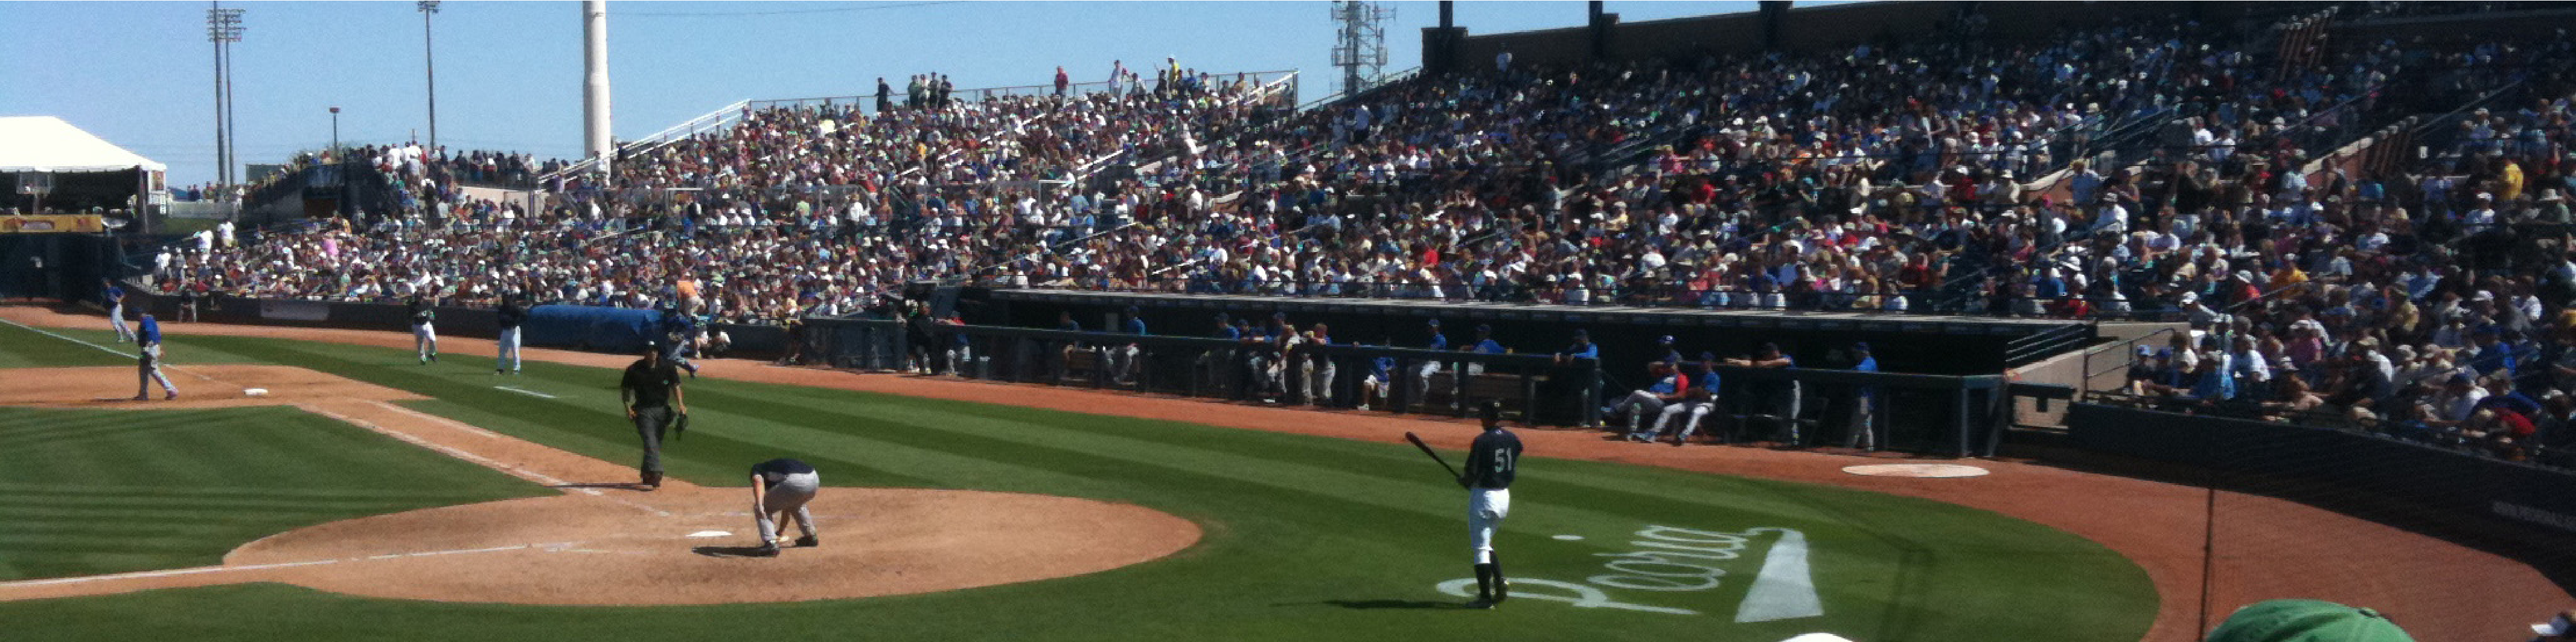
\includegraphics[width=\textwidth]{sampleteaser}
%   \caption{Seattle Mariners at Spring Training, 2010.}
%   \Description{Enjoying the baseball game from the third-base
%     seats. Ichiro Suzuki preparing to bat.}
%   \label{fig:teaser}
% \end{teaserfigure}

%%
%% This command processes the author and affiliation and title
%% information and builds the first part of the formatted document.
\maketitle

\section{Introduction} % Open

Attacks based on combinatorial approaches easily become computationally infeasible because of the vast amount of potential adjacency matrices (\(2^{n^2}\)). With first-order optimization we can approximate the discrete optimization problem. First-order optimization attacks typically require the gradient towards the entries in the adjacency matrix and, hence, reduce the complexity to \(\Theta(n^2)\). To attack a small dataset such as PubMed (19717 nodes), typically more than 20~GB are required if using a dense adjacency matrix. We argue that such memory requirements are still impractical and hinder practitioners to assess adversarial robustness. We identify the necessity to research scalable attacks for GNNs, due to the lack of such attacks for real-world graphs

We propose two strategies how one may apply first-order optimization, without the burden of a dense adjacency matrix. In Section~\ref{sec:attackkdd} we propose an attack that adds adversarial nodes and was one of the top 5 attacks of the KDD Cup 2020~\citep{Biendata2020}. Thereafter in Section~\ref{sec:prbcd}, we describe how one might add/remove edges between existing nodes based on Randomized Block Coordinate Descent (R-BCD). Even though our attacks can be generalized to graph classification, we focus on the important task of node classification.

In this work, we set the foundation for the study of adversarial robustness of GNNs on real-world citation/social networks. Importantly, it is unknown how the adversarial robustness/vulnerability relates to the graph size. In our experiments (Section~\ref{sec:empirical}), we point out that a GNN applied to a larger graph is more fragile w.r.t.\ structure perturbations.

Our contributions are the following:
\begin{itemize}
  \item We show that the widely used cross entropy is not a good surrogate loss for attacking the graph structure on graph neural networks.
  \item We propose a novel loss for global attacks on graph neural networks that overcomes the limitations and empirically boosts the attack strength by up to 100\%.
  \item We propose two scalable adversarial attacks that add/remove edges between the existing nodes. One relies on projected gradient descent and the other uses a greedy FGSM-like optimization scheme (space complexity of \(\Theta(m)\) in the number of edges \(m\)).
  \item We propose one scalable adversarial attack that adds adversarial nodes (space complexity of \(\Theta(n)\)).
  \item We propose a differentiable robust aggregation that scales linearity w.r.t.\ the neighborhood size of the message passing aggregation and performs au par to the previous defense. This enables us to defend a GNN when memory is at premium.
  \item We study the adversarial robustness on graphs substantially larger than PubMed. Empirically, we find that the graph size negatively related to the adversarial robustness.
\end{itemize}

\section{Related Work}\label{sec:related} % Simon

\begin{algorithm}[b]
  \small
  \caption{R-BCD~\citep{Nesterov2012}}
  \label{algo:rbcd}
  \begin{algorithmic}[1]
    \STATE Choose \(\vx_0 \in \R^d\)
    \FOR{\(k \in \{1,2, \dots, K\}\)}
    \STATE Draw random indices \(\vi_k \in \{0, 1, \dots, n\}^b\)
    \STATE \(\vx_{k} \leftarrow \vx_{k-1} - \alpha_{k} \nabla_{\vi_{k}} \mathcal{L}(\vx_{k-1})\)
    \ENDFOR
  \end{algorithmic}
\end{algorithm}

\textbf{Large scale optimization.} In a big data setting, the cost to calculate the gradient towards all variables can be prohibitively high. For this reason, coordinate descent has gained importance in machine learning and large scale optimization~\citep{Wright2015}. \citet{Nesterov2012} proposed (and analyzed the convergence) of Randomized Block Coordinate Descent (R-BCD). For R-BCD's pseudo code see Algorithm~\ref{algo:rbcd}. In R-BCD only a subset of variables is optimized at a time and, hence, only the gradients towards those variables are required. In many cases, this allows for a lower memory footprint and in some settings even converges faster than standard methods~\citep{Nesterov2017}. Constrained optimization with first-order methods can be solved with methods such as Projected Gradient Descent (PGD) or Fast Gradient Sign Method (FGSM)~\cite{Goodfellow2015}. Similarly, one can extend R-BCD to constrained optimization~\citep{Nesterov2012}.

\textbf{Adversarial attacks.} Beginning with~\citep{Dai2018, Zugner2018}, many adversarial attacks on the graph structure have been proposed~\citep{Zugner2019a, Xu2019a, Bojchevski2019, Wu2019, Wang2019, Tang2020}. We limit the scope to an adversary with perfect knowledge about the graph, GNN and test labels. Even this white-box scenario has not been studied for large graphs and our primary goal is to asses adversarial robustness.
%We will consider more sophisticated threat models in future work.
\citet{Dai2018} scale their reinforcement learning approach to a very sparse, large-scale graph for financial transactions. In contrast to our work, they only use a very small budget \(\Delta\) (their time complexity scales linearly with \(\Delta\)). \citet{Wang2019} also scale their attack to a larger graph than PubMed but they do not attack GNNs. \todo{Adversarial attack on large scale graph} analyze adversarial attacks on mini-batch techniques such as Cluster-GCN~\todo{cite}. However, they only scale to a dataset with around 200k nodes and also only consider a local attack. We scale to much bigger datasets, consider a wider class of Graph Neural Networks and also propose a global attack that is scalable. \todo{Mention Fake Node Attacks} propose an attack based on GANs that inserts fake nodes and is the closest related work to our attack in Section~\ref{sec:attackkdd}.

\todo{MGA: Momentum Gradient Attack on Network} First-order optimization attacks such as Metattack~\citep{Zugner2019a} or integrated gradients~\citep{Wu2019} rely on the gradient towards all possible entries in the \textit{dense} adjacency matrix \(\adj\) (quadratic space complexity) to solve the optimization problem for structure perturbations:
\begin{equation}\label{eq:attack}
  \max_{\adj} \mathcal{L}(f_{\theta}(\adj, \features))
\end{equation}
with the adjacency matrix \(\adj\), node features \(\features\), loss \(\mathcal{L}\), and the trained network \(f_{\theta}\).

\todo{defenses}

\section{Cross Entropy is a Bad Surrogate}\label{sec:related} % Simon

In the context of images, typically a single sample is attacked. In the context of graph neural networks this corresponds to a local attack). For such a scenario an untargeted attack may simply maximize the cross entropy \(\text{CE}(y, \vp) = \sum_{c \in \sC} \mathbb{I}[y = c] \log(\evp_{c})\). Many \emph{global} attacks~\citet{Chen2018, Wu2019, Xu2018, Zugner2019a} also attack via maximizing the cross entropy \(\max_{\adj} \text{CE}(f_{\theta}(\adj, \features))\). In our preliminary experiments while attacking a GNN on large graphs, we have often observed that the loss increased while the accuracy increased to.

\begin{proof}
  We are given a graph neural network \(f_{\theta}(\adj, \features)\) with fixed parameters \(\theta\) and want to \(\max_{\adj} \text{CE}(f_{\theta}(\adj, \features))\) s.t.\ the number of edges flipped in \(\adj\) is limited by \(\Delta\). The gradient with softmax activation \(\vp = \text{Softmax}(\vz)\) is given by \(\nicefrac{\partial \text{CE}}{\partial \vz}\)
\end{proof}

Despite its wide use, the surrogate loss cross entropy can be completely uncorrelated with the accuracy if the budget \(\Delta\) of flipping edges is limited. %In contrast, in the traditional (semi-) supervised learning task the budget is only limited via sharing parameters over all samples and regularization.
The cross entropy is unbounded and if the probability of the correct class \(\evp_{c^*}\) approaches 0 it diverges (i.e.\ \(\lim_{p_{c^*} \to 0} \text{CE} = \infty\)). Hence, for small enough budgets \(\Delta\) on a large graph it is possible that the attack only focuses on nodes that are \emph{already wrongly classified} before the attack has even started (for those nodes the gradient is the largest).

A global structure attack has to 1) keep house with the budget \(\Delta\) and 2) find edges that degrade the accuracy maximally. Thus, we propose the subsequent axioms a well-suited, monotonically decreasing surrogate loss \(\mathcal{L^*}(y, \vp)\) should obey for attacking a node-classification algorithm. We define the classification margin as \(\psi = \min_{c \,\text{s.t.}\, c \ne c^*} \evp_{c^*} - \evp{c}\).
\begin{axiom}\label{axiom:axiom1}
  The loss \(\mathcal{L^*}(y, \vp)\) should saturate for low confidence values of the correct class: \(\lim_{\psi \to -1^+} \mathcal{L}(y, \vp) = k < \infty\).
\end{axiom}
\begin{axiom}\label{axiom:axiom2}
  The loss should favour points close to the decision boundary: \(\nicefrac{\partial \mathcal{L}(y, \vp)}{\partial \evp_{c^*}} |_{\psi = 1}  > \nicefrac{\partial \mathcal{L}(y, \vp)}{\partial \evp_{c^*}} |_{\psi \to 0^+}\).
\end{axiom}
Please note that also the widely used margin loss \(\min(0, \psi)\) violates Axiom 2, since all correctly classified nodes receive exactly the same gradient. Obviously, for very low budgets \(\Delta\), it likely better to focus on nodes close to the decision boundary.

One natural choice that fulfills those axioms is the masked cross entropy
\begin{equation}\label{eq:mce}
  \text{MCE} = \frac{1}{|\sV^+|} \sum_{n \in \sV^+} \sum_{c \in \sC} \mathbb{I}[y = c] \log(\evp_{c})
\end{equation}
where \(\sV^+\) is the set of correctly classified nodes. Axiom 1 holds since for a negative margin \(\psi < 0\) the node will be simply omitted. Axiom 2 holds since the gradient \(\nicefrac{\partial \text{MCE}}{\partial \evp_{c^*}}\) is strictly decreasing w.r.t.\ \(\psi\). This loss is well suited for greedy attacks.

However, \(\text{MCE}\) is not a good choice for a projected gradient descent method like the one we are going to propose in Section~\ref{sec:prbcd}. For such an optimization, we typically tune the learning rate such that the budget \(\Delta\) is exceeded after each gradient update and then the project operation maps the parameters back into the feasible region. If we now set the loss to zero / mask it out if wrongly classified, the contributing edges will not gain anything in the gradient update and likely loose strength in the upcoming project step. Hence, those nodes will oscillate at the decision boundary. Therefore, we use tanh of the classification margin
\begin{equation}\label{eq:mce}
  \tanh\text{Margin} = \frac{1}{|\sV|} \sum_{n \in \sV} \tanh(\psi)
\end{equation}
where \(\psi\) denotes the classification margin. This loss obviously fulfills both axioms.

Obviously, one could construct more complicated loss functions considering the asymmetry between correctly and wrongly classified nodes. However, in our experiments we did not achieve much better results. Please note that the reformulations already comes with a significant boost in attack strength.

\todo{Table comparing naive and new loss}

\section{Adding and Removing Edges}\label{sec:prbcd}

In this section we discuss the case where the attack vector is to perturb the existing, binary graph structure:
%
\begin{equation}\label{eq:pgd}
  \max_{\mP\,\,\text{s.t.}\, \sum \mP \le \Delta} \mathcal{L}(f_{\theta}(\adj \oplus \mP, \features))\,.
\end{equation}
%
Here, \(\oplus\) stands for an element-wise exclusive or and \(\Delta\) denotes the edge budget (i.e.\ the number of altered entries in the perturbed adjacency matrix). In the following, we use set \(\sP\) and matrix notation \(\mP\) for the sparse perturbations \(\sP\) interchangeably. Naively, applying R-BCD to optimize towards the dense adjacency matrix would only save some computation on obtaining the respective gradient, but still has a space complexity of \(\mathcal{O}(n^2)\). Note that in R-BCD we interpret each possible entry in the perturbation set \(\sP\) as one dimension of our optimization problem. To mitigate the quadratic complexity, we make use of the fact that the solution is going to be sparse (\(L_0\) perturbation). As in evolutionary algorithms, in each epoch, we keep that part of the search space which is promising and resample the rest. We can view the underlying problem as a combination of \(L_0\)-norm PGD and an adaptive version of Randomized Block Coordinate Descent (R-BCD). R-BCD comes with a space complexity of \(\Theta(m)\), as we typically choose \(\Delta\) to be a fraction of \(m\). We give a formal definition of Projected and Randomized Block Coordinate Descent (PR-BCD) in Algorithm~\ref{algo:prbcd}.

As proposed by~\citet{Xu2019a}, \(\vp\) is interpreted as the probability mass for each potential entry in the perturbation set \(\sP\) and is used in the end to sample the final edge additions/removals. In each epoch \(e \in \{1,2, \dots, E\}\), this probability mass \(\vp\) is used as edge weight. The projection \(\Pi_{\E[\text{Bernoulli}(\vp)] = \Delta} (\vp)\) adjusts the probability mass such that \(\E[\text{Bernoulli}(\vp)] = \sum_{i \in b} \evp_i \approx \Delta\) and that \(\vp \in [0, 1]\) (line 8). If using an undirected graph, the potential edges are restricted to the the upper/lower triangular \(n \times n\) matrix. In the end we sample \(\sP \sim \text{Bernoulli}(\vp)\) (line 16).

Note that the projection of the perturbation set \(\Pi_{\E[\text{Bernoulli}(\vp)] = \Delta} (\vp)\) contains many zero elements, but is not guaranteed to be sparse. If \(\vp\) has more than 50\% non-zero entries, we remove the entries with the lowest probability mass such that 50\% of the search space is resampled. Otherwise, we resample all zero entries in \(\vp\). However, one also might apply a more sophisticated heuristic \(h(\vp)\) (see line 11).

With growing \(n\) it is unrealistic that each possible entry of the adjacency matrix was part of at least one random search space of R-BCD. Apparently, with a constant search space size, the number of mutually exclusive chunks of the perturbation set grows with \(\Theta(n^2)\) and this would imply a quadratic runtime. However, as evident in randomized black-box attacks~\citep{Waniek2018}, it is not necessary to test every possible edge to obtain an effective attack. In Fig.~\ref{fig:randomblocksizeinfluence}, we analyze the influence of the random block size on the perturbed accuracy. For a sufficient block size \(b\) our method performs comparably to its dense equivalent.

We keep the random block fixed and run \(K_{\text{resample}}\) epochs. Thereafter, we decay the learning rate as in~\cite{Xu2019a}. We also employ early stopping for both stages (\(k \le K_{\text{resample}} \text{ and } k > K_{\text{resample}}\) with the epoch \(k\)) such that we take the result of the epoch with highest loss \(\mathcal{L}\).


\begin{figure}[t]
  \centering
  \vspace{-15pt} \resizebox{\linewidth}{!}{%% Creator: Matplotlib, PGF backend
%%
%% To include the figure in your LaTeX document, write
%%   \input{<filename>.pgf}
%%
%% Make sure the required packages are loaded in your preamble
%%   \usepackage{pgf}
%%
%% and, on pdftex
%%   \usepackage[utf8]{inputenc}\DeclareUnicodeCharacter{2212}{-}
%%
%% or, on luatex and xetex
%%   \usepackage{unicode-math}
%%
%% Figures using additional raster images can only be included by \input if
%% they are in the same directory as the main LaTeX file. For loading figures
%% from other directories you can use the `import` package
%%   \usepackage{import}
%%
%% and then include the figures with
%%   \import{<path to file>}{<filename>.pgf}
%%
%% Matplotlib used the following preamble
%%   \usepackage[utf8]{inputenc}
%%   \usepackage[T1]{fontenc}
%%   \usepackage{amsmath}
%%   \newcommand*{\mat}[1]{\boldsymbol{#1}}
%%
\begingroup%
\makeatletter%
\begin{pgfpicture}%
\pgfpathrectangle{\pgfpointorigin}{\pgfqpoint{3.937196in}{0.388266in}}%
\pgfusepath{use as bounding box, clip}%
\begin{pgfscope}%
\pgfsetbuttcap%
\pgfsetmiterjoin%
\definecolor{currentfill}{rgb}{1.000000,1.000000,1.000000}%
\pgfsetfillcolor{currentfill}%
\pgfsetlinewidth{0.000000pt}%
\definecolor{currentstroke}{rgb}{1.000000,1.000000,1.000000}%
\pgfsetstrokecolor{currentstroke}%
\pgfsetstrokeopacity{0.000000}%
\pgfsetdash{}{0pt}%
\pgfpathmoveto{\pgfqpoint{0.000000in}{0.000000in}}%
\pgfpathlineto{\pgfqpoint{3.937196in}{0.000000in}}%
\pgfpathlineto{\pgfqpoint{3.937196in}{0.388266in}}%
\pgfpathlineto{\pgfqpoint{0.000000in}{0.388266in}}%
\pgfpathclose%
\pgfusepath{fill}%
\end{pgfscope}%
\begin{pgfscope}%
\pgfsetbuttcap%
\pgfsetmiterjoin%
\definecolor{currentfill}{rgb}{1.000000,1.000000,1.000000}%
\pgfsetfillcolor{currentfill}%
\pgfsetfillopacity{0.800000}%
\pgfsetlinewidth{1.003750pt}%
\definecolor{currentstroke}{rgb}{0.800000,0.800000,0.800000}%
\pgfsetstrokecolor{currentstroke}%
\pgfsetstrokeopacity{0.800000}%
\pgfsetdash{}{0pt}%
\pgfpathmoveto{\pgfqpoint{0.122222in}{0.100000in}}%
\pgfpathlineto{\pgfqpoint{3.814974in}{0.100000in}}%
\pgfpathquadraticcurveto{\pgfqpoint{3.837196in}{0.100000in}}{\pgfqpoint{3.837196in}{0.122222in}}%
\pgfpathlineto{\pgfqpoint{3.837196in}{0.266044in}}%
\pgfpathquadraticcurveto{\pgfqpoint{3.837196in}{0.288266in}}{\pgfqpoint{3.814974in}{0.288266in}}%
\pgfpathlineto{\pgfqpoint{0.122222in}{0.288266in}}%
\pgfpathquadraticcurveto{\pgfqpoint{0.100000in}{0.288266in}}{\pgfqpoint{0.100000in}{0.266044in}}%
\pgfpathlineto{\pgfqpoint{0.100000in}{0.122222in}}%
\pgfpathquadraticcurveto{\pgfqpoint{0.100000in}{0.100000in}}{\pgfqpoint{0.122222in}{0.100000in}}%
\pgfpathclose%
\pgfusepath{stroke,fill}%
\end{pgfscope}%
\begin{pgfscope}%
\pgfsetbuttcap%
\pgfsetroundjoin%
\pgfsetlinewidth{1.003750pt}%
\definecolor{currentstroke}{rgb}{0.298039,0.447059,0.690196}%
\pgfsetstrokecolor{currentstroke}%
\pgfsetdash{}{0pt}%
\pgfpathmoveto{\pgfqpoint{0.255556in}{0.149378in}}%
\pgfpathlineto{\pgfqpoint{0.255556in}{0.260489in}}%
\pgfusepath{stroke}%
\end{pgfscope}%
\begin{pgfscope}%
\pgfsetroundcap%
\pgfsetroundjoin%
\pgfsetlinewidth{1.003750pt}%
\definecolor{currentstroke}{rgb}{0.298039,0.447059,0.690196}%
\pgfsetstrokecolor{currentstroke}%
\pgfsetdash{}{0pt}%
\pgfpathmoveto{\pgfqpoint{0.144444in}{0.204933in}}%
\pgfpathlineto{\pgfqpoint{0.366667in}{0.204933in}}%
\pgfusepath{stroke}%
\end{pgfscope}%
\begin{pgfscope}%
\definecolor{textcolor}{rgb}{0.150000,0.150000,0.150000}%
\pgfsetstrokecolor{textcolor}%
\pgfsetfillcolor{textcolor}%
\pgftext[x=0.455556in,y=0.166044in,left,base]{\color{textcolor}\rmfamily\fontsize{8.000000}{9.600000}\selectfont Vanilla GCN}%
\end{pgfscope}%
\begin{pgfscope}%
\pgfsetbuttcap%
\pgfsetroundjoin%
\pgfsetlinewidth{1.003750pt}%
\definecolor{currentstroke}{rgb}{0.866667,0.517647,0.321569}%
\pgfsetstrokecolor{currentstroke}%
\pgfsetdash{}{0pt}%
\pgfpathmoveto{\pgfqpoint{1.454988in}{0.149378in}}%
\pgfpathlineto{\pgfqpoint{1.454988in}{0.260489in}}%
\pgfusepath{stroke}%
\end{pgfscope}%
\begin{pgfscope}%
\pgfsetroundcap%
\pgfsetroundjoin%
\pgfsetlinewidth{1.003750pt}%
\definecolor{currentstroke}{rgb}{0.866667,0.517647,0.321569}%
\pgfsetstrokecolor{currentstroke}%
\pgfsetdash{}{0pt}%
\pgfpathmoveto{\pgfqpoint{1.343877in}{0.204933in}}%
\pgfpathlineto{\pgfqpoint{1.566099in}{0.204933in}}%
\pgfusepath{stroke}%
\end{pgfscope}%
\begin{pgfscope}%
\definecolor{textcolor}{rgb}{0.150000,0.150000,0.150000}%
\pgfsetstrokecolor{textcolor}%
\pgfsetfillcolor{textcolor}%
\pgftext[x=1.654988in,y=0.166044in,left,base]{\color{textcolor}\rmfamily\fontsize{8.000000}{9.600000}\selectfont Vanilla GDC}%
\end{pgfscope}%
\begin{pgfscope}%
\pgfsetbuttcap%
\pgfsetroundjoin%
\pgfsetlinewidth{1.003750pt}%
\definecolor{currentstroke}{rgb}{0.333333,0.658824,0.407843}%
\pgfsetstrokecolor{currentstroke}%
\pgfsetdash{}{0pt}%
\pgfpathmoveto{\pgfqpoint{2.656117in}{0.149378in}}%
\pgfpathlineto{\pgfqpoint{2.656117in}{0.260489in}}%
\pgfusepath{stroke}%
\end{pgfscope}%
\begin{pgfscope}%
\pgfsetroundcap%
\pgfsetroundjoin%
\pgfsetlinewidth{1.003750pt}%
\definecolor{currentstroke}{rgb}{0.333333,0.658824,0.407843}%
\pgfsetstrokecolor{currentstroke}%
\pgfsetdash{}{0pt}%
\pgfpathmoveto{\pgfqpoint{2.545006in}{0.204933in}}%
\pgfpathlineto{\pgfqpoint{2.767228in}{0.204933in}}%
\pgfusepath{stroke}%
\end{pgfscope}%
\begin{pgfscope}%
\definecolor{textcolor}{rgb}{0.150000,0.150000,0.150000}%
\pgfsetstrokecolor{textcolor}%
\pgfsetfillcolor{textcolor}%
\pgftext[x=2.856117in,y=0.166044in,left,base]{\color{textcolor}\rmfamily\fontsize{8.000000}{9.600000}\selectfont Soft Median GDC}%
\end{pgfscope}%
\end{pgfpicture}%
\makeatother%
\endgroup%
}
  \makebox[\linewidth][c]{
    \(\begin{array}{cc}
      \subfloat[]{\resizebox{0.5\linewidth}{!}{%% Creator: Matplotlib, PGF backend
%%
%% To include the figure in your LaTeX document, write
%%   \input{<filename>.pgf}
%%
%% Make sure the required packages are loaded in your preamble
%%   \usepackage{pgf}
%%
%% and, on pdftex
%%   \usepackage[utf8]{inputenc}\DeclareUnicodeCharacter{2212}{-}
%%
%% or, on luatex and xetex
%%   \usepackage{unicode-math}
%%
%% Figures using additional raster images can only be included by \input if
%% they are in the same directory as the main LaTeX file. For loading figures
%% from other directories you can use the `import` package
%%   \usepackage{import}
%%
%% and then include the figures with
%%   \import{<path to file>}{<filename>.pgf}
%%
%% Matplotlib used the following preamble
%%   \usepackage[utf8]{inputenc}
%%   \usepackage[T1]{fontenc}
%%   \usepackage{amsmath}
%%   \newcommand*{\mat}[1]{\boldsymbol{#1}}
%%
\begingroup%
\makeatletter%
\begin{pgfpicture}%
\pgfpathrectangle{\pgfpointorigin}{\pgfqpoint{1.986956in}{1.814099in}}%
\pgfusepath{use as bounding box, clip}%
\begin{pgfscope}%
\pgfsetbuttcap%
\pgfsetmiterjoin%
\definecolor{currentfill}{rgb}{1.000000,1.000000,1.000000}%
\pgfsetfillcolor{currentfill}%
\pgfsetlinewidth{0.000000pt}%
\definecolor{currentstroke}{rgb}{1.000000,1.000000,1.000000}%
\pgfsetstrokecolor{currentstroke}%
\pgfsetstrokeopacity{0.000000}%
\pgfsetdash{}{0pt}%
\pgfpathmoveto{\pgfqpoint{0.000000in}{0.000000in}}%
\pgfpathlineto{\pgfqpoint{1.986956in}{0.000000in}}%
\pgfpathlineto{\pgfqpoint{1.986956in}{1.814099in}}%
\pgfpathlineto{\pgfqpoint{0.000000in}{1.814099in}}%
\pgfpathclose%
\pgfusepath{fill}%
\end{pgfscope}%
\begin{pgfscope}%
\pgfsetbuttcap%
\pgfsetmiterjoin%
\definecolor{currentfill}{rgb}{1.000000,1.000000,1.000000}%
\pgfsetfillcolor{currentfill}%
\pgfsetlinewidth{0.000000pt}%
\definecolor{currentstroke}{rgb}{0.000000,0.000000,0.000000}%
\pgfsetstrokecolor{currentstroke}%
\pgfsetstrokeopacity{0.000000}%
\pgfsetdash{}{0pt}%
\pgfpathmoveto{\pgfqpoint{0.578368in}{0.468349in}}%
\pgfpathlineto{\pgfqpoint{1.857118in}{0.468349in}}%
\pgfpathlineto{\pgfqpoint{1.857118in}{1.714099in}}%
\pgfpathlineto{\pgfqpoint{0.578368in}{1.714099in}}%
\pgfpathclose%
\pgfusepath{fill}%
\end{pgfscope}%
\begin{pgfscope}%
\pgfpathrectangle{\pgfqpoint{0.578368in}{0.468349in}}{\pgfqpoint{1.278750in}{1.245750in}}%
\pgfusepath{clip}%
\pgfsetroundcap%
\pgfsetroundjoin%
\pgfsetlinewidth{0.501875pt}%
\definecolor{currentstroke}{rgb}{0.800000,0.800000,0.800000}%
\pgfsetstrokecolor{currentstroke}%
\pgfsetdash{}{0pt}%
\pgfpathmoveto{\pgfqpoint{0.742505in}{0.468349in}}%
\pgfpathlineto{\pgfqpoint{0.742505in}{1.714099in}}%
\pgfusepath{stroke}%
\end{pgfscope}%
\begin{pgfscope}%
\definecolor{textcolor}{rgb}{0.150000,0.150000,0.150000}%
\pgfsetstrokecolor{textcolor}%
\pgfsetfillcolor{textcolor}%
\pgftext[x=0.742505in,y=0.378072in,,top]{\color{textcolor}\rmfamily\fontsize{8.000000}{9.600000}\selectfont \(\displaystyle {10^{4}}\)}%
\end{pgfscope}%
\begin{pgfscope}%
\pgfpathrectangle{\pgfqpoint{0.578368in}{0.468349in}}{\pgfqpoint{1.278750in}{1.245750in}}%
\pgfusepath{clip}%
\pgfsetroundcap%
\pgfsetroundjoin%
\pgfsetlinewidth{0.501875pt}%
\definecolor{currentstroke}{rgb}{0.800000,0.800000,0.800000}%
\pgfsetstrokecolor{currentstroke}%
\pgfsetdash{}{0pt}%
\pgfpathmoveto{\pgfqpoint{1.094667in}{0.468349in}}%
\pgfpathlineto{\pgfqpoint{1.094667in}{1.714099in}}%
\pgfusepath{stroke}%
\end{pgfscope}%
\begin{pgfscope}%
\definecolor{textcolor}{rgb}{0.150000,0.150000,0.150000}%
\pgfsetstrokecolor{textcolor}%
\pgfsetfillcolor{textcolor}%
\pgftext[x=1.094667in,y=0.378072in,,top]{\color{textcolor}\rmfamily\fontsize{8.000000}{9.600000}\selectfont \(\displaystyle {10^{5}}\)}%
\end{pgfscope}%
\begin{pgfscope}%
\pgfpathrectangle{\pgfqpoint{0.578368in}{0.468349in}}{\pgfqpoint{1.278750in}{1.245750in}}%
\pgfusepath{clip}%
\pgfsetroundcap%
\pgfsetroundjoin%
\pgfsetlinewidth{0.501875pt}%
\definecolor{currentstroke}{rgb}{0.800000,0.800000,0.800000}%
\pgfsetstrokecolor{currentstroke}%
\pgfsetdash{}{0pt}%
\pgfpathmoveto{\pgfqpoint{1.446830in}{0.468349in}}%
\pgfpathlineto{\pgfqpoint{1.446830in}{1.714099in}}%
\pgfusepath{stroke}%
\end{pgfscope}%
\begin{pgfscope}%
\definecolor{textcolor}{rgb}{0.150000,0.150000,0.150000}%
\pgfsetstrokecolor{textcolor}%
\pgfsetfillcolor{textcolor}%
\pgftext[x=1.446830in,y=0.378072in,,top]{\color{textcolor}\rmfamily\fontsize{8.000000}{9.600000}\selectfont \(\displaystyle {10^{6}}\)}%
\end{pgfscope}%
\begin{pgfscope}%
\pgfpathrectangle{\pgfqpoint{0.578368in}{0.468349in}}{\pgfqpoint{1.278750in}{1.245750in}}%
\pgfusepath{clip}%
\pgfsetroundcap%
\pgfsetroundjoin%
\pgfsetlinewidth{0.501875pt}%
\definecolor{currentstroke}{rgb}{0.800000,0.800000,0.800000}%
\pgfsetstrokecolor{currentstroke}%
\pgfsetdash{}{0pt}%
\pgfpathmoveto{\pgfqpoint{1.798993in}{0.468349in}}%
\pgfpathlineto{\pgfqpoint{1.798993in}{1.714099in}}%
\pgfusepath{stroke}%
\end{pgfscope}%
\begin{pgfscope}%
\definecolor{textcolor}{rgb}{0.150000,0.150000,0.150000}%
\pgfsetstrokecolor{textcolor}%
\pgfsetfillcolor{textcolor}%
\pgftext[x=1.798993in,y=0.378072in,,top]{\color{textcolor}\rmfamily\fontsize{8.000000}{9.600000}\selectfont \(\displaystyle {10^{7}}\)}%
\end{pgfscope}%
\begin{pgfscope}%
\definecolor{textcolor}{rgb}{0.150000,0.150000,0.150000}%
\pgfsetstrokecolor{textcolor}%
\pgfsetfillcolor{textcolor}%
\pgftext[x=1.217743in,y=0.222655in,,top]{\color{textcolor}\rmfamily\fontsize{10.000000}{12.000000}\selectfont Block size \(\displaystyle b\)}%
\end{pgfscope}%
\begin{pgfscope}%
\pgfpathrectangle{\pgfqpoint{0.578368in}{0.468349in}}{\pgfqpoint{1.278750in}{1.245750in}}%
\pgfusepath{clip}%
\pgfsetroundcap%
\pgfsetroundjoin%
\pgfsetlinewidth{0.501875pt}%
\definecolor{currentstroke}{rgb}{0.800000,0.800000,0.800000}%
\pgfsetstrokecolor{currentstroke}%
\pgfsetdash{}{0pt}%
\pgfpathmoveto{\pgfqpoint{0.578368in}{0.781918in}}%
\pgfpathlineto{\pgfqpoint{1.857118in}{0.781918in}}%
\pgfusepath{stroke}%
\end{pgfscope}%
\begin{pgfscope}%
\definecolor{textcolor}{rgb}{0.150000,0.150000,0.150000}%
\pgfsetstrokecolor{textcolor}%
\pgfsetfillcolor{textcolor}%
\pgftext[x=0.278211in, y=0.743656in, left, base]{\color{textcolor}\rmfamily\fontsize{8.000000}{9.600000}\selectfont \(\displaystyle {0.65}\)}%
\end{pgfscope}%
\begin{pgfscope}%
\pgfpathrectangle{\pgfqpoint{0.578368in}{0.468349in}}{\pgfqpoint{1.278750in}{1.245750in}}%
\pgfusepath{clip}%
\pgfsetroundcap%
\pgfsetroundjoin%
\pgfsetlinewidth{0.501875pt}%
\definecolor{currentstroke}{rgb}{0.800000,0.800000,0.800000}%
\pgfsetstrokecolor{currentstroke}%
\pgfsetdash{}{0pt}%
\pgfpathmoveto{\pgfqpoint{0.578368in}{1.196101in}}%
\pgfpathlineto{\pgfqpoint{1.857118in}{1.196101in}}%
\pgfusepath{stroke}%
\end{pgfscope}%
\begin{pgfscope}%
\definecolor{textcolor}{rgb}{0.150000,0.150000,0.150000}%
\pgfsetstrokecolor{textcolor}%
\pgfsetfillcolor{textcolor}%
\pgftext[x=0.278211in, y=1.157839in, left, base]{\color{textcolor}\rmfamily\fontsize{8.000000}{9.600000}\selectfont \(\displaystyle {0.70}\)}%
\end{pgfscope}%
\begin{pgfscope}%
\pgfpathrectangle{\pgfqpoint{0.578368in}{0.468349in}}{\pgfqpoint{1.278750in}{1.245750in}}%
\pgfusepath{clip}%
\pgfsetroundcap%
\pgfsetroundjoin%
\pgfsetlinewidth{0.501875pt}%
\definecolor{currentstroke}{rgb}{0.800000,0.800000,0.800000}%
\pgfsetstrokecolor{currentstroke}%
\pgfsetdash{}{0pt}%
\pgfpathmoveto{\pgfqpoint{0.578368in}{1.610284in}}%
\pgfpathlineto{\pgfqpoint{1.857118in}{1.610284in}}%
\pgfusepath{stroke}%
\end{pgfscope}%
\begin{pgfscope}%
\definecolor{textcolor}{rgb}{0.150000,0.150000,0.150000}%
\pgfsetstrokecolor{textcolor}%
\pgfsetfillcolor{textcolor}%
\pgftext[x=0.278211in, y=1.572022in, left, base]{\color{textcolor}\rmfamily\fontsize{8.000000}{9.600000}\selectfont \(\displaystyle {0.75}\)}%
\end{pgfscope}%
\begin{pgfscope}%
\definecolor{textcolor}{rgb}{0.150000,0.150000,0.150000}%
\pgfsetstrokecolor{textcolor}%
\pgfsetfillcolor{textcolor}%
\pgftext[x=0.222655in,y=1.091224in,,bottom,rotate=90.000000]{\color{textcolor}\rmfamily\fontsize{10.000000}{12.000000}\selectfont Accuracy}%
\end{pgfscope}%
\begin{pgfscope}%
\pgfpathrectangle{\pgfqpoint{0.578368in}{0.468349in}}{\pgfqpoint{1.278750in}{1.245750in}}%
\pgfusepath{clip}%
\pgfsetbuttcap%
\pgfsetroundjoin%
\pgfsetlinewidth{1.003750pt}%
\definecolor{currentstroke}{rgb}{0.298039,0.447059,0.690196}%
\pgfsetstrokecolor{currentstroke}%
\pgfsetdash{}{0pt}%
\pgfpathmoveto{\pgfqpoint{0.636493in}{0.625052in}}%
\pgfpathlineto{\pgfqpoint{0.636493in}{0.640835in}}%
\pgfusepath{stroke}%
\end{pgfscope}%
\begin{pgfscope}%
\pgfpathrectangle{\pgfqpoint{0.578368in}{0.468349in}}{\pgfqpoint{1.278750in}{1.245750in}}%
\pgfusepath{clip}%
\pgfsetbuttcap%
\pgfsetroundjoin%
\pgfsetlinewidth{1.003750pt}%
\definecolor{currentstroke}{rgb}{0.298039,0.447059,0.690196}%
\pgfsetstrokecolor{currentstroke}%
\pgfsetdash{}{0pt}%
\pgfpathmoveto{\pgfqpoint{0.742505in}{0.625052in}}%
\pgfpathlineto{\pgfqpoint{0.742505in}{0.640835in}}%
\pgfusepath{stroke}%
\end{pgfscope}%
\begin{pgfscope}%
\pgfpathrectangle{\pgfqpoint{0.578368in}{0.468349in}}{\pgfqpoint{1.278750in}{1.245750in}}%
\pgfusepath{clip}%
\pgfsetbuttcap%
\pgfsetroundjoin%
\pgfsetlinewidth{1.003750pt}%
\definecolor{currentstroke}{rgb}{0.298039,0.447059,0.690196}%
\pgfsetstrokecolor{currentstroke}%
\pgfsetdash{}{0pt}%
\pgfpathmoveto{\pgfqpoint{1.094667in}{0.625052in}}%
\pgfpathlineto{\pgfqpoint{1.094667in}{0.640835in}}%
\pgfusepath{stroke}%
\end{pgfscope}%
\begin{pgfscope}%
\pgfpathrectangle{\pgfqpoint{0.578368in}{0.468349in}}{\pgfqpoint{1.278750in}{1.245750in}}%
\pgfusepath{clip}%
\pgfsetbuttcap%
\pgfsetroundjoin%
\pgfsetlinewidth{1.003750pt}%
\definecolor{currentstroke}{rgb}{0.298039,0.447059,0.690196}%
\pgfsetstrokecolor{currentstroke}%
\pgfsetdash{}{0pt}%
\pgfpathmoveto{\pgfqpoint{1.446830in}{0.625052in}}%
\pgfpathlineto{\pgfqpoint{1.446830in}{0.640835in}}%
\pgfusepath{stroke}%
\end{pgfscope}%
\begin{pgfscope}%
\pgfpathrectangle{\pgfqpoint{0.578368in}{0.468349in}}{\pgfqpoint{1.278750in}{1.245750in}}%
\pgfusepath{clip}%
\pgfsetbuttcap%
\pgfsetroundjoin%
\pgfsetlinewidth{1.003750pt}%
\definecolor{currentstroke}{rgb}{0.298039,0.447059,0.690196}%
\pgfsetstrokecolor{currentstroke}%
\pgfsetdash{}{0pt}%
\pgfpathmoveto{\pgfqpoint{1.798993in}{0.625052in}}%
\pgfpathlineto{\pgfqpoint{1.798993in}{0.640835in}}%
\pgfusepath{stroke}%
\end{pgfscope}%
\begin{pgfscope}%
\pgfpathrectangle{\pgfqpoint{0.578368in}{0.468349in}}{\pgfqpoint{1.278750in}{1.245750in}}%
\pgfusepath{clip}%
\pgfsetbuttcap%
\pgfsetroundjoin%
\pgfsetlinewidth{1.003750pt}%
\definecolor{currentstroke}{rgb}{0.866667,0.517647,0.321569}%
\pgfsetstrokecolor{currentstroke}%
\pgfsetdash{}{0pt}%
\pgfpathmoveto{\pgfqpoint{0.636493in}{0.764691in}}%
\pgfpathlineto{\pgfqpoint{0.636493in}{0.781465in}}%
\pgfusepath{stroke}%
\end{pgfscope}%
\begin{pgfscope}%
\pgfpathrectangle{\pgfqpoint{0.578368in}{0.468349in}}{\pgfqpoint{1.278750in}{1.245750in}}%
\pgfusepath{clip}%
\pgfsetbuttcap%
\pgfsetroundjoin%
\pgfsetlinewidth{1.003750pt}%
\definecolor{currentstroke}{rgb}{0.866667,0.517647,0.321569}%
\pgfsetstrokecolor{currentstroke}%
\pgfsetdash{}{0pt}%
\pgfpathmoveto{\pgfqpoint{0.742505in}{0.764691in}}%
\pgfpathlineto{\pgfqpoint{0.742505in}{0.781465in}}%
\pgfusepath{stroke}%
\end{pgfscope}%
\begin{pgfscope}%
\pgfpathrectangle{\pgfqpoint{0.578368in}{0.468349in}}{\pgfqpoint{1.278750in}{1.245750in}}%
\pgfusepath{clip}%
\pgfsetbuttcap%
\pgfsetroundjoin%
\pgfsetlinewidth{1.003750pt}%
\definecolor{currentstroke}{rgb}{0.866667,0.517647,0.321569}%
\pgfsetstrokecolor{currentstroke}%
\pgfsetdash{}{0pt}%
\pgfpathmoveto{\pgfqpoint{1.094667in}{0.764691in}}%
\pgfpathlineto{\pgfqpoint{1.094667in}{0.781465in}}%
\pgfusepath{stroke}%
\end{pgfscope}%
\begin{pgfscope}%
\pgfpathrectangle{\pgfqpoint{0.578368in}{0.468349in}}{\pgfqpoint{1.278750in}{1.245750in}}%
\pgfusepath{clip}%
\pgfsetbuttcap%
\pgfsetroundjoin%
\pgfsetlinewidth{1.003750pt}%
\definecolor{currentstroke}{rgb}{0.866667,0.517647,0.321569}%
\pgfsetstrokecolor{currentstroke}%
\pgfsetdash{}{0pt}%
\pgfpathmoveto{\pgfqpoint{1.446830in}{0.764691in}}%
\pgfpathlineto{\pgfqpoint{1.446830in}{0.781465in}}%
\pgfusepath{stroke}%
\end{pgfscope}%
\begin{pgfscope}%
\pgfpathrectangle{\pgfqpoint{0.578368in}{0.468349in}}{\pgfqpoint{1.278750in}{1.245750in}}%
\pgfusepath{clip}%
\pgfsetbuttcap%
\pgfsetroundjoin%
\pgfsetlinewidth{1.003750pt}%
\definecolor{currentstroke}{rgb}{0.866667,0.517647,0.321569}%
\pgfsetstrokecolor{currentstroke}%
\pgfsetdash{}{0pt}%
\pgfpathmoveto{\pgfqpoint{1.798993in}{0.764691in}}%
\pgfpathlineto{\pgfqpoint{1.798993in}{0.781465in}}%
\pgfusepath{stroke}%
\end{pgfscope}%
\begin{pgfscope}%
\pgfpathrectangle{\pgfqpoint{0.578368in}{0.468349in}}{\pgfqpoint{1.278750in}{1.245750in}}%
\pgfusepath{clip}%
\pgfsetbuttcap%
\pgfsetroundjoin%
\pgfsetlinewidth{1.003750pt}%
\definecolor{currentstroke}{rgb}{0.333333,0.658824,0.407843}%
\pgfsetstrokecolor{currentstroke}%
\pgfsetdash{}{0pt}%
\pgfpathmoveto{\pgfqpoint{0.636493in}{1.608289in}}%
\pgfpathlineto{\pgfqpoint{0.636493in}{1.644366in}}%
\pgfusepath{stroke}%
\end{pgfscope}%
\begin{pgfscope}%
\pgfpathrectangle{\pgfqpoint{0.578368in}{0.468349in}}{\pgfqpoint{1.278750in}{1.245750in}}%
\pgfusepath{clip}%
\pgfsetbuttcap%
\pgfsetroundjoin%
\pgfsetlinewidth{1.003750pt}%
\definecolor{currentstroke}{rgb}{0.333333,0.658824,0.407843}%
\pgfsetstrokecolor{currentstroke}%
\pgfsetdash{}{0pt}%
\pgfpathmoveto{\pgfqpoint{0.742505in}{1.608289in}}%
\pgfpathlineto{\pgfqpoint{0.742505in}{1.644366in}}%
\pgfusepath{stroke}%
\end{pgfscope}%
\begin{pgfscope}%
\pgfpathrectangle{\pgfqpoint{0.578368in}{0.468349in}}{\pgfqpoint{1.278750in}{1.245750in}}%
\pgfusepath{clip}%
\pgfsetbuttcap%
\pgfsetroundjoin%
\pgfsetlinewidth{1.003750pt}%
\definecolor{currentstroke}{rgb}{0.333333,0.658824,0.407843}%
\pgfsetstrokecolor{currentstroke}%
\pgfsetdash{}{0pt}%
\pgfpathmoveto{\pgfqpoint{1.094667in}{1.608289in}}%
\pgfpathlineto{\pgfqpoint{1.094667in}{1.644366in}}%
\pgfusepath{stroke}%
\end{pgfscope}%
\begin{pgfscope}%
\pgfpathrectangle{\pgfqpoint{0.578368in}{0.468349in}}{\pgfqpoint{1.278750in}{1.245750in}}%
\pgfusepath{clip}%
\pgfsetbuttcap%
\pgfsetroundjoin%
\pgfsetlinewidth{1.003750pt}%
\definecolor{currentstroke}{rgb}{0.333333,0.658824,0.407843}%
\pgfsetstrokecolor{currentstroke}%
\pgfsetdash{}{0pt}%
\pgfpathmoveto{\pgfqpoint{1.446830in}{1.608289in}}%
\pgfpathlineto{\pgfqpoint{1.446830in}{1.644366in}}%
\pgfusepath{stroke}%
\end{pgfscope}%
\begin{pgfscope}%
\pgfpathrectangle{\pgfqpoint{0.578368in}{0.468349in}}{\pgfqpoint{1.278750in}{1.245750in}}%
\pgfusepath{clip}%
\pgfsetbuttcap%
\pgfsetroundjoin%
\pgfsetlinewidth{1.003750pt}%
\definecolor{currentstroke}{rgb}{0.333333,0.658824,0.407843}%
\pgfsetstrokecolor{currentstroke}%
\pgfsetdash{}{0pt}%
\pgfpathmoveto{\pgfqpoint{1.798993in}{1.608289in}}%
\pgfpathlineto{\pgfqpoint{1.798993in}{1.644366in}}%
\pgfusepath{stroke}%
\end{pgfscope}%
\begin{pgfscope}%
\pgfpathrectangle{\pgfqpoint{0.578368in}{0.468349in}}{\pgfqpoint{1.278750in}{1.245750in}}%
\pgfusepath{clip}%
\pgfsetbuttcap%
\pgfsetroundjoin%
\pgfsetlinewidth{1.003750pt}%
\definecolor{currentstroke}{rgb}{0.298039,0.447059,0.690196}%
\pgfsetstrokecolor{currentstroke}%
\pgfsetdash{}{0pt}%
\pgfpathmoveto{\pgfqpoint{0.636493in}{0.538067in}}%
\pgfpathlineto{\pgfqpoint{0.636493in}{0.667575in}}%
\pgfusepath{stroke}%
\end{pgfscope}%
\begin{pgfscope}%
\pgfpathrectangle{\pgfqpoint{0.578368in}{0.468349in}}{\pgfqpoint{1.278750in}{1.245750in}}%
\pgfusepath{clip}%
\pgfsetbuttcap%
\pgfsetroundjoin%
\pgfsetlinewidth{1.003750pt}%
\definecolor{currentstroke}{rgb}{0.298039,0.447059,0.690196}%
\pgfsetstrokecolor{currentstroke}%
\pgfsetdash{}{0pt}%
\pgfpathmoveto{\pgfqpoint{0.742505in}{0.524974in}}%
\pgfpathlineto{\pgfqpoint{0.742505in}{0.647926in}}%
\pgfusepath{stroke}%
\end{pgfscope}%
\begin{pgfscope}%
\pgfpathrectangle{\pgfqpoint{0.578368in}{0.468349in}}{\pgfqpoint{1.278750in}{1.245750in}}%
\pgfusepath{clip}%
\pgfsetbuttcap%
\pgfsetroundjoin%
\pgfsetlinewidth{1.003750pt}%
\definecolor{currentstroke}{rgb}{0.298039,0.447059,0.690196}%
\pgfsetstrokecolor{currentstroke}%
\pgfsetdash{}{0pt}%
\pgfpathmoveto{\pgfqpoint{1.094667in}{0.597287in}}%
\pgfpathlineto{\pgfqpoint{1.094667in}{0.707890in}}%
\pgfusepath{stroke}%
\end{pgfscope}%
\begin{pgfscope}%
\pgfpathrectangle{\pgfqpoint{0.578368in}{0.468349in}}{\pgfqpoint{1.278750in}{1.245750in}}%
\pgfusepath{clip}%
\pgfsetbuttcap%
\pgfsetroundjoin%
\pgfsetlinewidth{1.003750pt}%
\definecolor{currentstroke}{rgb}{0.298039,0.447059,0.690196}%
\pgfsetstrokecolor{currentstroke}%
\pgfsetdash{}{0pt}%
\pgfpathmoveto{\pgfqpoint{1.446830in}{0.638855in}}%
\pgfpathlineto{\pgfqpoint{1.446830in}{0.740973in}}%
\pgfusepath{stroke}%
\end{pgfscope}%
\begin{pgfscope}%
\pgfpathrectangle{\pgfqpoint{0.578368in}{0.468349in}}{\pgfqpoint{1.278750in}{1.245750in}}%
\pgfusepath{clip}%
\pgfsetbuttcap%
\pgfsetroundjoin%
\pgfsetlinewidth{1.003750pt}%
\definecolor{currentstroke}{rgb}{0.298039,0.447059,0.690196}%
\pgfsetstrokecolor{currentstroke}%
\pgfsetdash{}{0pt}%
\pgfpathmoveto{\pgfqpoint{1.798993in}{0.614827in}}%
\pgfpathlineto{\pgfqpoint{1.798993in}{0.719163in}}%
\pgfusepath{stroke}%
\end{pgfscope}%
\begin{pgfscope}%
\pgfpathrectangle{\pgfqpoint{0.578368in}{0.468349in}}{\pgfqpoint{1.278750in}{1.245750in}}%
\pgfusepath{clip}%
\pgfsetbuttcap%
\pgfsetroundjoin%
\pgfsetlinewidth{1.003750pt}%
\definecolor{currentstroke}{rgb}{0.866667,0.517647,0.321569}%
\pgfsetstrokecolor{currentstroke}%
\pgfsetdash{}{0pt}%
\pgfpathmoveto{\pgfqpoint{0.636493in}{0.691867in}}%
\pgfpathlineto{\pgfqpoint{0.636493in}{0.742967in}}%
\pgfusepath{stroke}%
\end{pgfscope}%
\begin{pgfscope}%
\pgfpathrectangle{\pgfqpoint{0.578368in}{0.468349in}}{\pgfqpoint{1.278750in}{1.245750in}}%
\pgfusepath{clip}%
\pgfsetbuttcap%
\pgfsetroundjoin%
\pgfsetlinewidth{1.003750pt}%
\definecolor{currentstroke}{rgb}{0.866667,0.517647,0.321569}%
\pgfsetstrokecolor{currentstroke}%
\pgfsetdash{}{0pt}%
\pgfpathmoveto{\pgfqpoint{0.742505in}{0.675290in}}%
\pgfpathlineto{\pgfqpoint{0.742505in}{0.734660in}}%
\pgfusepath{stroke}%
\end{pgfscope}%
\begin{pgfscope}%
\pgfpathrectangle{\pgfqpoint{0.578368in}{0.468349in}}{\pgfqpoint{1.278750in}{1.245750in}}%
\pgfusepath{clip}%
\pgfsetbuttcap%
\pgfsetroundjoin%
\pgfsetlinewidth{1.003750pt}%
\definecolor{currentstroke}{rgb}{0.866667,0.517647,0.321569}%
\pgfsetstrokecolor{currentstroke}%
\pgfsetdash{}{0pt}%
\pgfpathmoveto{\pgfqpoint{1.094667in}{0.775110in}}%
\pgfpathlineto{\pgfqpoint{1.094667in}{0.829982in}}%
\pgfusepath{stroke}%
\end{pgfscope}%
\begin{pgfscope}%
\pgfpathrectangle{\pgfqpoint{0.578368in}{0.468349in}}{\pgfqpoint{1.278750in}{1.245750in}}%
\pgfusepath{clip}%
\pgfsetbuttcap%
\pgfsetroundjoin%
\pgfsetlinewidth{1.003750pt}%
\definecolor{currentstroke}{rgb}{0.866667,0.517647,0.321569}%
\pgfsetstrokecolor{currentstroke}%
\pgfsetdash{}{0pt}%
\pgfpathmoveto{\pgfqpoint{1.446830in}{0.802791in}}%
\pgfpathlineto{\pgfqpoint{1.446830in}{0.850758in}}%
\pgfusepath{stroke}%
\end{pgfscope}%
\begin{pgfscope}%
\pgfpathrectangle{\pgfqpoint{0.578368in}{0.468349in}}{\pgfqpoint{1.278750in}{1.245750in}}%
\pgfusepath{clip}%
\pgfsetbuttcap%
\pgfsetroundjoin%
\pgfsetlinewidth{1.003750pt}%
\definecolor{currentstroke}{rgb}{0.866667,0.517647,0.321569}%
\pgfsetstrokecolor{currentstroke}%
\pgfsetdash{}{0pt}%
\pgfpathmoveto{\pgfqpoint{1.798993in}{0.774780in}}%
\pgfpathlineto{\pgfqpoint{1.798993in}{0.819834in}}%
\pgfusepath{stroke}%
\end{pgfscope}%
\begin{pgfscope}%
\pgfpathrectangle{\pgfqpoint{0.578368in}{0.468349in}}{\pgfqpoint{1.278750in}{1.245750in}}%
\pgfusepath{clip}%
\pgfsetbuttcap%
\pgfsetroundjoin%
\pgfsetlinewidth{1.003750pt}%
\definecolor{currentstroke}{rgb}{0.333333,0.658824,0.407843}%
\pgfsetstrokecolor{currentstroke}%
\pgfsetdash{}{0pt}%
\pgfpathmoveto{\pgfqpoint{0.636493in}{1.552231in}}%
\pgfpathlineto{\pgfqpoint{0.636493in}{1.629703in}}%
\pgfusepath{stroke}%
\end{pgfscope}%
\begin{pgfscope}%
\pgfpathrectangle{\pgfqpoint{0.578368in}{0.468349in}}{\pgfqpoint{1.278750in}{1.245750in}}%
\pgfusepath{clip}%
\pgfsetbuttcap%
\pgfsetroundjoin%
\pgfsetlinewidth{1.003750pt}%
\definecolor{currentstroke}{rgb}{0.333333,0.658824,0.407843}%
\pgfsetstrokecolor{currentstroke}%
\pgfsetdash{}{0pt}%
\pgfpathmoveto{\pgfqpoint{0.742505in}{1.547155in}}%
\pgfpathlineto{\pgfqpoint{0.742505in}{1.628230in}}%
\pgfusepath{stroke}%
\end{pgfscope}%
\begin{pgfscope}%
\pgfpathrectangle{\pgfqpoint{0.578368in}{0.468349in}}{\pgfqpoint{1.278750in}{1.245750in}}%
\pgfusepath{clip}%
\pgfsetbuttcap%
\pgfsetroundjoin%
\pgfsetlinewidth{1.003750pt}%
\definecolor{currentstroke}{rgb}{0.333333,0.658824,0.407843}%
\pgfsetstrokecolor{currentstroke}%
\pgfsetdash{}{0pt}%
\pgfpathmoveto{\pgfqpoint{1.094667in}{1.601729in}}%
\pgfpathlineto{\pgfqpoint{1.094667in}{1.657474in}}%
\pgfusepath{stroke}%
\end{pgfscope}%
\begin{pgfscope}%
\pgfpathrectangle{\pgfqpoint{0.578368in}{0.468349in}}{\pgfqpoint{1.278750in}{1.245750in}}%
\pgfusepath{clip}%
\pgfsetbuttcap%
\pgfsetroundjoin%
\pgfsetlinewidth{1.003750pt}%
\definecolor{currentstroke}{rgb}{0.333333,0.658824,0.407843}%
\pgfsetstrokecolor{currentstroke}%
\pgfsetdash{}{0pt}%
\pgfpathmoveto{\pgfqpoint{1.446830in}{1.554634in}}%
\pgfpathlineto{\pgfqpoint{1.446830in}{1.643015in}}%
\pgfusepath{stroke}%
\end{pgfscope}%
\begin{pgfscope}%
\pgfpathrectangle{\pgfqpoint{0.578368in}{0.468349in}}{\pgfqpoint{1.278750in}{1.245750in}}%
\pgfusepath{clip}%
\pgfsetbuttcap%
\pgfsetroundjoin%
\pgfsetlinewidth{1.003750pt}%
\definecolor{currentstroke}{rgb}{0.333333,0.658824,0.407843}%
\pgfsetstrokecolor{currentstroke}%
\pgfsetdash{}{0pt}%
\pgfpathmoveto{\pgfqpoint{1.798993in}{1.598360in}}%
\pgfpathlineto{\pgfqpoint{1.798993in}{1.650366in}}%
\pgfusepath{stroke}%
\end{pgfscope}%
\begin{pgfscope}%
\pgfpathrectangle{\pgfqpoint{0.578368in}{0.468349in}}{\pgfqpoint{1.278750in}{1.245750in}}%
\pgfusepath{clip}%
\pgfsetbuttcap%
\pgfsetroundjoin%
\pgfsetlinewidth{1.003750pt}%
\definecolor{currentstroke}{rgb}{0.298039,0.447059,0.690196}%
\pgfsetstrokecolor{currentstroke}%
\pgfsetdash{{6.400000pt}{1.600000pt}{1.000000pt}{1.600000pt}}{0.000000pt}%
\pgfpathmoveto{\pgfqpoint{0.636493in}{0.632943in}}%
\pgfpathlineto{\pgfqpoint{0.742505in}{0.632943in}}%
\pgfpathlineto{\pgfqpoint{1.094667in}{0.632943in}}%
\pgfpathlineto{\pgfqpoint{1.446830in}{0.632943in}}%
\pgfpathlineto{\pgfqpoint{1.798993in}{0.632943in}}%
\pgfusepath{stroke}%
\end{pgfscope}%
\begin{pgfscope}%
\pgfpathrectangle{\pgfqpoint{0.578368in}{0.468349in}}{\pgfqpoint{1.278750in}{1.245750in}}%
\pgfusepath{clip}%
\pgfsetbuttcap%
\pgfsetroundjoin%
\pgfsetlinewidth{1.003750pt}%
\definecolor{currentstroke}{rgb}{0.866667,0.517647,0.321569}%
\pgfsetstrokecolor{currentstroke}%
\pgfsetdash{{6.400000pt}{1.600000pt}{1.000000pt}{1.600000pt}}{0.000000pt}%
\pgfpathmoveto{\pgfqpoint{0.636493in}{0.773078in}}%
\pgfpathlineto{\pgfqpoint{0.742505in}{0.773078in}}%
\pgfpathlineto{\pgfqpoint{1.094667in}{0.773078in}}%
\pgfpathlineto{\pgfqpoint{1.446830in}{0.773078in}}%
\pgfpathlineto{\pgfqpoint{1.798993in}{0.773078in}}%
\pgfusepath{stroke}%
\end{pgfscope}%
\begin{pgfscope}%
\pgfpathrectangle{\pgfqpoint{0.578368in}{0.468349in}}{\pgfqpoint{1.278750in}{1.245750in}}%
\pgfusepath{clip}%
\pgfsetbuttcap%
\pgfsetroundjoin%
\pgfsetlinewidth{1.003750pt}%
\definecolor{currentstroke}{rgb}{0.333333,0.658824,0.407843}%
\pgfsetstrokecolor{currentstroke}%
\pgfsetdash{{6.400000pt}{1.600000pt}{1.000000pt}{1.600000pt}}{0.000000pt}%
\pgfpathmoveto{\pgfqpoint{0.636493in}{1.626328in}}%
\pgfpathlineto{\pgfqpoint{0.742505in}{1.626328in}}%
\pgfpathlineto{\pgfqpoint{1.094667in}{1.626328in}}%
\pgfpathlineto{\pgfqpoint{1.446830in}{1.626328in}}%
\pgfpathlineto{\pgfqpoint{1.798993in}{1.626328in}}%
\pgfusepath{stroke}%
\end{pgfscope}%
\begin{pgfscope}%
\pgfpathrectangle{\pgfqpoint{0.578368in}{0.468349in}}{\pgfqpoint{1.278750in}{1.245750in}}%
\pgfusepath{clip}%
\pgfsetroundcap%
\pgfsetroundjoin%
\pgfsetlinewidth{1.003750pt}%
\definecolor{currentstroke}{rgb}{0.298039,0.447059,0.690196}%
\pgfsetstrokecolor{currentstroke}%
\pgfsetdash{}{0pt}%
\pgfpathmoveto{\pgfqpoint{0.636493in}{0.602821in}}%
\pgfpathlineto{\pgfqpoint{0.742505in}{0.586450in}}%
\pgfpathlineto{\pgfqpoint{1.094667in}{0.652589in}}%
\pgfpathlineto{\pgfqpoint{1.446830in}{0.689914in}}%
\pgfpathlineto{\pgfqpoint{1.798993in}{0.666995in}}%
\pgfusepath{stroke}%
\end{pgfscope}%
\begin{pgfscope}%
\pgfpathrectangle{\pgfqpoint{0.578368in}{0.468349in}}{\pgfqpoint{1.278750in}{1.245750in}}%
\pgfusepath{clip}%
\pgfsetroundcap%
\pgfsetroundjoin%
\pgfsetlinewidth{1.003750pt}%
\definecolor{currentstroke}{rgb}{0.866667,0.517647,0.321569}%
\pgfsetstrokecolor{currentstroke}%
\pgfsetdash{}{0pt}%
\pgfpathmoveto{\pgfqpoint{0.636493in}{0.717417in}}%
\pgfpathlineto{\pgfqpoint{0.742505in}{0.704975in}}%
\pgfpathlineto{\pgfqpoint{1.094667in}{0.802546in}}%
\pgfpathlineto{\pgfqpoint{1.446830in}{0.826775in}}%
\pgfpathlineto{\pgfqpoint{1.798993in}{0.797307in}}%
\pgfusepath{stroke}%
\end{pgfscope}%
\begin{pgfscope}%
\pgfpathrectangle{\pgfqpoint{0.578368in}{0.468349in}}{\pgfqpoint{1.278750in}{1.245750in}}%
\pgfusepath{clip}%
\pgfsetroundcap%
\pgfsetroundjoin%
\pgfsetlinewidth{1.003750pt}%
\definecolor{currentstroke}{rgb}{0.333333,0.658824,0.407843}%
\pgfsetstrokecolor{currentstroke}%
\pgfsetdash{}{0pt}%
\pgfpathmoveto{\pgfqpoint{0.636493in}{1.590967in}}%
\pgfpathlineto{\pgfqpoint{0.742505in}{1.587693in}}%
\pgfpathlineto{\pgfqpoint{1.094667in}{1.629602in}}%
\pgfpathlineto{\pgfqpoint{1.446830in}{1.598825in}}%
\pgfpathlineto{\pgfqpoint{1.798993in}{1.624363in}}%
\pgfusepath{stroke}%
\end{pgfscope}%
\begin{pgfscope}%
\pgfsetrectcap%
\pgfsetmiterjoin%
\pgfsetlinewidth{0.752812pt}%
\definecolor{currentstroke}{rgb}{0.700000,0.700000,0.700000}%
\pgfsetstrokecolor{currentstroke}%
\pgfsetdash{}{0pt}%
\pgfpathmoveto{\pgfqpoint{0.578368in}{0.468349in}}%
\pgfpathlineto{\pgfqpoint{0.578368in}{1.714099in}}%
\pgfusepath{stroke}%
\end{pgfscope}%
\begin{pgfscope}%
\pgfsetrectcap%
\pgfsetmiterjoin%
\pgfsetlinewidth{0.752812pt}%
\definecolor{currentstroke}{rgb}{0.700000,0.700000,0.700000}%
\pgfsetstrokecolor{currentstroke}%
\pgfsetdash{}{0pt}%
\pgfpathmoveto{\pgfqpoint{1.857118in}{0.468349in}}%
\pgfpathlineto{\pgfqpoint{1.857118in}{1.714099in}}%
\pgfusepath{stroke}%
\end{pgfscope}%
\begin{pgfscope}%
\pgfsetrectcap%
\pgfsetmiterjoin%
\pgfsetlinewidth{0.752812pt}%
\definecolor{currentstroke}{rgb}{0.700000,0.700000,0.700000}%
\pgfsetstrokecolor{currentstroke}%
\pgfsetdash{}{0pt}%
\pgfpathmoveto{\pgfqpoint{0.578368in}{0.468349in}}%
\pgfpathlineto{\pgfqpoint{1.857118in}{0.468349in}}%
\pgfusepath{stroke}%
\end{pgfscope}%
\begin{pgfscope}%
\pgfsetrectcap%
\pgfsetmiterjoin%
\pgfsetlinewidth{0.752812pt}%
\definecolor{currentstroke}{rgb}{0.700000,0.700000,0.700000}%
\pgfsetstrokecolor{currentstroke}%
\pgfsetdash{}{0pt}%
\pgfpathmoveto{\pgfqpoint{0.578368in}{1.714099in}}%
\pgfpathlineto{\pgfqpoint{1.857118in}{1.714099in}}%
\pgfusepath{stroke}%
\end{pgfscope}%
\end{pgfpicture}%
\makeatother%
\endgroup%
}} &
      \subfloat[]{\resizebox{0.5\linewidth}{!}{%% Creator: Matplotlib, PGF backend
%%
%% To include the figure in your LaTeX document, write
%%   \input{<filename>.pgf}
%%
%% Make sure the required packages are loaded in your preamble
%%   \usepackage{pgf}
%%
%% and, on pdftex
%%   \usepackage[utf8]{inputenc}\DeclareUnicodeCharacter{2212}{-}
%%
%% or, on luatex and xetex
%%   \usepackage{unicode-math}
%%
%% Figures using additional raster images can only be included by \input if
%% they are in the same directory as the main LaTeX file. For loading figures
%% from other directories you can use the `import` package
%%   \usepackage{import}
%%
%% and then include the figures with
%%   \import{<path to file>}{<filename>.pgf}
%%
%% Matplotlib used the following preamble
%%   \usepackage[utf8]{inputenc}
%%   \usepackage[T1]{fontenc}
%%   \usepackage{amsmath}
%%   \newcommand*{\mat}[1]{\boldsymbol{#1}}
%%
\begingroup%
\makeatletter%
\begin{pgfpicture}%
\pgfpathrectangle{\pgfpointorigin}{\pgfqpoint{1.927928in}{1.814099in}}%
\pgfusepath{use as bounding box, clip}%
\begin{pgfscope}%
\pgfsetbuttcap%
\pgfsetmiterjoin%
\definecolor{currentfill}{rgb}{1.000000,1.000000,1.000000}%
\pgfsetfillcolor{currentfill}%
\pgfsetlinewidth{0.000000pt}%
\definecolor{currentstroke}{rgb}{1.000000,1.000000,1.000000}%
\pgfsetstrokecolor{currentstroke}%
\pgfsetstrokeopacity{0.000000}%
\pgfsetdash{}{0pt}%
\pgfpathmoveto{\pgfqpoint{0.000000in}{0.000000in}}%
\pgfpathlineto{\pgfqpoint{1.927928in}{0.000000in}}%
\pgfpathlineto{\pgfqpoint{1.927928in}{1.814099in}}%
\pgfpathlineto{\pgfqpoint{0.000000in}{1.814099in}}%
\pgfpathclose%
\pgfusepath{fill}%
\end{pgfscope}%
\begin{pgfscope}%
\pgfsetbuttcap%
\pgfsetmiterjoin%
\definecolor{currentfill}{rgb}{1.000000,1.000000,1.000000}%
\pgfsetfillcolor{currentfill}%
\pgfsetlinewidth{0.000000pt}%
\definecolor{currentstroke}{rgb}{0.000000,0.000000,0.000000}%
\pgfsetstrokecolor{currentstroke}%
\pgfsetstrokeopacity{0.000000}%
\pgfsetdash{}{0pt}%
\pgfpathmoveto{\pgfqpoint{0.519339in}{0.468349in}}%
\pgfpathlineto{\pgfqpoint{1.798089in}{0.468349in}}%
\pgfpathlineto{\pgfqpoint{1.798089in}{1.714099in}}%
\pgfpathlineto{\pgfqpoint{0.519339in}{1.714099in}}%
\pgfpathclose%
\pgfusepath{fill}%
\end{pgfscope}%
\begin{pgfscope}%
\pgfpathrectangle{\pgfqpoint{0.519339in}{0.468349in}}{\pgfqpoint{1.278750in}{1.245750in}}%
\pgfusepath{clip}%
\pgfsetroundcap%
\pgfsetroundjoin%
\pgfsetlinewidth{0.501875pt}%
\definecolor{currentstroke}{rgb}{0.800000,0.800000,0.800000}%
\pgfsetstrokecolor{currentstroke}%
\pgfsetdash{}{0pt}%
\pgfpathmoveto{\pgfqpoint{0.683476in}{0.468349in}}%
\pgfpathlineto{\pgfqpoint{0.683476in}{1.714099in}}%
\pgfusepath{stroke}%
\end{pgfscope}%
\begin{pgfscope}%
\definecolor{textcolor}{rgb}{0.150000,0.150000,0.150000}%
\pgfsetstrokecolor{textcolor}%
\pgfsetfillcolor{textcolor}%
\pgftext[x=0.683476in,y=0.378072in,,top]{\color{textcolor}\rmfamily\fontsize{8.000000}{9.600000}\selectfont \(\displaystyle {10^{4}}\)}%
\end{pgfscope}%
\begin{pgfscope}%
\pgfpathrectangle{\pgfqpoint{0.519339in}{0.468349in}}{\pgfqpoint{1.278750in}{1.245750in}}%
\pgfusepath{clip}%
\pgfsetroundcap%
\pgfsetroundjoin%
\pgfsetlinewidth{0.501875pt}%
\definecolor{currentstroke}{rgb}{0.800000,0.800000,0.800000}%
\pgfsetstrokecolor{currentstroke}%
\pgfsetdash{}{0pt}%
\pgfpathmoveto{\pgfqpoint{1.035639in}{0.468349in}}%
\pgfpathlineto{\pgfqpoint{1.035639in}{1.714099in}}%
\pgfusepath{stroke}%
\end{pgfscope}%
\begin{pgfscope}%
\definecolor{textcolor}{rgb}{0.150000,0.150000,0.150000}%
\pgfsetstrokecolor{textcolor}%
\pgfsetfillcolor{textcolor}%
\pgftext[x=1.035639in,y=0.378072in,,top]{\color{textcolor}\rmfamily\fontsize{8.000000}{9.600000}\selectfont \(\displaystyle {10^{5}}\)}%
\end{pgfscope}%
\begin{pgfscope}%
\pgfpathrectangle{\pgfqpoint{0.519339in}{0.468349in}}{\pgfqpoint{1.278750in}{1.245750in}}%
\pgfusepath{clip}%
\pgfsetroundcap%
\pgfsetroundjoin%
\pgfsetlinewidth{0.501875pt}%
\definecolor{currentstroke}{rgb}{0.800000,0.800000,0.800000}%
\pgfsetstrokecolor{currentstroke}%
\pgfsetdash{}{0pt}%
\pgfpathmoveto{\pgfqpoint{1.387802in}{0.468349in}}%
\pgfpathlineto{\pgfqpoint{1.387802in}{1.714099in}}%
\pgfusepath{stroke}%
\end{pgfscope}%
\begin{pgfscope}%
\definecolor{textcolor}{rgb}{0.150000,0.150000,0.150000}%
\pgfsetstrokecolor{textcolor}%
\pgfsetfillcolor{textcolor}%
\pgftext[x=1.387802in,y=0.378072in,,top]{\color{textcolor}\rmfamily\fontsize{8.000000}{9.600000}\selectfont \(\displaystyle {10^{6}}\)}%
\end{pgfscope}%
\begin{pgfscope}%
\pgfpathrectangle{\pgfqpoint{0.519339in}{0.468349in}}{\pgfqpoint{1.278750in}{1.245750in}}%
\pgfusepath{clip}%
\pgfsetroundcap%
\pgfsetroundjoin%
\pgfsetlinewidth{0.501875pt}%
\definecolor{currentstroke}{rgb}{0.800000,0.800000,0.800000}%
\pgfsetstrokecolor{currentstroke}%
\pgfsetdash{}{0pt}%
\pgfpathmoveto{\pgfqpoint{1.739964in}{0.468349in}}%
\pgfpathlineto{\pgfqpoint{1.739964in}{1.714099in}}%
\pgfusepath{stroke}%
\end{pgfscope}%
\begin{pgfscope}%
\definecolor{textcolor}{rgb}{0.150000,0.150000,0.150000}%
\pgfsetstrokecolor{textcolor}%
\pgfsetfillcolor{textcolor}%
\pgftext[x=1.739964in,y=0.378072in,,top]{\color{textcolor}\rmfamily\fontsize{8.000000}{9.600000}\selectfont \(\displaystyle {10^{7}}\)}%
\end{pgfscope}%
\begin{pgfscope}%
\definecolor{textcolor}{rgb}{0.150000,0.150000,0.150000}%
\pgfsetstrokecolor{textcolor}%
\pgfsetfillcolor{textcolor}%
\pgftext[x=1.158714in,y=0.222655in,,top]{\color{textcolor}\rmfamily\fontsize{10.000000}{12.000000}\selectfont Block size \(\displaystyle b\)}%
\end{pgfscope}%
\begin{pgfscope}%
\pgfpathrectangle{\pgfqpoint{0.519339in}{0.468349in}}{\pgfqpoint{1.278750in}{1.245750in}}%
\pgfusepath{clip}%
\pgfsetroundcap%
\pgfsetroundjoin%
\pgfsetlinewidth{0.501875pt}%
\definecolor{currentstroke}{rgb}{0.800000,0.800000,0.800000}%
\pgfsetstrokecolor{currentstroke}%
\pgfsetdash{}{0pt}%
\pgfpathmoveto{\pgfqpoint{0.519339in}{0.626756in}}%
\pgfpathlineto{\pgfqpoint{1.798089in}{0.626756in}}%
\pgfusepath{stroke}%
\end{pgfscope}%
\begin{pgfscope}%
\definecolor{textcolor}{rgb}{0.150000,0.150000,0.150000}%
\pgfsetstrokecolor{textcolor}%
\pgfsetfillcolor{textcolor}%
\pgftext[x=0.278211in, y=0.588494in, left, base]{\color{textcolor}\rmfamily\fontsize{8.000000}{9.600000}\selectfont \(\displaystyle {0.5}\)}%
\end{pgfscope}%
\begin{pgfscope}%
\pgfpathrectangle{\pgfqpoint{0.519339in}{0.468349in}}{\pgfqpoint{1.278750in}{1.245750in}}%
\pgfusepath{clip}%
\pgfsetroundcap%
\pgfsetroundjoin%
\pgfsetlinewidth{0.501875pt}%
\definecolor{currentstroke}{rgb}{0.800000,0.800000,0.800000}%
\pgfsetstrokecolor{currentstroke}%
\pgfsetdash{}{0pt}%
\pgfpathmoveto{\pgfqpoint{0.519339in}{1.086245in}}%
\pgfpathlineto{\pgfqpoint{1.798089in}{1.086245in}}%
\pgfusepath{stroke}%
\end{pgfscope}%
\begin{pgfscope}%
\definecolor{textcolor}{rgb}{0.150000,0.150000,0.150000}%
\pgfsetstrokecolor{textcolor}%
\pgfsetfillcolor{textcolor}%
\pgftext[x=0.278211in, y=1.047982in, left, base]{\color{textcolor}\rmfamily\fontsize{8.000000}{9.600000}\selectfont \(\displaystyle {0.6}\)}%
\end{pgfscope}%
\begin{pgfscope}%
\pgfpathrectangle{\pgfqpoint{0.519339in}{0.468349in}}{\pgfqpoint{1.278750in}{1.245750in}}%
\pgfusepath{clip}%
\pgfsetroundcap%
\pgfsetroundjoin%
\pgfsetlinewidth{0.501875pt}%
\definecolor{currentstroke}{rgb}{0.800000,0.800000,0.800000}%
\pgfsetstrokecolor{currentstroke}%
\pgfsetdash{}{0pt}%
\pgfpathmoveto{\pgfqpoint{0.519339in}{1.545733in}}%
\pgfpathlineto{\pgfqpoint{1.798089in}{1.545733in}}%
\pgfusepath{stroke}%
\end{pgfscope}%
\begin{pgfscope}%
\definecolor{textcolor}{rgb}{0.150000,0.150000,0.150000}%
\pgfsetstrokecolor{textcolor}%
\pgfsetfillcolor{textcolor}%
\pgftext[x=0.278211in, y=1.507470in, left, base]{\color{textcolor}\rmfamily\fontsize{8.000000}{9.600000}\selectfont \(\displaystyle {0.7}\)}%
\end{pgfscope}%
\begin{pgfscope}%
\definecolor{textcolor}{rgb}{0.150000,0.150000,0.150000}%
\pgfsetstrokecolor{textcolor}%
\pgfsetfillcolor{textcolor}%
\pgftext[x=0.222655in,y=1.091224in,,bottom,rotate=90.000000]{\color{textcolor}\rmfamily\fontsize{10.000000}{12.000000}\selectfont Accuracy}%
\end{pgfscope}%
\begin{pgfscope}%
\pgfpathrectangle{\pgfqpoint{0.519339in}{0.468349in}}{\pgfqpoint{1.278750in}{1.245750in}}%
\pgfusepath{clip}%
\pgfsetbuttcap%
\pgfsetroundjoin%
\pgfsetlinewidth{1.003750pt}%
\definecolor{currentstroke}{rgb}{0.298039,0.447059,0.690196}%
\pgfsetstrokecolor{currentstroke}%
\pgfsetdash{}{0pt}%
\pgfpathmoveto{\pgfqpoint{0.577464in}{0.572305in}}%
\pgfpathlineto{\pgfqpoint{0.577464in}{0.583861in}}%
\pgfusepath{stroke}%
\end{pgfscope}%
\begin{pgfscope}%
\pgfpathrectangle{\pgfqpoint{0.519339in}{0.468349in}}{\pgfqpoint{1.278750in}{1.245750in}}%
\pgfusepath{clip}%
\pgfsetbuttcap%
\pgfsetroundjoin%
\pgfsetlinewidth{1.003750pt}%
\definecolor{currentstroke}{rgb}{0.298039,0.447059,0.690196}%
\pgfsetstrokecolor{currentstroke}%
\pgfsetdash{}{0pt}%
\pgfpathmoveto{\pgfqpoint{0.683476in}{0.572305in}}%
\pgfpathlineto{\pgfqpoint{0.683476in}{0.583861in}}%
\pgfusepath{stroke}%
\end{pgfscope}%
\begin{pgfscope}%
\pgfpathrectangle{\pgfqpoint{0.519339in}{0.468349in}}{\pgfqpoint{1.278750in}{1.245750in}}%
\pgfusepath{clip}%
\pgfsetbuttcap%
\pgfsetroundjoin%
\pgfsetlinewidth{1.003750pt}%
\definecolor{currentstroke}{rgb}{0.298039,0.447059,0.690196}%
\pgfsetstrokecolor{currentstroke}%
\pgfsetdash{}{0pt}%
\pgfpathmoveto{\pgfqpoint{1.035639in}{0.572305in}}%
\pgfpathlineto{\pgfqpoint{1.035639in}{0.583861in}}%
\pgfusepath{stroke}%
\end{pgfscope}%
\begin{pgfscope}%
\pgfpathrectangle{\pgfqpoint{0.519339in}{0.468349in}}{\pgfqpoint{1.278750in}{1.245750in}}%
\pgfusepath{clip}%
\pgfsetbuttcap%
\pgfsetroundjoin%
\pgfsetlinewidth{1.003750pt}%
\definecolor{currentstroke}{rgb}{0.298039,0.447059,0.690196}%
\pgfsetstrokecolor{currentstroke}%
\pgfsetdash{}{0pt}%
\pgfpathmoveto{\pgfqpoint{1.387802in}{0.572305in}}%
\pgfpathlineto{\pgfqpoint{1.387802in}{0.583861in}}%
\pgfusepath{stroke}%
\end{pgfscope}%
\begin{pgfscope}%
\pgfpathrectangle{\pgfqpoint{0.519339in}{0.468349in}}{\pgfqpoint{1.278750in}{1.245750in}}%
\pgfusepath{clip}%
\pgfsetbuttcap%
\pgfsetroundjoin%
\pgfsetlinewidth{1.003750pt}%
\definecolor{currentstroke}{rgb}{0.298039,0.447059,0.690196}%
\pgfsetstrokecolor{currentstroke}%
\pgfsetdash{}{0pt}%
\pgfpathmoveto{\pgfqpoint{1.739964in}{0.572305in}}%
\pgfpathlineto{\pgfqpoint{1.739964in}{0.583861in}}%
\pgfusepath{stroke}%
\end{pgfscope}%
\begin{pgfscope}%
\pgfpathrectangle{\pgfqpoint{0.519339in}{0.468349in}}{\pgfqpoint{1.278750in}{1.245750in}}%
\pgfusepath{clip}%
\pgfsetbuttcap%
\pgfsetroundjoin%
\pgfsetlinewidth{1.003750pt}%
\definecolor{currentstroke}{rgb}{0.866667,0.517647,0.321569}%
\pgfsetstrokecolor{currentstroke}%
\pgfsetdash{}{0pt}%
\pgfpathmoveto{\pgfqpoint{0.577464in}{0.761593in}}%
\pgfpathlineto{\pgfqpoint{0.577464in}{0.773061in}}%
\pgfusepath{stroke}%
\end{pgfscope}%
\begin{pgfscope}%
\pgfpathrectangle{\pgfqpoint{0.519339in}{0.468349in}}{\pgfqpoint{1.278750in}{1.245750in}}%
\pgfusepath{clip}%
\pgfsetbuttcap%
\pgfsetroundjoin%
\pgfsetlinewidth{1.003750pt}%
\definecolor{currentstroke}{rgb}{0.866667,0.517647,0.321569}%
\pgfsetstrokecolor{currentstroke}%
\pgfsetdash{}{0pt}%
\pgfpathmoveto{\pgfqpoint{0.683476in}{0.761593in}}%
\pgfpathlineto{\pgfqpoint{0.683476in}{0.773061in}}%
\pgfusepath{stroke}%
\end{pgfscope}%
\begin{pgfscope}%
\pgfpathrectangle{\pgfqpoint{0.519339in}{0.468349in}}{\pgfqpoint{1.278750in}{1.245750in}}%
\pgfusepath{clip}%
\pgfsetbuttcap%
\pgfsetroundjoin%
\pgfsetlinewidth{1.003750pt}%
\definecolor{currentstroke}{rgb}{0.866667,0.517647,0.321569}%
\pgfsetstrokecolor{currentstroke}%
\pgfsetdash{}{0pt}%
\pgfpathmoveto{\pgfqpoint{1.035639in}{0.761593in}}%
\pgfpathlineto{\pgfqpoint{1.035639in}{0.773061in}}%
\pgfusepath{stroke}%
\end{pgfscope}%
\begin{pgfscope}%
\pgfpathrectangle{\pgfqpoint{0.519339in}{0.468349in}}{\pgfqpoint{1.278750in}{1.245750in}}%
\pgfusepath{clip}%
\pgfsetbuttcap%
\pgfsetroundjoin%
\pgfsetlinewidth{1.003750pt}%
\definecolor{currentstroke}{rgb}{0.866667,0.517647,0.321569}%
\pgfsetstrokecolor{currentstroke}%
\pgfsetdash{}{0pt}%
\pgfpathmoveto{\pgfqpoint{1.387802in}{0.761593in}}%
\pgfpathlineto{\pgfqpoint{1.387802in}{0.773061in}}%
\pgfusepath{stroke}%
\end{pgfscope}%
\begin{pgfscope}%
\pgfpathrectangle{\pgfqpoint{0.519339in}{0.468349in}}{\pgfqpoint{1.278750in}{1.245750in}}%
\pgfusepath{clip}%
\pgfsetbuttcap%
\pgfsetroundjoin%
\pgfsetlinewidth{1.003750pt}%
\definecolor{currentstroke}{rgb}{0.866667,0.517647,0.321569}%
\pgfsetstrokecolor{currentstroke}%
\pgfsetdash{}{0pt}%
\pgfpathmoveto{\pgfqpoint{1.739964in}{0.761593in}}%
\pgfpathlineto{\pgfqpoint{1.739964in}{0.773061in}}%
\pgfusepath{stroke}%
\end{pgfscope}%
\begin{pgfscope}%
\pgfpathrectangle{\pgfqpoint{0.519339in}{0.468349in}}{\pgfqpoint{1.278750in}{1.245750in}}%
\pgfusepath{clip}%
\pgfsetbuttcap%
\pgfsetroundjoin%
\pgfsetlinewidth{1.003750pt}%
\definecolor{currentstroke}{rgb}{0.333333,0.658824,0.407843}%
\pgfsetstrokecolor{currentstroke}%
\pgfsetdash{}{0pt}%
\pgfpathmoveto{\pgfqpoint{0.577464in}{1.617700in}}%
\pgfpathlineto{\pgfqpoint{0.577464in}{1.643031in}}%
\pgfusepath{stroke}%
\end{pgfscope}%
\begin{pgfscope}%
\pgfpathrectangle{\pgfqpoint{0.519339in}{0.468349in}}{\pgfqpoint{1.278750in}{1.245750in}}%
\pgfusepath{clip}%
\pgfsetbuttcap%
\pgfsetroundjoin%
\pgfsetlinewidth{1.003750pt}%
\definecolor{currentstroke}{rgb}{0.333333,0.658824,0.407843}%
\pgfsetstrokecolor{currentstroke}%
\pgfsetdash{}{0pt}%
\pgfpathmoveto{\pgfqpoint{0.683476in}{1.617700in}}%
\pgfpathlineto{\pgfqpoint{0.683476in}{1.643031in}}%
\pgfusepath{stroke}%
\end{pgfscope}%
\begin{pgfscope}%
\pgfpathrectangle{\pgfqpoint{0.519339in}{0.468349in}}{\pgfqpoint{1.278750in}{1.245750in}}%
\pgfusepath{clip}%
\pgfsetbuttcap%
\pgfsetroundjoin%
\pgfsetlinewidth{1.003750pt}%
\definecolor{currentstroke}{rgb}{0.333333,0.658824,0.407843}%
\pgfsetstrokecolor{currentstroke}%
\pgfsetdash{}{0pt}%
\pgfpathmoveto{\pgfqpoint{1.035639in}{1.617700in}}%
\pgfpathlineto{\pgfqpoint{1.035639in}{1.643031in}}%
\pgfusepath{stroke}%
\end{pgfscope}%
\begin{pgfscope}%
\pgfpathrectangle{\pgfqpoint{0.519339in}{0.468349in}}{\pgfqpoint{1.278750in}{1.245750in}}%
\pgfusepath{clip}%
\pgfsetbuttcap%
\pgfsetroundjoin%
\pgfsetlinewidth{1.003750pt}%
\definecolor{currentstroke}{rgb}{0.333333,0.658824,0.407843}%
\pgfsetstrokecolor{currentstroke}%
\pgfsetdash{}{0pt}%
\pgfpathmoveto{\pgfqpoint{1.387802in}{1.617700in}}%
\pgfpathlineto{\pgfqpoint{1.387802in}{1.643031in}}%
\pgfusepath{stroke}%
\end{pgfscope}%
\begin{pgfscope}%
\pgfpathrectangle{\pgfqpoint{0.519339in}{0.468349in}}{\pgfqpoint{1.278750in}{1.245750in}}%
\pgfusepath{clip}%
\pgfsetbuttcap%
\pgfsetroundjoin%
\pgfsetlinewidth{1.003750pt}%
\definecolor{currentstroke}{rgb}{0.333333,0.658824,0.407843}%
\pgfsetstrokecolor{currentstroke}%
\pgfsetdash{}{0pt}%
\pgfpathmoveto{\pgfqpoint{1.739964in}{1.617700in}}%
\pgfpathlineto{\pgfqpoint{1.739964in}{1.643031in}}%
\pgfusepath{stroke}%
\end{pgfscope}%
\begin{pgfscope}%
\pgfpathrectangle{\pgfqpoint{0.519339in}{0.468349in}}{\pgfqpoint{1.278750in}{1.245750in}}%
\pgfusepath{clip}%
\pgfsetbuttcap%
\pgfsetroundjoin%
\pgfsetlinewidth{1.003750pt}%
\definecolor{currentstroke}{rgb}{0.298039,0.447059,0.690196}%
\pgfsetstrokecolor{currentstroke}%
\pgfsetdash{}{0pt}%
\pgfpathmoveto{\pgfqpoint{0.577464in}{0.861605in}}%
\pgfpathlineto{\pgfqpoint{0.577464in}{0.920046in}}%
\pgfusepath{stroke}%
\end{pgfscope}%
\begin{pgfscope}%
\pgfpathrectangle{\pgfqpoint{0.519339in}{0.468349in}}{\pgfqpoint{1.278750in}{1.245750in}}%
\pgfusepath{clip}%
\pgfsetbuttcap%
\pgfsetroundjoin%
\pgfsetlinewidth{1.003750pt}%
\definecolor{currentstroke}{rgb}{0.298039,0.447059,0.690196}%
\pgfsetstrokecolor{currentstroke}%
\pgfsetdash{}{0pt}%
\pgfpathmoveto{\pgfqpoint{0.683476in}{0.524974in}}%
\pgfpathlineto{\pgfqpoint{0.683476in}{0.596322in}}%
\pgfusepath{stroke}%
\end{pgfscope}%
\begin{pgfscope}%
\pgfpathrectangle{\pgfqpoint{0.519339in}{0.468349in}}{\pgfqpoint{1.278750in}{1.245750in}}%
\pgfusepath{clip}%
\pgfsetbuttcap%
\pgfsetroundjoin%
\pgfsetlinewidth{1.003750pt}%
\definecolor{currentstroke}{rgb}{0.298039,0.447059,0.690196}%
\pgfsetstrokecolor{currentstroke}%
\pgfsetdash{}{0pt}%
\pgfpathmoveto{\pgfqpoint{1.035639in}{0.565227in}}%
\pgfpathlineto{\pgfqpoint{1.035639in}{0.632348in}}%
\pgfusepath{stroke}%
\end{pgfscope}%
\begin{pgfscope}%
\pgfpathrectangle{\pgfqpoint{0.519339in}{0.468349in}}{\pgfqpoint{1.278750in}{1.245750in}}%
\pgfusepath{clip}%
\pgfsetbuttcap%
\pgfsetroundjoin%
\pgfsetlinewidth{1.003750pt}%
\definecolor{currentstroke}{rgb}{0.298039,0.447059,0.690196}%
\pgfsetstrokecolor{currentstroke}%
\pgfsetdash{}{0pt}%
\pgfpathmoveto{\pgfqpoint{1.387802in}{0.576213in}}%
\pgfpathlineto{\pgfqpoint{1.387802in}{0.644609in}}%
\pgfusepath{stroke}%
\end{pgfscope}%
\begin{pgfscope}%
\pgfpathrectangle{\pgfqpoint{0.519339in}{0.468349in}}{\pgfqpoint{1.278750in}{1.245750in}}%
\pgfusepath{clip}%
\pgfsetbuttcap%
\pgfsetroundjoin%
\pgfsetlinewidth{1.003750pt}%
\definecolor{currentstroke}{rgb}{0.298039,0.447059,0.690196}%
\pgfsetstrokecolor{currentstroke}%
\pgfsetdash{}{0pt}%
\pgfpathmoveto{\pgfqpoint{1.739964in}{0.595263in}}%
\pgfpathlineto{\pgfqpoint{1.739964in}{0.674232in}}%
\pgfusepath{stroke}%
\end{pgfscope}%
\begin{pgfscope}%
\pgfpathrectangle{\pgfqpoint{0.519339in}{0.468349in}}{\pgfqpoint{1.278750in}{1.245750in}}%
\pgfusepath{clip}%
\pgfsetbuttcap%
\pgfsetroundjoin%
\pgfsetlinewidth{1.003750pt}%
\definecolor{currentstroke}{rgb}{0.866667,0.517647,0.321569}%
\pgfsetstrokecolor{currentstroke}%
\pgfsetdash{}{0pt}%
\pgfpathmoveto{\pgfqpoint{0.577464in}{0.952718in}}%
\pgfpathlineto{\pgfqpoint{0.577464in}{0.980764in}}%
\pgfusepath{stroke}%
\end{pgfscope}%
\begin{pgfscope}%
\pgfpathrectangle{\pgfqpoint{0.519339in}{0.468349in}}{\pgfqpoint{1.278750in}{1.245750in}}%
\pgfusepath{clip}%
\pgfsetbuttcap%
\pgfsetroundjoin%
\pgfsetlinewidth{1.003750pt}%
\definecolor{currentstroke}{rgb}{0.866667,0.517647,0.321569}%
\pgfsetstrokecolor{currentstroke}%
\pgfsetdash{}{0pt}%
\pgfpathmoveto{\pgfqpoint{0.683476in}{0.675369in}}%
\pgfpathlineto{\pgfqpoint{0.683476in}{0.702369in}}%
\pgfusepath{stroke}%
\end{pgfscope}%
\begin{pgfscope}%
\pgfpathrectangle{\pgfqpoint{0.519339in}{0.468349in}}{\pgfqpoint{1.278750in}{1.245750in}}%
\pgfusepath{clip}%
\pgfsetbuttcap%
\pgfsetroundjoin%
\pgfsetlinewidth{1.003750pt}%
\definecolor{currentstroke}{rgb}{0.866667,0.517647,0.321569}%
\pgfsetstrokecolor{currentstroke}%
\pgfsetdash{}{0pt}%
\pgfpathmoveto{\pgfqpoint{1.035639in}{0.765863in}}%
\pgfpathlineto{\pgfqpoint{1.035639in}{0.806567in}}%
\pgfusepath{stroke}%
\end{pgfscope}%
\begin{pgfscope}%
\pgfpathrectangle{\pgfqpoint{0.519339in}{0.468349in}}{\pgfqpoint{1.278750in}{1.245750in}}%
\pgfusepath{clip}%
\pgfsetbuttcap%
\pgfsetroundjoin%
\pgfsetlinewidth{1.003750pt}%
\definecolor{currentstroke}{rgb}{0.866667,0.517647,0.321569}%
\pgfsetstrokecolor{currentstroke}%
\pgfsetdash{}{0pt}%
\pgfpathmoveto{\pgfqpoint{1.387802in}{0.784254in}}%
\pgfpathlineto{\pgfqpoint{1.387802in}{0.832491in}}%
\pgfusepath{stroke}%
\end{pgfscope}%
\begin{pgfscope}%
\pgfpathrectangle{\pgfqpoint{0.519339in}{0.468349in}}{\pgfqpoint{1.278750in}{1.245750in}}%
\pgfusepath{clip}%
\pgfsetbuttcap%
\pgfsetroundjoin%
\pgfsetlinewidth{1.003750pt}%
\definecolor{currentstroke}{rgb}{0.866667,0.517647,0.321569}%
\pgfsetstrokecolor{currentstroke}%
\pgfsetdash{}{0pt}%
\pgfpathmoveto{\pgfqpoint{1.739964in}{0.818506in}}%
\pgfpathlineto{\pgfqpoint{1.739964in}{0.862894in}}%
\pgfusepath{stroke}%
\end{pgfscope}%
\begin{pgfscope}%
\pgfpathrectangle{\pgfqpoint{0.519339in}{0.468349in}}{\pgfqpoint{1.278750in}{1.245750in}}%
\pgfusepath{clip}%
\pgfsetbuttcap%
\pgfsetroundjoin%
\pgfsetlinewidth{1.003750pt}%
\definecolor{currentstroke}{rgb}{0.333333,0.658824,0.407843}%
\pgfsetstrokecolor{currentstroke}%
\pgfsetdash{}{0pt}%
\pgfpathmoveto{\pgfqpoint{0.577464in}{1.577349in}}%
\pgfpathlineto{\pgfqpoint{0.577464in}{1.613641in}}%
\pgfusepath{stroke}%
\end{pgfscope}%
\begin{pgfscope}%
\pgfpathrectangle{\pgfqpoint{0.519339in}{0.468349in}}{\pgfqpoint{1.278750in}{1.245750in}}%
\pgfusepath{clip}%
\pgfsetbuttcap%
\pgfsetroundjoin%
\pgfsetlinewidth{1.003750pt}%
\definecolor{currentstroke}{rgb}{0.333333,0.658824,0.407843}%
\pgfsetstrokecolor{currentstroke}%
\pgfsetdash{}{0pt}%
\pgfpathmoveto{\pgfqpoint{0.683476in}{1.521733in}}%
\pgfpathlineto{\pgfqpoint{0.683476in}{1.574818in}}%
\pgfusepath{stroke}%
\end{pgfscope}%
\begin{pgfscope}%
\pgfpathrectangle{\pgfqpoint{0.519339in}{0.468349in}}{\pgfqpoint{1.278750in}{1.245750in}}%
\pgfusepath{clip}%
\pgfsetbuttcap%
\pgfsetroundjoin%
\pgfsetlinewidth{1.003750pt}%
\definecolor{currentstroke}{rgb}{0.333333,0.658824,0.407843}%
\pgfsetstrokecolor{currentstroke}%
\pgfsetdash{}{0pt}%
\pgfpathmoveto{\pgfqpoint{1.035639in}{1.565126in}}%
\pgfpathlineto{\pgfqpoint{1.035639in}{1.624412in}}%
\pgfusepath{stroke}%
\end{pgfscope}%
\begin{pgfscope}%
\pgfpathrectangle{\pgfqpoint{0.519339in}{0.468349in}}{\pgfqpoint{1.278750in}{1.245750in}}%
\pgfusepath{clip}%
\pgfsetbuttcap%
\pgfsetroundjoin%
\pgfsetlinewidth{1.003750pt}%
\definecolor{currentstroke}{rgb}{0.333333,0.658824,0.407843}%
\pgfsetstrokecolor{currentstroke}%
\pgfsetdash{}{0pt}%
\pgfpathmoveto{\pgfqpoint{1.387802in}{1.580736in}}%
\pgfpathlineto{\pgfqpoint{1.387802in}{1.657474in}}%
\pgfusepath{stroke}%
\end{pgfscope}%
\begin{pgfscope}%
\pgfpathrectangle{\pgfqpoint{0.519339in}{0.468349in}}{\pgfqpoint{1.278750in}{1.245750in}}%
\pgfusepath{clip}%
\pgfsetbuttcap%
\pgfsetroundjoin%
\pgfsetlinewidth{1.003750pt}%
\definecolor{currentstroke}{rgb}{0.333333,0.658824,0.407843}%
\pgfsetstrokecolor{currentstroke}%
\pgfsetdash{}{0pt}%
\pgfpathmoveto{\pgfqpoint{1.739964in}{1.584013in}}%
\pgfpathlineto{\pgfqpoint{1.739964in}{1.652019in}}%
\pgfusepath{stroke}%
\end{pgfscope}%
\begin{pgfscope}%
\pgfpathrectangle{\pgfqpoint{0.519339in}{0.468349in}}{\pgfqpoint{1.278750in}{1.245750in}}%
\pgfusepath{clip}%
\pgfsetbuttcap%
\pgfsetroundjoin%
\pgfsetlinewidth{1.003750pt}%
\definecolor{currentstroke}{rgb}{0.298039,0.447059,0.690196}%
\pgfsetstrokecolor{currentstroke}%
\pgfsetdash{{6.400000pt}{1.600000pt}{1.000000pt}{1.600000pt}}{0.000000pt}%
\pgfpathmoveto{\pgfqpoint{0.577464in}{0.578083in}}%
\pgfpathlineto{\pgfqpoint{0.683476in}{0.578083in}}%
\pgfpathlineto{\pgfqpoint{1.035639in}{0.578083in}}%
\pgfpathlineto{\pgfqpoint{1.387802in}{0.578083in}}%
\pgfpathlineto{\pgfqpoint{1.739964in}{0.578083in}}%
\pgfusepath{stroke}%
\end{pgfscope}%
\begin{pgfscope}%
\pgfpathrectangle{\pgfqpoint{0.519339in}{0.468349in}}{\pgfqpoint{1.278750in}{1.245750in}}%
\pgfusepath{clip}%
\pgfsetbuttcap%
\pgfsetroundjoin%
\pgfsetlinewidth{1.003750pt}%
\definecolor{currentstroke}{rgb}{0.866667,0.517647,0.321569}%
\pgfsetstrokecolor{currentstroke}%
\pgfsetdash{{6.400000pt}{1.600000pt}{1.000000pt}{1.600000pt}}{0.000000pt}%
\pgfpathmoveto{\pgfqpoint{0.577464in}{0.767327in}}%
\pgfpathlineto{\pgfqpoint{0.683476in}{0.767327in}}%
\pgfpathlineto{\pgfqpoint{1.035639in}{0.767327in}}%
\pgfpathlineto{\pgfqpoint{1.387802in}{0.767327in}}%
\pgfpathlineto{\pgfqpoint{1.739964in}{0.767327in}}%
\pgfusepath{stroke}%
\end{pgfscope}%
\begin{pgfscope}%
\pgfpathrectangle{\pgfqpoint{0.519339in}{0.468349in}}{\pgfqpoint{1.278750in}{1.245750in}}%
\pgfusepath{clip}%
\pgfsetbuttcap%
\pgfsetroundjoin%
\pgfsetlinewidth{1.003750pt}%
\definecolor{currentstroke}{rgb}{0.333333,0.658824,0.407843}%
\pgfsetstrokecolor{currentstroke}%
\pgfsetdash{{6.400000pt}{1.600000pt}{1.000000pt}{1.600000pt}}{0.000000pt}%
\pgfpathmoveto{\pgfqpoint{0.577464in}{1.630366in}}%
\pgfpathlineto{\pgfqpoint{0.683476in}{1.630366in}}%
\pgfpathlineto{\pgfqpoint{1.035639in}{1.630366in}}%
\pgfpathlineto{\pgfqpoint{1.387802in}{1.630366in}}%
\pgfpathlineto{\pgfqpoint{1.739964in}{1.630366in}}%
\pgfusepath{stroke}%
\end{pgfscope}%
\begin{pgfscope}%
\pgfpathrectangle{\pgfqpoint{0.519339in}{0.468349in}}{\pgfqpoint{1.278750in}{1.245750in}}%
\pgfusepath{clip}%
\pgfsetroundcap%
\pgfsetroundjoin%
\pgfsetlinewidth{1.003750pt}%
\definecolor{currentstroke}{rgb}{0.298039,0.447059,0.690196}%
\pgfsetstrokecolor{currentstroke}%
\pgfsetdash{}{0pt}%
\pgfpathmoveto{\pgfqpoint{0.577464in}{0.890826in}}%
\pgfpathlineto{\pgfqpoint{0.683476in}{0.560648in}}%
\pgfpathlineto{\pgfqpoint{1.035639in}{0.598788in}}%
\pgfpathlineto{\pgfqpoint{1.387802in}{0.610411in}}%
\pgfpathlineto{\pgfqpoint{1.739964in}{0.634747in}}%
\pgfusepath{stroke}%
\end{pgfscope}%
\begin{pgfscope}%
\pgfpathrectangle{\pgfqpoint{0.519339in}{0.468349in}}{\pgfqpoint{1.278750in}{1.245750in}}%
\pgfusepath{clip}%
\pgfsetroundcap%
\pgfsetroundjoin%
\pgfsetlinewidth{1.003750pt}%
\definecolor{currentstroke}{rgb}{0.866667,0.517647,0.321569}%
\pgfsetstrokecolor{currentstroke}%
\pgfsetdash{}{0pt}%
\pgfpathmoveto{\pgfqpoint{0.577464in}{0.966741in}}%
\pgfpathlineto{\pgfqpoint{0.683476in}{0.688869in}}%
\pgfpathlineto{\pgfqpoint{1.035639in}{0.786215in}}%
\pgfpathlineto{\pgfqpoint{1.387802in}{0.808372in}}%
\pgfpathlineto{\pgfqpoint{1.739964in}{0.840700in}}%
\pgfusepath{stroke}%
\end{pgfscope}%
\begin{pgfscope}%
\pgfpathrectangle{\pgfqpoint{0.519339in}{0.468349in}}{\pgfqpoint{1.278750in}{1.245750in}}%
\pgfusepath{clip}%
\pgfsetroundcap%
\pgfsetroundjoin%
\pgfsetlinewidth{1.003750pt}%
\definecolor{currentstroke}{rgb}{0.333333,0.658824,0.407843}%
\pgfsetstrokecolor{currentstroke}%
\pgfsetdash{}{0pt}%
\pgfpathmoveto{\pgfqpoint{0.577464in}{1.595495in}}%
\pgfpathlineto{\pgfqpoint{0.683476in}{1.548275in}}%
\pgfpathlineto{\pgfqpoint{1.035639in}{1.594769in}}%
\pgfpathlineto{\pgfqpoint{1.387802in}{1.619105in}}%
\pgfpathlineto{\pgfqpoint{1.739964in}{1.618016in}}%
\pgfusepath{stroke}%
\end{pgfscope}%
\begin{pgfscope}%
\pgfsetrectcap%
\pgfsetmiterjoin%
\pgfsetlinewidth{0.752812pt}%
\definecolor{currentstroke}{rgb}{0.700000,0.700000,0.700000}%
\pgfsetstrokecolor{currentstroke}%
\pgfsetdash{}{0pt}%
\pgfpathmoveto{\pgfqpoint{0.519339in}{0.468349in}}%
\pgfpathlineto{\pgfqpoint{0.519339in}{1.714099in}}%
\pgfusepath{stroke}%
\end{pgfscope}%
\begin{pgfscope}%
\pgfsetrectcap%
\pgfsetmiterjoin%
\pgfsetlinewidth{0.752812pt}%
\definecolor{currentstroke}{rgb}{0.700000,0.700000,0.700000}%
\pgfsetstrokecolor{currentstroke}%
\pgfsetdash{}{0pt}%
\pgfpathmoveto{\pgfqpoint{1.798089in}{0.468349in}}%
\pgfpathlineto{\pgfqpoint{1.798089in}{1.714099in}}%
\pgfusepath{stroke}%
\end{pgfscope}%
\begin{pgfscope}%
\pgfsetrectcap%
\pgfsetmiterjoin%
\pgfsetlinewidth{0.752812pt}%
\definecolor{currentstroke}{rgb}{0.700000,0.700000,0.700000}%
\pgfsetstrokecolor{currentstroke}%
\pgfsetdash{}{0pt}%
\pgfpathmoveto{\pgfqpoint{0.519339in}{0.468349in}}%
\pgfpathlineto{\pgfqpoint{1.798089in}{0.468349in}}%
\pgfusepath{stroke}%
\end{pgfscope}%
\begin{pgfscope}%
\pgfsetrectcap%
\pgfsetmiterjoin%
\pgfsetlinewidth{0.752812pt}%
\definecolor{currentstroke}{rgb}{0.700000,0.700000,0.700000}%
\pgfsetstrokecolor{currentstroke}%
\pgfsetdash{}{0pt}%
\pgfpathmoveto{\pgfqpoint{0.519339in}{1.714099in}}%
\pgfpathlineto{\pgfqpoint{1.798089in}{1.714099in}}%
\pgfusepath{stroke}%
\end{pgfscope}%
\end{pgfpicture}%
\makeatother%
\endgroup%
}}  \\
    \end{array}\)
  }
  \caption{We perform the proposed PR-BCD (solid lines) to obtain a perturbed adjacency matrix with the fraction of perturbed edges \(\epsilon=0.25\) (i.e. \(\Delta=1995\) edges). We run 50 epochs where we resample the search space and subsequently fine-tune for 250 epochs. The dashed lines show the performance of vanilla PGD~\citep{Xu2019a}. We report the mean and its three-sigma error over five random seeds. \label{fig:randomblocksizeinfluence}}
\end{figure}

\begin{algorithm}[h]
  \small
  \caption{Projected and Randomized Block Coordinate Descent (PR-BCD)}
  \label{algo:prbcd}
  \begin{algorithmic}[1]
    \STATE {\bfseries Input:} Adj.\ \(\adj\), feat.\ \(\features\), labels\ \(\vy\), GNN \(f_{\theta}(\adj, \features)\), loss \(\mathcal{L}\)
    \STATE {\bfseries Parameter:} budget \(\Delta\), block size \(b\), epochs \(K\), heur.\ \(h(\dots)\)
    \STATE Draw random indices \(\vi_0 \in \{0, 1, \dots, N\}^b\)
    \STATE Initialize zeros for \(\vp_0 \in \R^b\)
    \FOR{\(k \in \{1,2, \dots, K\}\)}
    \STATE \(\hat{\vy} \leftarrow f_{\theta}(\adj \oplus \vp_{k-1}, \features)\)
    \STATE \(\vp_{k} \leftarrow \vp_{k-1} + \alpha_{k-1} \nabla_{\vi_{k-1}} \mathcal{L}(\hat{\vy}, \vy)\)
    %\STATE \(\vp_{k} \leftarrow \vp_{k-1} + \alpha_{k-1} \nabla_{\vi_{k-1}} \mathcal{L}(\vp_{k-1})\)
    \STATE Projection \(\vp_{k} \leftarrow \Pi_{\E[\text{Bernoulli}(\vp_k)] = \Delta} (\vp_{k})\)
    \STATE \(\vi_{k} \leftarrow \vi_{k-1}\)
    \IF{\(k \le K_{\text{resample}}\)}
    \STATE \(\text{mask}_{\text{resample}} \leftarrow h(\vp_{k})\)
    \STATE \(\vp_k[\text{mask}_{\text{resample}}] \leftarrow \mathbf{0}\)
    \STATE Resample \(\vi_{k}[\text{mask}_{\text{resample}}] \in \{0, 1, \dots, N\}^{|\text{mask}_{\text{resample}}|}\)
    \ENDIF
    \ENDFOR
    \STATE \(\mP \sim \text{Bernoulli}(\vp_{k})\) s.t.\ \(\sum \mP \le \Delta\)
    \STATE Return \(\adj \oplus \mP\)
    %\STATE Return \(\tilde{\sA}\) via sampling the edge add / rem.~w.r.t.~\(\text{Bernoulli}(\vp_{K})\) 
  \end{algorithmic}
\end{algorithm}

We also compare this approach to a Greedy R-BCD (GR-BCD), that greedily flips the entries with largest gradient in the random search space, such that after \(K\) iterations the budget requirements are met.

If we performed a targeted instead of a global attack, we could further reduce the space requirements since we only need to consider the node's ``receptive field''. Such an attack could be very similar to adding one node in the introduced GANG attack with further constraints (see Section~\ref{sec:attackkdd}).

\section{Adding Adversarial Nodes}\label{sec:attackkdd}

\begin{figure}[t]
  \centering
  \hbox{\hspace{45pt} \resizebox{0.7\linewidth}{!}{%% Creator: Matplotlib, PGF backend
%%
%% To include the figure in your LaTeX document, write
%%   \input{<filename>.pgf}
%%
%% Make sure the required packages are loaded in your preamble
%%   \usepackage{pgf}
%%
%% and, on pdftex
%%   \usepackage[utf8]{inputenc}\DeclareUnicodeCharacter{2212}{-}
%%
%% or, on luatex and xetex
%%   \usepackage{unicode-math}
%%
%% Figures using additional raster images can only be included by \input if
%% they are in the same directory as the main LaTeX file. For loading figures
%% from other directories you can use the `import` package
%%   \usepackage{import}
%%
%% and then include the figures with
%%   \import{<path to file>}{<filename>.pgf}
%%
%% Matplotlib used the following preamble
%%   \usepackage[utf8]{inputenc}
%%   \usepackage[T1]{fontenc}
%%   \usepackage{amsmath}
%%   \newcommand*{\mat}[1]{\boldsymbol{#1}}
%%
\begingroup%
\makeatletter%
\begin{pgfpicture}%
\pgfpathrectangle{\pgfpointorigin}{\pgfqpoint{3.196757in}{0.554906in}}%
\pgfusepath{use as bounding box, clip}%
\begin{pgfscope}%
\pgfsetbuttcap%
\pgfsetmiterjoin%
\definecolor{currentfill}{rgb}{1.000000,1.000000,1.000000}%
\pgfsetfillcolor{currentfill}%
\pgfsetlinewidth{0.000000pt}%
\definecolor{currentstroke}{rgb}{1.000000,1.000000,1.000000}%
\pgfsetstrokecolor{currentstroke}%
\pgfsetstrokeopacity{0.000000}%
\pgfsetdash{}{0pt}%
\pgfpathmoveto{\pgfqpoint{0.000000in}{0.000000in}}%
\pgfpathlineto{\pgfqpoint{3.196757in}{0.000000in}}%
\pgfpathlineto{\pgfqpoint{3.196757in}{0.554906in}}%
\pgfpathlineto{\pgfqpoint{0.000000in}{0.554906in}}%
\pgfpathclose%
\pgfusepath{fill}%
\end{pgfscope}%
\begin{pgfscope}%
\pgfsetbuttcap%
\pgfsetmiterjoin%
\definecolor{currentfill}{rgb}{1.000000,1.000000,1.000000}%
\pgfsetfillcolor{currentfill}%
\pgfsetfillopacity{0.800000}%
\pgfsetlinewidth{1.003750pt}%
\definecolor{currentstroke}{rgb}{0.800000,0.800000,0.800000}%
\pgfsetstrokecolor{currentstroke}%
\pgfsetstrokeopacity{0.800000}%
\pgfsetdash{}{0pt}%
\pgfpathmoveto{\pgfqpoint{0.122222in}{0.100000in}}%
\pgfpathlineto{\pgfqpoint{3.074535in}{0.100000in}}%
\pgfpathquadraticcurveto{\pgfqpoint{3.096757in}{0.100000in}}{\pgfqpoint{3.096757in}{0.122222in}}%
\pgfpathlineto{\pgfqpoint{3.096757in}{0.432684in}}%
\pgfpathquadraticcurveto{\pgfqpoint{3.096757in}{0.454906in}}{\pgfqpoint{3.074535in}{0.454906in}}%
\pgfpathlineto{\pgfqpoint{0.122222in}{0.454906in}}%
\pgfpathquadraticcurveto{\pgfqpoint{0.100000in}{0.454906in}}{\pgfqpoint{0.100000in}{0.432684in}}%
\pgfpathlineto{\pgfqpoint{0.100000in}{0.122222in}}%
\pgfpathquadraticcurveto{\pgfqpoint{0.100000in}{0.100000in}}{\pgfqpoint{0.122222in}{0.100000in}}%
\pgfpathclose%
\pgfusepath{stroke,fill}%
\end{pgfscope}%
\begin{pgfscope}%
\pgfsetbuttcap%
\pgfsetroundjoin%
\pgfsetlinewidth{1.003750pt}%
\definecolor{currentstroke}{rgb}{0.298039,0.447059,0.690196}%
\pgfsetstrokecolor{currentstroke}%
\pgfsetdash{}{0pt}%
\pgfpathmoveto{\pgfqpoint{0.255556in}{0.310482in}}%
\pgfpathlineto{\pgfqpoint{0.255556in}{0.421593in}}%
\pgfusepath{stroke}%
\end{pgfscope}%
\begin{pgfscope}%
\pgfsetroundcap%
\pgfsetroundjoin%
\pgfsetlinewidth{1.003750pt}%
\definecolor{currentstroke}{rgb}{0.298039,0.447059,0.690196}%
\pgfsetstrokecolor{currentstroke}%
\pgfsetdash{}{0pt}%
\pgfpathmoveto{\pgfqpoint{0.144444in}{0.366037in}}%
\pgfpathlineto{\pgfqpoint{0.366667in}{0.366037in}}%
\pgfusepath{stroke}%
\end{pgfscope}%
\begin{pgfscope}%
\definecolor{textcolor}{rgb}{0.150000,0.150000,0.150000}%
\pgfsetstrokecolor{textcolor}%
\pgfsetfillcolor{textcolor}%
\pgftext[x=0.455556in,y=0.327148in,left,base]{\color{textcolor}\rmfamily\fontsize{8.000000}{9.600000}\selectfont Vanilla GCN}%
\end{pgfscope}%
\begin{pgfscope}%
\pgfsetbuttcap%
\pgfsetroundjoin%
\pgfsetlinewidth{1.003750pt}%
\definecolor{currentstroke}{rgb}{0.866667,0.517647,0.321569}%
\pgfsetstrokecolor{currentstroke}%
\pgfsetdash{}{0pt}%
\pgfpathmoveto{\pgfqpoint{0.255556in}{0.155549in}}%
\pgfpathlineto{\pgfqpoint{0.255556in}{0.266660in}}%
\pgfusepath{stroke}%
\end{pgfscope}%
\begin{pgfscope}%
\pgfsetbuttcap%
\pgfsetroundjoin%
\pgfsetlinewidth{1.003750pt}%
\definecolor{currentstroke}{rgb}{0.866667,0.517647,0.321569}%
\pgfsetstrokecolor{currentstroke}%
\pgfsetdash{{3.700000pt}{1.600000pt}}{0.000000pt}%
\pgfpathmoveto{\pgfqpoint{0.144444in}{0.211104in}}%
\pgfpathlineto{\pgfqpoint{0.366667in}{0.211104in}}%
\pgfusepath{stroke}%
\end{pgfscope}%
\begin{pgfscope}%
\definecolor{textcolor}{rgb}{0.150000,0.150000,0.150000}%
\pgfsetstrokecolor{textcolor}%
\pgfsetfillcolor{textcolor}%
\pgftext[x=0.455556in,y=0.172215in,left,base]{\color{textcolor}\rmfamily\fontsize{8.000000}{9.600000}\selectfont Vanilla GDC}%
\end{pgfscope}%
\begin{pgfscope}%
\pgfsetbuttcap%
\pgfsetroundjoin%
\pgfsetlinewidth{1.003750pt}%
\definecolor{currentstroke}{rgb}{0.333333,0.658824,0.407843}%
\pgfsetstrokecolor{currentstroke}%
\pgfsetdash{}{0pt}%
\pgfpathmoveto{\pgfqpoint{1.456685in}{0.310482in}}%
\pgfpathlineto{\pgfqpoint{1.456685in}{0.421593in}}%
\pgfusepath{stroke}%
\end{pgfscope}%
\begin{pgfscope}%
\pgfsetbuttcap%
\pgfsetroundjoin%
\pgfsetlinewidth{1.003750pt}%
\definecolor{currentstroke}{rgb}{0.333333,0.658824,0.407843}%
\pgfsetstrokecolor{currentstroke}%
\pgfsetdash{{3.700000pt}{1.600000pt}}{0.000000pt}%
\pgfpathmoveto{\pgfqpoint{1.345574in}{0.366037in}}%
\pgfpathlineto{\pgfqpoint{1.567796in}{0.366037in}}%
\pgfusepath{stroke}%
\end{pgfscope}%
\begin{pgfscope}%
\definecolor{textcolor}{rgb}{0.150000,0.150000,0.150000}%
\pgfsetstrokecolor{textcolor}%
\pgfsetfillcolor{textcolor}%
\pgftext[x=1.656685in,y=0.327148in,left,base]{\color{textcolor}\rmfamily\fontsize{8.000000}{9.600000}\selectfont Soft Medoid GDC (T=1.0)}%
\end{pgfscope}%
\begin{pgfscope}%
\pgfsetbuttcap%
\pgfsetroundjoin%
\pgfsetlinewidth{1.003750pt}%
\definecolor{currentstroke}{rgb}{0.768627,0.305882,0.321569}%
\pgfsetstrokecolor{currentstroke}%
\pgfsetdash{}{0pt}%
\pgfpathmoveto{\pgfqpoint{1.456685in}{0.149378in}}%
\pgfpathlineto{\pgfqpoint{1.456685in}{0.260489in}}%
\pgfusepath{stroke}%
\end{pgfscope}%
\begin{pgfscope}%
\pgfsetbuttcap%
\pgfsetroundjoin%
\pgfsetlinewidth{1.003750pt}%
\definecolor{currentstroke}{rgb}{0.768627,0.305882,0.321569}%
\pgfsetstrokecolor{currentstroke}%
\pgfsetdash{{3.700000pt}{1.600000pt}}{0.000000pt}%
\pgfpathmoveto{\pgfqpoint{1.345574in}{0.204933in}}%
\pgfpathlineto{\pgfqpoint{1.567796in}{0.204933in}}%
\pgfusepath{stroke}%
\end{pgfscope}%
\begin{pgfscope}%
\definecolor{textcolor}{rgb}{0.150000,0.150000,0.150000}%
\pgfsetstrokecolor{textcolor}%
\pgfsetfillcolor{textcolor}%
\pgftext[x=1.656685in,y=0.166044in,left,base]{\color{textcolor}\rmfamily\fontsize{8.000000}{9.600000}\selectfont SVD GCN}%
\end{pgfscope}%
\end{pgfpicture}%
\makeatother%
\endgroup%
}}
  \vspace{-14pt}
  \makebox[\linewidth][c]{
    \(\begin{array}{cc}
      \subfloat[]{\resizebox{0.5\linewidth}{!}{%% Creator: Matplotlib, PGF backend
%%
%% To include the figure in your LaTeX document, write
%%   \input{<filename>.pgf}
%%
%% Make sure the required packages are loaded in your preamble
%%   \usepackage{pgf}
%%
%% Figures using additional raster images can only be included by \input if
%% they are in the same directory as the main LaTeX file. For loading figures
%% from other directories you can use the `import` package
%%   \usepackage{import}
%% and then include the figures with
%%   \import{<path to file>}{<filename>.pgf}
%%
%% Matplotlib used the following preamble
%%   \usepackage[utf8]{inputenc}
%%   \usepackage[T1]{fontenc}
%%   \usepackage{amsmath}
%%   \newcommand*{\mat}[1]{\boldsymbol{#1}}
%%
\begingroup%
\makeatletter%
\begin{pgfpicture}%
\pgfpathrectangle{\pgfpointorigin}{\pgfqpoint{2.151259in}{1.814099in}}%
\pgfusepath{use as bounding box, clip}%
\begin{pgfscope}%
\pgfsetbuttcap%
\pgfsetmiterjoin%
\definecolor{currentfill}{rgb}{1.000000,1.000000,1.000000}%
\pgfsetfillcolor{currentfill}%
\pgfsetlinewidth{0.000000pt}%
\definecolor{currentstroke}{rgb}{1.000000,1.000000,1.000000}%
\pgfsetstrokecolor{currentstroke}%
\pgfsetdash{}{0pt}%
\pgfpathmoveto{\pgfqpoint{0.000000in}{0.000000in}}%
\pgfpathlineto{\pgfqpoint{2.151259in}{0.000000in}}%
\pgfpathlineto{\pgfqpoint{2.151259in}{1.814099in}}%
\pgfpathlineto{\pgfqpoint{0.000000in}{1.814099in}}%
\pgfpathclose%
\pgfusepath{fill}%
\end{pgfscope}%
\begin{pgfscope}%
\pgfsetbuttcap%
\pgfsetmiterjoin%
\definecolor{currentfill}{rgb}{1.000000,1.000000,1.000000}%
\pgfsetfillcolor{currentfill}%
\pgfsetlinewidth{0.000000pt}%
\definecolor{currentstroke}{rgb}{0.000000,0.000000,0.000000}%
\pgfsetstrokecolor{currentstroke}%
\pgfsetstrokeopacity{0.000000}%
\pgfsetdash{}{0pt}%
\pgfpathmoveto{\pgfqpoint{0.578368in}{0.468349in}}%
\pgfpathlineto{\pgfqpoint{1.857118in}{0.468349in}}%
\pgfpathlineto{\pgfqpoint{1.857118in}{1.714099in}}%
\pgfpathlineto{\pgfqpoint{0.578368in}{1.714099in}}%
\pgfpathclose%
\pgfusepath{fill}%
\end{pgfscope}%
\begin{pgfscope}%
\pgfpathrectangle{\pgfqpoint{0.578368in}{0.468349in}}{\pgfqpoint{1.278750in}{1.245750in}}%
\pgfusepath{clip}%
\pgfsetroundcap%
\pgfsetroundjoin%
\pgfsetlinewidth{0.501875pt}%
\definecolor{currentstroke}{rgb}{0.800000,0.800000,0.800000}%
\pgfsetstrokecolor{currentstroke}%
\pgfsetdash{}{0pt}%
\pgfpathmoveto{\pgfqpoint{0.854929in}{0.468349in}}%
\pgfpathlineto{\pgfqpoint{0.854929in}{1.714099in}}%
\pgfusepath{stroke}%
\end{pgfscope}%
\begin{pgfscope}%
\definecolor{textcolor}{rgb}{0.150000,0.150000,0.150000}%
\pgfsetstrokecolor{textcolor}%
\pgfsetfillcolor{textcolor}%
\pgftext[x=0.854929in,y=0.378072in,,top]{\color{textcolor}\rmfamily\fontsize{8.000000}{9.600000}\selectfont \(\displaystyle 10^{1}\)}%
\end{pgfscope}%
\begin{pgfscope}%
\pgfpathrectangle{\pgfqpoint{0.578368in}{0.468349in}}{\pgfqpoint{1.278750in}{1.245750in}}%
\pgfusepath{clip}%
\pgfsetroundcap%
\pgfsetroundjoin%
\pgfsetlinewidth{0.501875pt}%
\definecolor{currentstroke}{rgb}{0.800000,0.800000,0.800000}%
\pgfsetstrokecolor{currentstroke}%
\pgfsetdash{}{0pt}%
\pgfpathmoveto{\pgfqpoint{1.580557in}{0.468349in}}%
\pgfpathlineto{\pgfqpoint{1.580557in}{1.714099in}}%
\pgfusepath{stroke}%
\end{pgfscope}%
\begin{pgfscope}%
\definecolor{textcolor}{rgb}{0.150000,0.150000,0.150000}%
\pgfsetstrokecolor{textcolor}%
\pgfsetfillcolor{textcolor}%
\pgftext[x=1.580557in,y=0.378072in,,top]{\color{textcolor}\rmfamily\fontsize{8.000000}{9.600000}\selectfont \(\displaystyle 10^{2}\)}%
\end{pgfscope}%
\begin{pgfscope}%
\definecolor{textcolor}{rgb}{0.150000,0.150000,0.150000}%
\pgfsetstrokecolor{textcolor}%
\pgfsetfillcolor{textcolor}%
\pgftext[x=1.217743in,y=0.222655in,,top]{\color{textcolor}\rmfamily\fontsize{10.000000}{12.000000}\selectfont Degree of adversarial nodes}%
\end{pgfscope}%
\begin{pgfscope}%
\pgfpathrectangle{\pgfqpoint{0.578368in}{0.468349in}}{\pgfqpoint{1.278750in}{1.245750in}}%
\pgfusepath{clip}%
\pgfsetroundcap%
\pgfsetroundjoin%
\pgfsetlinewidth{0.501875pt}%
\definecolor{currentstroke}{rgb}{0.800000,0.800000,0.800000}%
\pgfsetstrokecolor{currentstroke}%
\pgfsetdash{}{0pt}%
\pgfpathmoveto{\pgfqpoint{0.578368in}{0.642486in}}%
\pgfpathlineto{\pgfqpoint{1.857118in}{0.642486in}}%
\pgfusepath{stroke}%
\end{pgfscope}%
\begin{pgfscope}%
\definecolor{textcolor}{rgb}{0.150000,0.150000,0.150000}%
\pgfsetstrokecolor{textcolor}%
\pgfsetfillcolor{textcolor}%
\pgftext[x=0.278211in,y=0.604223in,left,base]{\color{textcolor}\rmfamily\fontsize{8.000000}{9.600000}\selectfont \(\displaystyle 0.70\)}%
\end{pgfscope}%
\begin{pgfscope}%
\pgfpathrectangle{\pgfqpoint{0.578368in}{0.468349in}}{\pgfqpoint{1.278750in}{1.245750in}}%
\pgfusepath{clip}%
\pgfsetroundcap%
\pgfsetroundjoin%
\pgfsetlinewidth{0.501875pt}%
\definecolor{currentstroke}{rgb}{0.800000,0.800000,0.800000}%
\pgfsetstrokecolor{currentstroke}%
\pgfsetdash{}{0pt}%
\pgfpathmoveto{\pgfqpoint{0.578368in}{1.055491in}}%
\pgfpathlineto{\pgfqpoint{1.857118in}{1.055491in}}%
\pgfusepath{stroke}%
\end{pgfscope}%
\begin{pgfscope}%
\definecolor{textcolor}{rgb}{0.150000,0.150000,0.150000}%
\pgfsetstrokecolor{textcolor}%
\pgfsetfillcolor{textcolor}%
\pgftext[x=0.278211in,y=1.017229in,left,base]{\color{textcolor}\rmfamily\fontsize{8.000000}{9.600000}\selectfont \(\displaystyle 0.75\)}%
\end{pgfscope}%
\begin{pgfscope}%
\pgfpathrectangle{\pgfqpoint{0.578368in}{0.468349in}}{\pgfqpoint{1.278750in}{1.245750in}}%
\pgfusepath{clip}%
\pgfsetroundcap%
\pgfsetroundjoin%
\pgfsetlinewidth{0.501875pt}%
\definecolor{currentstroke}{rgb}{0.800000,0.800000,0.800000}%
\pgfsetstrokecolor{currentstroke}%
\pgfsetdash{}{0pt}%
\pgfpathmoveto{\pgfqpoint{0.578368in}{1.468497in}}%
\pgfpathlineto{\pgfqpoint{1.857118in}{1.468497in}}%
\pgfusepath{stroke}%
\end{pgfscope}%
\begin{pgfscope}%
\definecolor{textcolor}{rgb}{0.150000,0.150000,0.150000}%
\pgfsetstrokecolor{textcolor}%
\pgfsetfillcolor{textcolor}%
\pgftext[x=0.278211in,y=1.430235in,left,base]{\color{textcolor}\rmfamily\fontsize{8.000000}{9.600000}\selectfont \(\displaystyle 0.80\)}%
\end{pgfscope}%
\begin{pgfscope}%
\definecolor{textcolor}{rgb}{0.150000,0.150000,0.150000}%
\pgfsetstrokecolor{textcolor}%
\pgfsetfillcolor{textcolor}%
\pgftext[x=0.222655in,y=1.091224in,,bottom,rotate=90.000000]{\color{textcolor}\rmfamily\fontsize{10.000000}{12.000000}\selectfont Accuracy}%
\end{pgfscope}%
\begin{pgfscope}%
\pgfpathrectangle{\pgfqpoint{0.578368in}{0.468349in}}{\pgfqpoint{1.278750in}{1.245750in}}%
\pgfusepath{clip}%
\pgfsetbuttcap%
\pgfsetroundjoin%
\pgfsetlinewidth{1.003750pt}%
\definecolor{currentstroke}{rgb}{0.298039,0.447059,0.690196}%
\pgfsetstrokecolor{currentstroke}%
\pgfsetdash{}{0pt}%
\pgfpathmoveto{\pgfqpoint{0.636493in}{1.375983in}}%
\pgfpathlineto{\pgfqpoint{0.636493in}{1.415181in}}%
\pgfusepath{stroke}%
\end{pgfscope}%
\begin{pgfscope}%
\pgfpathrectangle{\pgfqpoint{0.578368in}{0.468349in}}{\pgfqpoint{1.278750in}{1.245750in}}%
\pgfusepath{clip}%
\pgfsetbuttcap%
\pgfsetroundjoin%
\pgfsetlinewidth{1.003750pt}%
\definecolor{currentstroke}{rgb}{0.298039,0.447059,0.690196}%
\pgfsetstrokecolor{currentstroke}%
\pgfsetdash{}{0pt}%
\pgfpathmoveto{\pgfqpoint{0.854929in}{1.446159in}}%
\pgfpathlineto{\pgfqpoint{0.854929in}{1.477776in}}%
\pgfusepath{stroke}%
\end{pgfscope}%
\begin{pgfscope}%
\pgfpathrectangle{\pgfqpoint{0.578368in}{0.468349in}}{\pgfqpoint{1.278750in}{1.245750in}}%
\pgfusepath{clip}%
\pgfsetbuttcap%
\pgfsetroundjoin%
\pgfsetlinewidth{1.003750pt}%
\definecolor{currentstroke}{rgb}{0.298039,0.447059,0.690196}%
\pgfsetstrokecolor{currentstroke}%
\pgfsetdash{}{0pt}%
\pgfpathmoveto{\pgfqpoint{1.073365in}{1.466677in}}%
\pgfpathlineto{\pgfqpoint{1.073365in}{1.509496in}}%
\pgfusepath{stroke}%
\end{pgfscope}%
\begin{pgfscope}%
\pgfpathrectangle{\pgfqpoint{0.578368in}{0.468349in}}{\pgfqpoint{1.278750in}{1.245750in}}%
\pgfusepath{clip}%
\pgfsetbuttcap%
\pgfsetroundjoin%
\pgfsetlinewidth{1.003750pt}%
\definecolor{currentstroke}{rgb}{0.298039,0.447059,0.690196}%
\pgfsetstrokecolor{currentstroke}%
\pgfsetdash{}{0pt}%
\pgfpathmoveto{\pgfqpoint{1.362121in}{1.476710in}}%
\pgfpathlineto{\pgfqpoint{1.362121in}{1.505993in}}%
\pgfusepath{stroke}%
\end{pgfscope}%
\begin{pgfscope}%
\pgfpathrectangle{\pgfqpoint{0.578368in}{0.468349in}}{\pgfqpoint{1.278750in}{1.245750in}}%
\pgfusepath{clip}%
\pgfsetbuttcap%
\pgfsetroundjoin%
\pgfsetlinewidth{1.003750pt}%
\definecolor{currentstroke}{rgb}{0.298039,0.447059,0.690196}%
\pgfsetstrokecolor{currentstroke}%
\pgfsetdash{}{0pt}%
\pgfpathmoveto{\pgfqpoint{1.580557in}{1.492857in}}%
\pgfpathlineto{\pgfqpoint{1.580557in}{1.531201in}}%
\pgfusepath{stroke}%
\end{pgfscope}%
\begin{pgfscope}%
\pgfpathrectangle{\pgfqpoint{0.578368in}{0.468349in}}{\pgfqpoint{1.278750in}{1.245750in}}%
\pgfusepath{clip}%
\pgfsetbuttcap%
\pgfsetroundjoin%
\pgfsetlinewidth{1.003750pt}%
\definecolor{currentstroke}{rgb}{0.298039,0.447059,0.690196}%
\pgfsetstrokecolor{currentstroke}%
\pgfsetdash{}{0pt}%
\pgfpathmoveto{\pgfqpoint{1.798993in}{1.502234in}}%
\pgfpathlineto{\pgfqpoint{1.798993in}{1.539236in}}%
\pgfusepath{stroke}%
\end{pgfscope}%
\begin{pgfscope}%
\pgfpathrectangle{\pgfqpoint{0.578368in}{0.468349in}}{\pgfqpoint{1.278750in}{1.245750in}}%
\pgfusepath{clip}%
\pgfsetbuttcap%
\pgfsetroundjoin%
\pgfsetlinewidth{1.003750pt}%
\definecolor{currentstroke}{rgb}{0.866667,0.517647,0.321569}%
\pgfsetstrokecolor{currentstroke}%
\pgfsetdash{}{0pt}%
\pgfpathmoveto{\pgfqpoint{0.636493in}{0.957893in}}%
\pgfpathlineto{\pgfqpoint{0.636493in}{1.008347in}}%
\pgfusepath{stroke}%
\end{pgfscope}%
\begin{pgfscope}%
\pgfpathrectangle{\pgfqpoint{0.578368in}{0.468349in}}{\pgfqpoint{1.278750in}{1.245750in}}%
\pgfusepath{clip}%
\pgfsetbuttcap%
\pgfsetroundjoin%
\pgfsetlinewidth{1.003750pt}%
\definecolor{currentstroke}{rgb}{0.866667,0.517647,0.321569}%
\pgfsetstrokecolor{currentstroke}%
\pgfsetdash{}{0pt}%
\pgfpathmoveto{\pgfqpoint{0.854929in}{0.784220in}}%
\pgfpathlineto{\pgfqpoint{0.854929in}{0.842474in}}%
\pgfusepath{stroke}%
\end{pgfscope}%
\begin{pgfscope}%
\pgfpathrectangle{\pgfqpoint{0.578368in}{0.468349in}}{\pgfqpoint{1.278750in}{1.245750in}}%
\pgfusepath{clip}%
\pgfsetbuttcap%
\pgfsetroundjoin%
\pgfsetlinewidth{1.003750pt}%
\definecolor{currentstroke}{rgb}{0.866667,0.517647,0.321569}%
\pgfsetstrokecolor{currentstroke}%
\pgfsetdash{}{0pt}%
\pgfpathmoveto{\pgfqpoint{1.073365in}{0.890560in}}%
\pgfpathlineto{\pgfqpoint{1.073365in}{0.918967in}}%
\pgfusepath{stroke}%
\end{pgfscope}%
\begin{pgfscope}%
\pgfpathrectangle{\pgfqpoint{0.578368in}{0.468349in}}{\pgfqpoint{1.278750in}{1.245750in}}%
\pgfusepath{clip}%
\pgfsetbuttcap%
\pgfsetroundjoin%
\pgfsetlinewidth{1.003750pt}%
\definecolor{currentstroke}{rgb}{0.866667,0.517647,0.321569}%
\pgfsetstrokecolor{currentstroke}%
\pgfsetdash{}{0pt}%
\pgfpathmoveto{\pgfqpoint{1.362121in}{0.895569in}}%
\pgfpathlineto{\pgfqpoint{1.362121in}{0.935723in}}%
\pgfusepath{stroke}%
\end{pgfscope}%
\begin{pgfscope}%
\pgfpathrectangle{\pgfqpoint{0.578368in}{0.468349in}}{\pgfqpoint{1.278750in}{1.245750in}}%
\pgfusepath{clip}%
\pgfsetbuttcap%
\pgfsetroundjoin%
\pgfsetlinewidth{1.003750pt}%
\definecolor{currentstroke}{rgb}{0.866667,0.517647,0.321569}%
\pgfsetstrokecolor{currentstroke}%
\pgfsetdash{}{0pt}%
\pgfpathmoveto{\pgfqpoint{1.580557in}{1.030459in}}%
\pgfpathlineto{\pgfqpoint{1.580557in}{1.094671in}}%
\pgfusepath{stroke}%
\end{pgfscope}%
\begin{pgfscope}%
\pgfpathrectangle{\pgfqpoint{0.578368in}{0.468349in}}{\pgfqpoint{1.278750in}{1.245750in}}%
\pgfusepath{clip}%
\pgfsetbuttcap%
\pgfsetroundjoin%
\pgfsetlinewidth{1.003750pt}%
\definecolor{currentstroke}{rgb}{0.866667,0.517647,0.321569}%
\pgfsetstrokecolor{currentstroke}%
\pgfsetdash{}{0pt}%
\pgfpathmoveto{\pgfqpoint{1.798993in}{1.220272in}}%
\pgfpathlineto{\pgfqpoint{1.798993in}{1.261818in}}%
\pgfusepath{stroke}%
\end{pgfscope}%
\begin{pgfscope}%
\pgfpathrectangle{\pgfqpoint{0.578368in}{0.468349in}}{\pgfqpoint{1.278750in}{1.245750in}}%
\pgfusepath{clip}%
\pgfsetbuttcap%
\pgfsetroundjoin%
\pgfsetlinewidth{1.003750pt}%
\definecolor{currentstroke}{rgb}{0.333333,0.658824,0.407843}%
\pgfsetstrokecolor{currentstroke}%
\pgfsetdash{}{0pt}%
\pgfpathmoveto{\pgfqpoint{0.636493in}{1.098889in}}%
\pgfpathlineto{\pgfqpoint{0.636493in}{1.135071in}}%
\pgfusepath{stroke}%
\end{pgfscope}%
\begin{pgfscope}%
\pgfpathrectangle{\pgfqpoint{0.578368in}{0.468349in}}{\pgfqpoint{1.278750in}{1.245750in}}%
\pgfusepath{clip}%
\pgfsetbuttcap%
\pgfsetroundjoin%
\pgfsetlinewidth{1.003750pt}%
\definecolor{currentstroke}{rgb}{0.333333,0.658824,0.407843}%
\pgfsetstrokecolor{currentstroke}%
\pgfsetdash{}{0pt}%
\pgfpathmoveto{\pgfqpoint{0.854929in}{1.049890in}}%
\pgfpathlineto{\pgfqpoint{0.854929in}{1.131832in}}%
\pgfusepath{stroke}%
\end{pgfscope}%
\begin{pgfscope}%
\pgfpathrectangle{\pgfqpoint{0.578368in}{0.468349in}}{\pgfqpoint{1.278750in}{1.245750in}}%
\pgfusepath{clip}%
\pgfsetbuttcap%
\pgfsetroundjoin%
\pgfsetlinewidth{1.003750pt}%
\definecolor{currentstroke}{rgb}{0.333333,0.658824,0.407843}%
\pgfsetstrokecolor{currentstroke}%
\pgfsetdash{}{0pt}%
\pgfpathmoveto{\pgfqpoint{1.073365in}{1.165229in}}%
\pgfpathlineto{\pgfqpoint{1.073365in}{1.231974in}}%
\pgfusepath{stroke}%
\end{pgfscope}%
\begin{pgfscope}%
\pgfpathrectangle{\pgfqpoint{0.578368in}{0.468349in}}{\pgfqpoint{1.278750in}{1.245750in}}%
\pgfusepath{clip}%
\pgfsetbuttcap%
\pgfsetroundjoin%
\pgfsetlinewidth{1.003750pt}%
\definecolor{currentstroke}{rgb}{0.333333,0.658824,0.407843}%
\pgfsetstrokecolor{currentstroke}%
\pgfsetdash{}{0pt}%
\pgfpathmoveto{\pgfqpoint{1.362121in}{1.330436in}}%
\pgfpathlineto{\pgfqpoint{1.362121in}{1.382371in}}%
\pgfusepath{stroke}%
\end{pgfscope}%
\begin{pgfscope}%
\pgfpathrectangle{\pgfqpoint{0.578368in}{0.468349in}}{\pgfqpoint{1.278750in}{1.245750in}}%
\pgfusepath{clip}%
\pgfsetbuttcap%
\pgfsetroundjoin%
\pgfsetlinewidth{1.003750pt}%
\definecolor{currentstroke}{rgb}{0.333333,0.658824,0.407843}%
\pgfsetstrokecolor{currentstroke}%
\pgfsetdash{}{0pt}%
\pgfpathmoveto{\pgfqpoint{1.580557in}{1.502381in}}%
\pgfpathlineto{\pgfqpoint{1.580557in}{1.558679in}}%
\pgfusepath{stroke}%
\end{pgfscope}%
\begin{pgfscope}%
\pgfpathrectangle{\pgfqpoint{0.578368in}{0.468349in}}{\pgfqpoint{1.278750in}{1.245750in}}%
\pgfusepath{clip}%
\pgfsetbuttcap%
\pgfsetroundjoin%
\pgfsetlinewidth{1.003750pt}%
\definecolor{currentstroke}{rgb}{0.333333,0.658824,0.407843}%
\pgfsetstrokecolor{currentstroke}%
\pgfsetdash{}{0pt}%
\pgfpathmoveto{\pgfqpoint{1.798993in}{1.582065in}}%
\pgfpathlineto{\pgfqpoint{1.798993in}{1.657474in}}%
\pgfusepath{stroke}%
\end{pgfscope}%
\begin{pgfscope}%
\pgfpathrectangle{\pgfqpoint{0.578368in}{0.468349in}}{\pgfqpoint{1.278750in}{1.245750in}}%
\pgfusepath{clip}%
\pgfsetbuttcap%
\pgfsetroundjoin%
\pgfsetlinewidth{1.003750pt}%
\definecolor{currentstroke}{rgb}{0.768627,0.305882,0.321569}%
\pgfsetstrokecolor{currentstroke}%
\pgfsetdash{}{0pt}%
\pgfpathmoveto{\pgfqpoint{0.636493in}{1.170134in}}%
\pgfpathlineto{\pgfqpoint{0.636493in}{1.261895in}}%
\pgfusepath{stroke}%
\end{pgfscope}%
\begin{pgfscope}%
\pgfpathrectangle{\pgfqpoint{0.578368in}{0.468349in}}{\pgfqpoint{1.278750in}{1.245750in}}%
\pgfusepath{clip}%
\pgfsetbuttcap%
\pgfsetroundjoin%
\pgfsetlinewidth{1.003750pt}%
\definecolor{currentstroke}{rgb}{0.768627,0.305882,0.321569}%
\pgfsetstrokecolor{currentstroke}%
\pgfsetdash{}{0pt}%
\pgfpathmoveto{\pgfqpoint{0.854929in}{1.173295in}}%
\pgfpathlineto{\pgfqpoint{0.854929in}{1.265263in}}%
\pgfusepath{stroke}%
\end{pgfscope}%
\begin{pgfscope}%
\pgfpathrectangle{\pgfqpoint{0.578368in}{0.468349in}}{\pgfqpoint{1.278750in}{1.245750in}}%
\pgfusepath{clip}%
\pgfsetbuttcap%
\pgfsetroundjoin%
\pgfsetlinewidth{1.003750pt}%
\definecolor{currentstroke}{rgb}{0.768627,0.305882,0.321569}%
\pgfsetstrokecolor{currentstroke}%
\pgfsetdash{}{0pt}%
\pgfpathmoveto{\pgfqpoint{1.073365in}{1.125541in}}%
\pgfpathlineto{\pgfqpoint{1.073365in}{1.223777in}}%
\pgfusepath{stroke}%
\end{pgfscope}%
\begin{pgfscope}%
\pgfpathrectangle{\pgfqpoint{0.578368in}{0.468349in}}{\pgfqpoint{1.278750in}{1.245750in}}%
\pgfusepath{clip}%
\pgfsetbuttcap%
\pgfsetroundjoin%
\pgfsetlinewidth{1.003750pt}%
\definecolor{currentstroke}{rgb}{0.768627,0.305882,0.321569}%
\pgfsetstrokecolor{currentstroke}%
\pgfsetdash{}{0pt}%
\pgfpathmoveto{\pgfqpoint{1.362121in}{0.524974in}}%
\pgfpathlineto{\pgfqpoint{1.362121in}{0.622872in}}%
\pgfusepath{stroke}%
\end{pgfscope}%
\begin{pgfscope}%
\pgfpathrectangle{\pgfqpoint{0.578368in}{0.468349in}}{\pgfqpoint{1.278750in}{1.245750in}}%
\pgfusepath{clip}%
\pgfsetbuttcap%
\pgfsetroundjoin%
\pgfsetlinewidth{1.003750pt}%
\definecolor{currentstroke}{rgb}{0.768627,0.305882,0.321569}%
\pgfsetstrokecolor{currentstroke}%
\pgfsetdash{}{0pt}%
\pgfpathmoveto{\pgfqpoint{1.580557in}{0.622715in}}%
\pgfpathlineto{\pgfqpoint{1.580557in}{0.703611in}}%
\pgfusepath{stroke}%
\end{pgfscope}%
\begin{pgfscope}%
\pgfpathrectangle{\pgfqpoint{0.578368in}{0.468349in}}{\pgfqpoint{1.278750in}{1.245750in}}%
\pgfusepath{clip}%
\pgfsetbuttcap%
\pgfsetroundjoin%
\pgfsetlinewidth{1.003750pt}%
\definecolor{currentstroke}{rgb}{0.768627,0.305882,0.321569}%
\pgfsetstrokecolor{currentstroke}%
\pgfsetdash{}{0pt}%
\pgfpathmoveto{\pgfqpoint{1.798993in}{0.628338in}}%
\pgfpathlineto{\pgfqpoint{1.798993in}{0.695812in}}%
\pgfusepath{stroke}%
\end{pgfscope}%
\begin{pgfscope}%
\pgfpathrectangle{\pgfqpoint{0.578368in}{0.468349in}}{\pgfqpoint{1.278750in}{1.245750in}}%
\pgfusepath{clip}%
\pgfsetbuttcap%
\pgfsetroundjoin%
\pgfsetlinewidth{1.003750pt}%
\definecolor{currentstroke}{rgb}{0.298039,0.447059,0.690196}%
\pgfsetstrokecolor{currentstroke}%
\pgfsetdash{{3.700000pt}{1.600000pt}}{0.000000pt}%
\pgfpathmoveto{\pgfqpoint{0.636493in}{1.395582in}}%
\pgfpathlineto{\pgfqpoint{0.854929in}{1.461968in}}%
\pgfpathlineto{\pgfqpoint{1.073365in}{1.488087in}}%
\pgfpathlineto{\pgfqpoint{1.362121in}{1.491352in}}%
\pgfpathlineto{\pgfqpoint{1.580557in}{1.512029in}}%
\pgfpathlineto{\pgfqpoint{1.798993in}{1.520735in}}%
\pgfusepath{stroke}%
\end{pgfscope}%
\begin{pgfscope}%
\pgfpathrectangle{\pgfqpoint{0.578368in}{0.468349in}}{\pgfqpoint{1.278750in}{1.245750in}}%
\pgfusepath{clip}%
\pgfsetroundcap%
\pgfsetroundjoin%
\pgfsetlinewidth{1.003750pt}%
\definecolor{currentstroke}{rgb}{0.866667,0.517647,0.321569}%
\pgfsetstrokecolor{currentstroke}%
\pgfsetdash{}{0pt}%
\pgfpathmoveto{\pgfqpoint{0.636493in}{0.983120in}}%
\pgfpathlineto{\pgfqpoint{0.854929in}{0.813347in}}%
\pgfpathlineto{\pgfqpoint{1.073365in}{0.904763in}}%
\pgfpathlineto{\pgfqpoint{1.362121in}{0.915646in}}%
\pgfpathlineto{\pgfqpoint{1.580557in}{1.062565in}}%
\pgfpathlineto{\pgfqpoint{1.798993in}{1.241045in}}%
\pgfusepath{stroke}%
\end{pgfscope}%
\begin{pgfscope}%
\pgfpathrectangle{\pgfqpoint{0.578368in}{0.468349in}}{\pgfqpoint{1.278750in}{1.245750in}}%
\pgfusepath{clip}%
\pgfsetbuttcap%
\pgfsetroundjoin%
\pgfsetlinewidth{1.003750pt}%
\definecolor{currentstroke}{rgb}{0.333333,0.658824,0.407843}%
\pgfsetstrokecolor{currentstroke}%
\pgfsetdash{{3.700000pt}{1.600000pt}}{0.000000pt}%
\pgfpathmoveto{\pgfqpoint{0.636493in}{1.116980in}}%
\pgfpathlineto{\pgfqpoint{0.854929in}{1.090861in}}%
\pgfpathlineto{\pgfqpoint{1.073365in}{1.198602in}}%
\pgfpathlineto{\pgfqpoint{1.362121in}{1.356404in}}%
\pgfpathlineto{\pgfqpoint{1.580557in}{1.530530in}}%
\pgfpathlineto{\pgfqpoint{1.798993in}{1.619770in}}%
\pgfusepath{stroke}%
\end{pgfscope}%
\begin{pgfscope}%
\pgfpathrectangle{\pgfqpoint{0.578368in}{0.468349in}}{\pgfqpoint{1.278750in}{1.245750in}}%
\pgfusepath{clip}%
\pgfsetbuttcap%
\pgfsetroundjoin%
\pgfsetlinewidth{1.003750pt}%
\definecolor{currentstroke}{rgb}{0.768627,0.305882,0.321569}%
\pgfsetstrokecolor{currentstroke}%
\pgfsetdash{{3.700000pt}{1.600000pt}}{0.000000pt}%
\pgfpathmoveto{\pgfqpoint{0.636493in}{1.216014in}}%
\pgfpathlineto{\pgfqpoint{0.854929in}{1.219279in}}%
\pgfpathlineto{\pgfqpoint{1.073365in}{1.174659in}}%
\pgfpathlineto{\pgfqpoint{1.362121in}{0.573923in}}%
\pgfpathlineto{\pgfqpoint{1.580557in}{0.663163in}}%
\pgfpathlineto{\pgfqpoint{1.798993in}{0.662075in}}%
\pgfusepath{stroke}%
\end{pgfscope}%
\begin{pgfscope}%
\pgfsetrectcap%
\pgfsetmiterjoin%
\pgfsetlinewidth{0.752812pt}%
\definecolor{currentstroke}{rgb}{0.700000,0.700000,0.700000}%
\pgfsetstrokecolor{currentstroke}%
\pgfsetdash{}{0pt}%
\pgfpathmoveto{\pgfqpoint{0.578368in}{0.468349in}}%
\pgfpathlineto{\pgfqpoint{0.578368in}{1.714099in}}%
\pgfusepath{stroke}%
\end{pgfscope}%
\begin{pgfscope}%
\pgfsetrectcap%
\pgfsetmiterjoin%
\pgfsetlinewidth{0.752812pt}%
\definecolor{currentstroke}{rgb}{0.700000,0.700000,0.700000}%
\pgfsetstrokecolor{currentstroke}%
\pgfsetdash{}{0pt}%
\pgfpathmoveto{\pgfqpoint{1.857118in}{0.468349in}}%
\pgfpathlineto{\pgfqpoint{1.857118in}{1.714099in}}%
\pgfusepath{stroke}%
\end{pgfscope}%
\begin{pgfscope}%
\pgfsetrectcap%
\pgfsetmiterjoin%
\pgfsetlinewidth{0.752812pt}%
\definecolor{currentstroke}{rgb}{0.700000,0.700000,0.700000}%
\pgfsetstrokecolor{currentstroke}%
\pgfsetdash{}{0pt}%
\pgfpathmoveto{\pgfqpoint{0.578368in}{0.468349in}}%
\pgfpathlineto{\pgfqpoint{1.857118in}{0.468349in}}%
\pgfusepath{stroke}%
\end{pgfscope}%
\begin{pgfscope}%
\pgfsetrectcap%
\pgfsetmiterjoin%
\pgfsetlinewidth{0.752812pt}%
\definecolor{currentstroke}{rgb}{0.700000,0.700000,0.700000}%
\pgfsetstrokecolor{currentstroke}%
\pgfsetdash{}{0pt}%
\pgfpathmoveto{\pgfqpoint{0.578368in}{1.714099in}}%
\pgfpathlineto{\pgfqpoint{1.857118in}{1.714099in}}%
\pgfusepath{stroke}%
\end{pgfscope}%
\end{pgfpicture}%
\makeatother%
\endgroup%
}} &
      \subfloat[]{\resizebox{0.5\linewidth}{!}{%% Creator: Matplotlib, PGF backend
%%
%% To include the figure in your LaTeX document, write
%%   \input{<filename>.pgf}
%%
%% Make sure the required packages are loaded in your preamble
%%   \usepackage{pgf}
%%
%% Figures using additional raster images can only be included by \input if
%% they are in the same directory as the main LaTeX file. For loading figures
%% from other directories you can use the `import` package
%%   \usepackage{import}
%% and then include the figures with
%%   \import{<path to file>}{<filename>.pgf}
%%
%% Matplotlib used the following preamble
%%   \usepackage[utf8]{inputenc}
%%   \usepackage[T1]{fontenc}
%%   \usepackage{amsmath}
%%   \newcommand*{\mat}[1]{\boldsymbol{#1}}
%%
\begingroup%
\makeatletter%
\begin{pgfpicture}%
\pgfpathrectangle{\pgfpointorigin}{\pgfqpoint{2.151259in}{1.814099in}}%
\pgfusepath{use as bounding box, clip}%
\begin{pgfscope}%
\pgfsetbuttcap%
\pgfsetmiterjoin%
\definecolor{currentfill}{rgb}{1.000000,1.000000,1.000000}%
\pgfsetfillcolor{currentfill}%
\pgfsetlinewidth{0.000000pt}%
\definecolor{currentstroke}{rgb}{1.000000,1.000000,1.000000}%
\pgfsetstrokecolor{currentstroke}%
\pgfsetdash{}{0pt}%
\pgfpathmoveto{\pgfqpoint{0.000000in}{0.000000in}}%
\pgfpathlineto{\pgfqpoint{2.151259in}{0.000000in}}%
\pgfpathlineto{\pgfqpoint{2.151259in}{1.814099in}}%
\pgfpathlineto{\pgfqpoint{0.000000in}{1.814099in}}%
\pgfpathclose%
\pgfusepath{fill}%
\end{pgfscope}%
\begin{pgfscope}%
\pgfsetbuttcap%
\pgfsetmiterjoin%
\definecolor{currentfill}{rgb}{1.000000,1.000000,1.000000}%
\pgfsetfillcolor{currentfill}%
\pgfsetlinewidth{0.000000pt}%
\definecolor{currentstroke}{rgb}{0.000000,0.000000,0.000000}%
\pgfsetstrokecolor{currentstroke}%
\pgfsetstrokeopacity{0.000000}%
\pgfsetdash{}{0pt}%
\pgfpathmoveto{\pgfqpoint{0.578368in}{0.468349in}}%
\pgfpathlineto{\pgfqpoint{1.857118in}{0.468349in}}%
\pgfpathlineto{\pgfqpoint{1.857118in}{1.714099in}}%
\pgfpathlineto{\pgfqpoint{0.578368in}{1.714099in}}%
\pgfpathclose%
\pgfusepath{fill}%
\end{pgfscope}%
\begin{pgfscope}%
\pgfpathrectangle{\pgfqpoint{0.578368in}{0.468349in}}{\pgfqpoint{1.278750in}{1.245750in}}%
\pgfusepath{clip}%
\pgfsetroundcap%
\pgfsetroundjoin%
\pgfsetlinewidth{0.501875pt}%
\definecolor{currentstroke}{rgb}{0.800000,0.800000,0.800000}%
\pgfsetstrokecolor{currentstroke}%
\pgfsetdash{}{0pt}%
\pgfpathmoveto{\pgfqpoint{0.854929in}{0.468349in}}%
\pgfpathlineto{\pgfqpoint{0.854929in}{1.714099in}}%
\pgfusepath{stroke}%
\end{pgfscope}%
\begin{pgfscope}%
\definecolor{textcolor}{rgb}{0.150000,0.150000,0.150000}%
\pgfsetstrokecolor{textcolor}%
\pgfsetfillcolor{textcolor}%
\pgftext[x=0.854929in,y=0.378072in,,top]{\color{textcolor}\rmfamily\fontsize{8.000000}{9.600000}\selectfont \(\displaystyle 10^{1}\)}%
\end{pgfscope}%
\begin{pgfscope}%
\pgfpathrectangle{\pgfqpoint{0.578368in}{0.468349in}}{\pgfqpoint{1.278750in}{1.245750in}}%
\pgfusepath{clip}%
\pgfsetroundcap%
\pgfsetroundjoin%
\pgfsetlinewidth{0.501875pt}%
\definecolor{currentstroke}{rgb}{0.800000,0.800000,0.800000}%
\pgfsetstrokecolor{currentstroke}%
\pgfsetdash{}{0pt}%
\pgfpathmoveto{\pgfqpoint{1.580557in}{0.468349in}}%
\pgfpathlineto{\pgfqpoint{1.580557in}{1.714099in}}%
\pgfusepath{stroke}%
\end{pgfscope}%
\begin{pgfscope}%
\definecolor{textcolor}{rgb}{0.150000,0.150000,0.150000}%
\pgfsetstrokecolor{textcolor}%
\pgfsetfillcolor{textcolor}%
\pgftext[x=1.580557in,y=0.378072in,,top]{\color{textcolor}\rmfamily\fontsize{8.000000}{9.600000}\selectfont \(\displaystyle 10^{2}\)}%
\end{pgfscope}%
\begin{pgfscope}%
\definecolor{textcolor}{rgb}{0.150000,0.150000,0.150000}%
\pgfsetstrokecolor{textcolor}%
\pgfsetfillcolor{textcolor}%
\pgftext[x=1.217743in,y=0.222655in,,top]{\color{textcolor}\rmfamily\fontsize{10.000000}{12.000000}\selectfont Degree of adversarial nodes}%
\end{pgfscope}%
\begin{pgfscope}%
\pgfpathrectangle{\pgfqpoint{0.578368in}{0.468349in}}{\pgfqpoint{1.278750in}{1.245750in}}%
\pgfusepath{clip}%
\pgfsetroundcap%
\pgfsetroundjoin%
\pgfsetlinewidth{0.501875pt}%
\definecolor{currentstroke}{rgb}{0.800000,0.800000,0.800000}%
\pgfsetstrokecolor{currentstroke}%
\pgfsetdash{}{0pt}%
\pgfpathmoveto{\pgfqpoint{0.578368in}{0.602481in}}%
\pgfpathlineto{\pgfqpoint{1.857118in}{0.602481in}}%
\pgfusepath{stroke}%
\end{pgfscope}%
\begin{pgfscope}%
\definecolor{textcolor}{rgb}{0.150000,0.150000,0.150000}%
\pgfsetstrokecolor{textcolor}%
\pgfsetfillcolor{textcolor}%
\pgftext[x=0.278211in,y=0.564219in,left,base]{\color{textcolor}\rmfamily\fontsize{8.000000}{9.600000}\selectfont \(\displaystyle 0.65\)}%
\end{pgfscope}%
\begin{pgfscope}%
\pgfpathrectangle{\pgfqpoint{0.578368in}{0.468349in}}{\pgfqpoint{1.278750in}{1.245750in}}%
\pgfusepath{clip}%
\pgfsetroundcap%
\pgfsetroundjoin%
\pgfsetlinewidth{0.501875pt}%
\definecolor{currentstroke}{rgb}{0.800000,0.800000,0.800000}%
\pgfsetstrokecolor{currentstroke}%
\pgfsetdash{}{0pt}%
\pgfpathmoveto{\pgfqpoint{0.578368in}{0.924044in}}%
\pgfpathlineto{\pgfqpoint{1.857118in}{0.924044in}}%
\pgfusepath{stroke}%
\end{pgfscope}%
\begin{pgfscope}%
\definecolor{textcolor}{rgb}{0.150000,0.150000,0.150000}%
\pgfsetstrokecolor{textcolor}%
\pgfsetfillcolor{textcolor}%
\pgftext[x=0.278211in,y=0.885781in,left,base]{\color{textcolor}\rmfamily\fontsize{8.000000}{9.600000}\selectfont \(\displaystyle 0.70\)}%
\end{pgfscope}%
\begin{pgfscope}%
\pgfpathrectangle{\pgfqpoint{0.578368in}{0.468349in}}{\pgfqpoint{1.278750in}{1.245750in}}%
\pgfusepath{clip}%
\pgfsetroundcap%
\pgfsetroundjoin%
\pgfsetlinewidth{0.501875pt}%
\definecolor{currentstroke}{rgb}{0.800000,0.800000,0.800000}%
\pgfsetstrokecolor{currentstroke}%
\pgfsetdash{}{0pt}%
\pgfpathmoveto{\pgfqpoint{0.578368in}{1.245606in}}%
\pgfpathlineto{\pgfqpoint{1.857118in}{1.245606in}}%
\pgfusepath{stroke}%
\end{pgfscope}%
\begin{pgfscope}%
\definecolor{textcolor}{rgb}{0.150000,0.150000,0.150000}%
\pgfsetstrokecolor{textcolor}%
\pgfsetfillcolor{textcolor}%
\pgftext[x=0.278211in,y=1.207344in,left,base]{\color{textcolor}\rmfamily\fontsize{8.000000}{9.600000}\selectfont \(\displaystyle 0.75\)}%
\end{pgfscope}%
\begin{pgfscope}%
\pgfpathrectangle{\pgfqpoint{0.578368in}{0.468349in}}{\pgfqpoint{1.278750in}{1.245750in}}%
\pgfusepath{clip}%
\pgfsetroundcap%
\pgfsetroundjoin%
\pgfsetlinewidth{0.501875pt}%
\definecolor{currentstroke}{rgb}{0.800000,0.800000,0.800000}%
\pgfsetstrokecolor{currentstroke}%
\pgfsetdash{}{0pt}%
\pgfpathmoveto{\pgfqpoint{0.578368in}{1.567168in}}%
\pgfpathlineto{\pgfqpoint{1.857118in}{1.567168in}}%
\pgfusepath{stroke}%
\end{pgfscope}%
\begin{pgfscope}%
\definecolor{textcolor}{rgb}{0.150000,0.150000,0.150000}%
\pgfsetstrokecolor{textcolor}%
\pgfsetfillcolor{textcolor}%
\pgftext[x=0.278211in,y=1.528906in,left,base]{\color{textcolor}\rmfamily\fontsize{8.000000}{9.600000}\selectfont \(\displaystyle 0.80\)}%
\end{pgfscope}%
\begin{pgfscope}%
\definecolor{textcolor}{rgb}{0.150000,0.150000,0.150000}%
\pgfsetstrokecolor{textcolor}%
\pgfsetfillcolor{textcolor}%
\pgftext[x=0.222655in,y=1.091224in,,bottom,rotate=90.000000]{\color{textcolor}\rmfamily\fontsize{10.000000}{12.000000}\selectfont Accuracy}%
\end{pgfscope}%
\begin{pgfscope}%
\pgfpathrectangle{\pgfqpoint{0.578368in}{0.468349in}}{\pgfqpoint{1.278750in}{1.245750in}}%
\pgfusepath{clip}%
\pgfsetbuttcap%
\pgfsetroundjoin%
\pgfsetlinewidth{1.003750pt}%
\definecolor{currentstroke}{rgb}{0.298039,0.447059,0.690196}%
\pgfsetstrokecolor{currentstroke}%
\pgfsetdash{}{0pt}%
\pgfpathmoveto{\pgfqpoint{0.636493in}{1.329379in}}%
\pgfpathlineto{\pgfqpoint{0.636493in}{1.374513in}}%
\pgfusepath{stroke}%
\end{pgfscope}%
\begin{pgfscope}%
\pgfpathrectangle{\pgfqpoint{0.578368in}{0.468349in}}{\pgfqpoint{1.278750in}{1.245750in}}%
\pgfusepath{clip}%
\pgfsetbuttcap%
\pgfsetroundjoin%
\pgfsetlinewidth{1.003750pt}%
\definecolor{currentstroke}{rgb}{0.298039,0.447059,0.690196}%
\pgfsetstrokecolor{currentstroke}%
\pgfsetdash{}{0pt}%
\pgfpathmoveto{\pgfqpoint{0.854929in}{1.447782in}}%
\pgfpathlineto{\pgfqpoint{0.854929in}{1.469638in}}%
\pgfusepath{stroke}%
\end{pgfscope}%
\begin{pgfscope}%
\pgfpathrectangle{\pgfqpoint{0.578368in}{0.468349in}}{\pgfqpoint{1.278750in}{1.245750in}}%
\pgfusepath{clip}%
\pgfsetbuttcap%
\pgfsetroundjoin%
\pgfsetlinewidth{1.003750pt}%
\definecolor{currentstroke}{rgb}{0.298039,0.447059,0.690196}%
\pgfsetstrokecolor{currentstroke}%
\pgfsetdash{}{0pt}%
\pgfpathmoveto{\pgfqpoint{1.073365in}{1.503161in}}%
\pgfpathlineto{\pgfqpoint{1.073365in}{1.519328in}}%
\pgfusepath{stroke}%
\end{pgfscope}%
\begin{pgfscope}%
\pgfpathrectangle{\pgfqpoint{0.578368in}{0.468349in}}{\pgfqpoint{1.278750in}{1.245750in}}%
\pgfusepath{clip}%
\pgfsetbuttcap%
\pgfsetroundjoin%
\pgfsetlinewidth{1.003750pt}%
\definecolor{currentstroke}{rgb}{0.298039,0.447059,0.690196}%
\pgfsetstrokecolor{currentstroke}%
\pgfsetdash{}{0pt}%
\pgfpathmoveto{\pgfqpoint{1.362121in}{1.512513in}}%
\pgfpathlineto{\pgfqpoint{1.362121in}{1.538785in}}%
\pgfusepath{stroke}%
\end{pgfscope}%
\begin{pgfscope}%
\pgfpathrectangle{\pgfqpoint{0.578368in}{0.468349in}}{\pgfqpoint{1.278750in}{1.245750in}}%
\pgfusepath{clip}%
\pgfsetbuttcap%
\pgfsetroundjoin%
\pgfsetlinewidth{1.003750pt}%
\definecolor{currentstroke}{rgb}{0.298039,0.447059,0.690196}%
\pgfsetstrokecolor{currentstroke}%
\pgfsetdash{}{0pt}%
\pgfpathmoveto{\pgfqpoint{1.580557in}{1.520118in}}%
\pgfpathlineto{\pgfqpoint{1.580557in}{1.543043in}}%
\pgfusepath{stroke}%
\end{pgfscope}%
\begin{pgfscope}%
\pgfpathrectangle{\pgfqpoint{0.578368in}{0.468349in}}{\pgfqpoint{1.278750in}{1.245750in}}%
\pgfusepath{clip}%
\pgfsetbuttcap%
\pgfsetroundjoin%
\pgfsetlinewidth{1.003750pt}%
\definecolor{currentstroke}{rgb}{0.298039,0.447059,0.690196}%
\pgfsetstrokecolor{currentstroke}%
\pgfsetdash{}{0pt}%
\pgfpathmoveto{\pgfqpoint{1.798993in}{1.527901in}}%
\pgfpathlineto{\pgfqpoint{1.798993in}{1.548817in}}%
\pgfusepath{stroke}%
\end{pgfscope}%
\begin{pgfscope}%
\pgfpathrectangle{\pgfqpoint{0.578368in}{0.468349in}}{\pgfqpoint{1.278750in}{1.245750in}}%
\pgfusepath{clip}%
\pgfsetbuttcap%
\pgfsetroundjoin%
\pgfsetlinewidth{1.003750pt}%
\definecolor{currentstroke}{rgb}{0.866667,0.517647,0.321569}%
\pgfsetstrokecolor{currentstroke}%
\pgfsetdash{}{0pt}%
\pgfpathmoveto{\pgfqpoint{0.636493in}{0.642116in}}%
\pgfpathlineto{\pgfqpoint{0.636493in}{0.714519in}}%
\pgfusepath{stroke}%
\end{pgfscope}%
\begin{pgfscope}%
\pgfpathrectangle{\pgfqpoint{0.578368in}{0.468349in}}{\pgfqpoint{1.278750in}{1.245750in}}%
\pgfusepath{clip}%
\pgfsetbuttcap%
\pgfsetroundjoin%
\pgfsetlinewidth{1.003750pt}%
\definecolor{currentstroke}{rgb}{0.866667,0.517647,0.321569}%
\pgfsetstrokecolor{currentstroke}%
\pgfsetdash{}{0pt}%
\pgfpathmoveto{\pgfqpoint{0.854929in}{0.527980in}}%
\pgfpathlineto{\pgfqpoint{0.854929in}{0.560899in}}%
\pgfusepath{stroke}%
\end{pgfscope}%
\begin{pgfscope}%
\pgfpathrectangle{\pgfqpoint{0.578368in}{0.468349in}}{\pgfqpoint{1.278750in}{1.245750in}}%
\pgfusepath{clip}%
\pgfsetbuttcap%
\pgfsetroundjoin%
\pgfsetlinewidth{1.003750pt}%
\definecolor{currentstroke}{rgb}{0.866667,0.517647,0.321569}%
\pgfsetstrokecolor{currentstroke}%
\pgfsetdash{}{0pt}%
\pgfpathmoveto{\pgfqpoint{1.073365in}{0.649835in}}%
\pgfpathlineto{\pgfqpoint{1.073365in}{0.700021in}}%
\pgfusepath{stroke}%
\end{pgfscope}%
\begin{pgfscope}%
\pgfpathrectangle{\pgfqpoint{0.578368in}{0.468349in}}{\pgfqpoint{1.278750in}{1.245750in}}%
\pgfusepath{clip}%
\pgfsetbuttcap%
\pgfsetroundjoin%
\pgfsetlinewidth{1.003750pt}%
\definecolor{currentstroke}{rgb}{0.866667,0.517647,0.321569}%
\pgfsetstrokecolor{currentstroke}%
\pgfsetdash{}{0pt}%
\pgfpathmoveto{\pgfqpoint{1.362121in}{0.682292in}}%
\pgfpathlineto{\pgfqpoint{1.362121in}{0.686206in}}%
\pgfusepath{stroke}%
\end{pgfscope}%
\begin{pgfscope}%
\pgfpathrectangle{\pgfqpoint{0.578368in}{0.468349in}}{\pgfqpoint{1.278750in}{1.245750in}}%
\pgfusepath{clip}%
\pgfsetbuttcap%
\pgfsetroundjoin%
\pgfsetlinewidth{1.003750pt}%
\definecolor{currentstroke}{rgb}{0.866667,0.517647,0.321569}%
\pgfsetstrokecolor{currentstroke}%
\pgfsetdash{}{0pt}%
\pgfpathmoveto{\pgfqpoint{1.580557in}{0.794336in}}%
\pgfpathlineto{\pgfqpoint{1.580557in}{0.852087in}}%
\pgfusepath{stroke}%
\end{pgfscope}%
\begin{pgfscope}%
\pgfpathrectangle{\pgfqpoint{0.578368in}{0.468349in}}{\pgfqpoint{1.278750in}{1.245750in}}%
\pgfusepath{clip}%
\pgfsetbuttcap%
\pgfsetroundjoin%
\pgfsetlinewidth{1.003750pt}%
\definecolor{currentstroke}{rgb}{0.866667,0.517647,0.321569}%
\pgfsetstrokecolor{currentstroke}%
\pgfsetdash{}{0pt}%
\pgfpathmoveto{\pgfqpoint{1.798993in}{1.002655in}}%
\pgfpathlineto{\pgfqpoint{1.798993in}{1.026761in}}%
\pgfusepath{stroke}%
\end{pgfscope}%
\begin{pgfscope}%
\pgfpathrectangle{\pgfqpoint{0.578368in}{0.468349in}}{\pgfqpoint{1.278750in}{1.245750in}}%
\pgfusepath{clip}%
\pgfsetbuttcap%
\pgfsetroundjoin%
\pgfsetlinewidth{1.003750pt}%
\definecolor{currentstroke}{rgb}{0.333333,0.658824,0.407843}%
\pgfsetstrokecolor{currentstroke}%
\pgfsetdash{}{0pt}%
\pgfpathmoveto{\pgfqpoint{0.636493in}{0.862385in}}%
\pgfpathlineto{\pgfqpoint{0.636493in}{0.875549in}}%
\pgfusepath{stroke}%
\end{pgfscope}%
\begin{pgfscope}%
\pgfpathrectangle{\pgfqpoint{0.578368in}{0.468349in}}{\pgfqpoint{1.278750in}{1.245750in}}%
\pgfusepath{clip}%
\pgfsetbuttcap%
\pgfsetroundjoin%
\pgfsetlinewidth{1.003750pt}%
\definecolor{currentstroke}{rgb}{0.333333,0.658824,0.407843}%
\pgfsetstrokecolor{currentstroke}%
\pgfsetdash{}{0pt}%
\pgfpathmoveto{\pgfqpoint{0.854929in}{0.913833in}}%
\pgfpathlineto{\pgfqpoint{0.854929in}{0.964758in}}%
\pgfusepath{stroke}%
\end{pgfscope}%
\begin{pgfscope}%
\pgfpathrectangle{\pgfqpoint{0.578368in}{0.468349in}}{\pgfqpoint{1.278750in}{1.245750in}}%
\pgfusepath{clip}%
\pgfsetbuttcap%
\pgfsetroundjoin%
\pgfsetlinewidth{1.003750pt}%
\definecolor{currentstroke}{rgb}{0.333333,0.658824,0.407843}%
\pgfsetstrokecolor{currentstroke}%
\pgfsetdash{}{0pt}%
\pgfpathmoveto{\pgfqpoint{1.073365in}{1.126431in}}%
\pgfpathlineto{\pgfqpoint{1.073365in}{1.157185in}}%
\pgfusepath{stroke}%
\end{pgfscope}%
\begin{pgfscope}%
\pgfpathrectangle{\pgfqpoint{0.578368in}{0.468349in}}{\pgfqpoint{1.278750in}{1.245750in}}%
\pgfusepath{clip}%
\pgfsetbuttcap%
\pgfsetroundjoin%
\pgfsetlinewidth{1.003750pt}%
\definecolor{currentstroke}{rgb}{0.333333,0.658824,0.407843}%
\pgfsetstrokecolor{currentstroke}%
\pgfsetdash{}{0pt}%
\pgfpathmoveto{\pgfqpoint{1.362121in}{1.370755in}}%
\pgfpathlineto{\pgfqpoint{1.362121in}{1.399230in}}%
\pgfusepath{stroke}%
\end{pgfscope}%
\begin{pgfscope}%
\pgfpathrectangle{\pgfqpoint{0.578368in}{0.468349in}}{\pgfqpoint{1.278750in}{1.245750in}}%
\pgfusepath{clip}%
\pgfsetbuttcap%
\pgfsetroundjoin%
\pgfsetlinewidth{1.003750pt}%
\definecolor{currentstroke}{rgb}{0.333333,0.658824,0.407843}%
\pgfsetstrokecolor{currentstroke}%
\pgfsetdash{}{0pt}%
\pgfpathmoveto{\pgfqpoint{1.580557in}{1.544883in}}%
\pgfpathlineto{\pgfqpoint{1.580557in}{1.591149in}}%
\pgfusepath{stroke}%
\end{pgfscope}%
\begin{pgfscope}%
\pgfpathrectangle{\pgfqpoint{0.578368in}{0.468349in}}{\pgfqpoint{1.278750in}{1.245750in}}%
\pgfusepath{clip}%
\pgfsetbuttcap%
\pgfsetroundjoin%
\pgfsetlinewidth{1.003750pt}%
\definecolor{currentstroke}{rgb}{0.333333,0.658824,0.407843}%
\pgfsetstrokecolor{currentstroke}%
\pgfsetdash{}{0pt}%
\pgfpathmoveto{\pgfqpoint{1.798993in}{1.612435in}}%
\pgfpathlineto{\pgfqpoint{1.798993in}{1.657474in}}%
\pgfusepath{stroke}%
\end{pgfscope}%
\begin{pgfscope}%
\pgfpathrectangle{\pgfqpoint{0.578368in}{0.468349in}}{\pgfqpoint{1.278750in}{1.245750in}}%
\pgfusepath{clip}%
\pgfsetbuttcap%
\pgfsetroundjoin%
\pgfsetlinewidth{1.003750pt}%
\definecolor{currentstroke}{rgb}{0.768627,0.305882,0.321569}%
\pgfsetstrokecolor{currentstroke}%
\pgfsetdash{}{0pt}%
\pgfpathmoveto{\pgfqpoint{0.636493in}{1.280415in}}%
\pgfpathlineto{\pgfqpoint{0.636493in}{1.384500in}}%
\pgfusepath{stroke}%
\end{pgfscope}%
\begin{pgfscope}%
\pgfpathrectangle{\pgfqpoint{0.578368in}{0.468349in}}{\pgfqpoint{1.278750in}{1.245750in}}%
\pgfusepath{clip}%
\pgfsetbuttcap%
\pgfsetroundjoin%
\pgfsetlinewidth{1.003750pt}%
\definecolor{currentstroke}{rgb}{0.768627,0.305882,0.321569}%
\pgfsetstrokecolor{currentstroke}%
\pgfsetdash{}{0pt}%
\pgfpathmoveto{\pgfqpoint{0.854929in}{1.225023in}}%
\pgfpathlineto{\pgfqpoint{0.854929in}{1.312792in}}%
\pgfusepath{stroke}%
\end{pgfscope}%
\begin{pgfscope}%
\pgfpathrectangle{\pgfqpoint{0.578368in}{0.468349in}}{\pgfqpoint{1.278750in}{1.245750in}}%
\pgfusepath{clip}%
\pgfsetbuttcap%
\pgfsetroundjoin%
\pgfsetlinewidth{1.003750pt}%
\definecolor{currentstroke}{rgb}{0.768627,0.305882,0.321569}%
\pgfsetstrokecolor{currentstroke}%
\pgfsetdash{}{0pt}%
\pgfpathmoveto{\pgfqpoint{1.073365in}{0.914655in}}%
\pgfpathlineto{\pgfqpoint{1.073365in}{1.002913in}}%
\pgfusepath{stroke}%
\end{pgfscope}%
\begin{pgfscope}%
\pgfpathrectangle{\pgfqpoint{0.578368in}{0.468349in}}{\pgfqpoint{1.278750in}{1.245750in}}%
\pgfusepath{clip}%
\pgfsetbuttcap%
\pgfsetroundjoin%
\pgfsetlinewidth{1.003750pt}%
\definecolor{currentstroke}{rgb}{0.768627,0.305882,0.321569}%
\pgfsetstrokecolor{currentstroke}%
\pgfsetdash{}{0pt}%
\pgfpathmoveto{\pgfqpoint{1.362121in}{0.524974in}}%
\pgfpathlineto{\pgfqpoint{1.362121in}{0.604576in}}%
\pgfusepath{stroke}%
\end{pgfscope}%
\begin{pgfscope}%
\pgfpathrectangle{\pgfqpoint{0.578368in}{0.468349in}}{\pgfqpoint{1.278750in}{1.245750in}}%
\pgfusepath{clip}%
\pgfsetbuttcap%
\pgfsetroundjoin%
\pgfsetlinewidth{1.003750pt}%
\definecolor{currentstroke}{rgb}{0.768627,0.305882,0.321569}%
\pgfsetstrokecolor{currentstroke}%
\pgfsetdash{}{0pt}%
\pgfpathmoveto{\pgfqpoint{1.580557in}{0.532494in}}%
\pgfpathlineto{\pgfqpoint{1.580557in}{0.605529in}}%
\pgfusepath{stroke}%
\end{pgfscope}%
\begin{pgfscope}%
\pgfpathrectangle{\pgfqpoint{0.578368in}{0.468349in}}{\pgfqpoint{1.278750in}{1.245750in}}%
\pgfusepath{clip}%
\pgfsetbuttcap%
\pgfsetroundjoin%
\pgfsetlinewidth{1.003750pt}%
\definecolor{currentstroke}{rgb}{0.768627,0.305882,0.321569}%
\pgfsetstrokecolor{currentstroke}%
\pgfsetdash{}{0pt}%
\pgfpathmoveto{\pgfqpoint{1.798993in}{0.617103in}}%
\pgfpathlineto{\pgfqpoint{1.798993in}{0.709028in}}%
\pgfusepath{stroke}%
\end{pgfscope}%
\begin{pgfscope}%
\pgfpathrectangle{\pgfqpoint{0.578368in}{0.468349in}}{\pgfqpoint{1.278750in}{1.245750in}}%
\pgfusepath{clip}%
\pgfsetbuttcap%
\pgfsetroundjoin%
\pgfsetlinewidth{1.003750pt}%
\definecolor{currentstroke}{rgb}{0.298039,0.447059,0.690196}%
\pgfsetstrokecolor{currentstroke}%
\pgfsetdash{{3.700000pt}{1.600000pt}}{0.000000pt}%
\pgfpathmoveto{\pgfqpoint{0.636493in}{1.351946in}}%
\pgfpathlineto{\pgfqpoint{0.854929in}{1.458710in}}%
\pgfpathlineto{\pgfqpoint{1.073365in}{1.511245in}}%
\pgfpathlineto{\pgfqpoint{1.362121in}{1.525649in}}%
\pgfpathlineto{\pgfqpoint{1.580557in}{1.531580in}}%
\pgfpathlineto{\pgfqpoint{1.798993in}{1.538359in}}%
\pgfusepath{stroke}%
\end{pgfscope}%
\begin{pgfscope}%
\pgfpathrectangle{\pgfqpoint{0.578368in}{0.468349in}}{\pgfqpoint{1.278750in}{1.245750in}}%
\pgfusepath{clip}%
\pgfsetroundcap%
\pgfsetroundjoin%
\pgfsetlinewidth{1.003750pt}%
\definecolor{currentstroke}{rgb}{0.866667,0.517647,0.321569}%
\pgfsetstrokecolor{currentstroke}%
\pgfsetdash{}{0pt}%
\pgfpathmoveto{\pgfqpoint{0.636493in}{0.678317in}}%
\pgfpathlineto{\pgfqpoint{0.854929in}{0.544439in}}%
\pgfpathlineto{\pgfqpoint{1.073365in}{0.674928in}}%
\pgfpathlineto{\pgfqpoint{1.362121in}{0.684249in}}%
\pgfpathlineto{\pgfqpoint{1.580557in}{0.823211in}}%
\pgfpathlineto{\pgfqpoint{1.798993in}{1.014708in}}%
\pgfusepath{stroke}%
\end{pgfscope}%
\begin{pgfscope}%
\pgfpathrectangle{\pgfqpoint{0.578368in}{0.468349in}}{\pgfqpoint{1.278750in}{1.245750in}}%
\pgfusepath{clip}%
\pgfsetbuttcap%
\pgfsetroundjoin%
\pgfsetlinewidth{1.003750pt}%
\definecolor{currentstroke}{rgb}{0.333333,0.658824,0.407843}%
\pgfsetstrokecolor{currentstroke}%
\pgfsetdash{{3.700000pt}{1.600000pt}}{0.000000pt}%
\pgfpathmoveto{\pgfqpoint{0.636493in}{0.868967in}}%
\pgfpathlineto{\pgfqpoint{0.854929in}{0.939296in}}%
\pgfpathlineto{\pgfqpoint{1.073365in}{1.141808in}}%
\pgfpathlineto{\pgfqpoint{1.362121in}{1.384992in}}%
\pgfpathlineto{\pgfqpoint{1.580557in}{1.568016in}}%
\pgfpathlineto{\pgfqpoint{1.798993in}{1.634955in}}%
\pgfusepath{stroke}%
\end{pgfscope}%
\begin{pgfscope}%
\pgfpathrectangle{\pgfqpoint{0.578368in}{0.468349in}}{\pgfqpoint{1.278750in}{1.245750in}}%
\pgfusepath{clip}%
\pgfsetbuttcap%
\pgfsetroundjoin%
\pgfsetlinewidth{1.003750pt}%
\definecolor{currentstroke}{rgb}{0.768627,0.305882,0.321569}%
\pgfsetstrokecolor{currentstroke}%
\pgfsetdash{{3.700000pt}{1.600000pt}}{0.000000pt}%
\pgfpathmoveto{\pgfqpoint{0.636493in}{1.332458in}}%
\pgfpathlineto{\pgfqpoint{0.854929in}{1.268908in}}%
\pgfpathlineto{\pgfqpoint{1.073365in}{0.958784in}}%
\pgfpathlineto{\pgfqpoint{1.362121in}{0.564775in}}%
\pgfpathlineto{\pgfqpoint{1.580557in}{0.569012in}}%
\pgfpathlineto{\pgfqpoint{1.798993in}{0.663065in}}%
\pgfusepath{stroke}%
\end{pgfscope}%
\begin{pgfscope}%
\pgfsetrectcap%
\pgfsetmiterjoin%
\pgfsetlinewidth{0.752812pt}%
\definecolor{currentstroke}{rgb}{0.700000,0.700000,0.700000}%
\pgfsetstrokecolor{currentstroke}%
\pgfsetdash{}{0pt}%
\pgfpathmoveto{\pgfqpoint{0.578368in}{0.468349in}}%
\pgfpathlineto{\pgfqpoint{0.578368in}{1.714099in}}%
\pgfusepath{stroke}%
\end{pgfscope}%
\begin{pgfscope}%
\pgfsetrectcap%
\pgfsetmiterjoin%
\pgfsetlinewidth{0.752812pt}%
\definecolor{currentstroke}{rgb}{0.700000,0.700000,0.700000}%
\pgfsetstrokecolor{currentstroke}%
\pgfsetdash{}{0pt}%
\pgfpathmoveto{\pgfqpoint{1.857118in}{0.468349in}}%
\pgfpathlineto{\pgfqpoint{1.857118in}{1.714099in}}%
\pgfusepath{stroke}%
\end{pgfscope}%
\begin{pgfscope}%
\pgfsetrectcap%
\pgfsetmiterjoin%
\pgfsetlinewidth{0.752812pt}%
\definecolor{currentstroke}{rgb}{0.700000,0.700000,0.700000}%
\pgfsetstrokecolor{currentstroke}%
\pgfsetdash{}{0pt}%
\pgfpathmoveto{\pgfqpoint{0.578368in}{0.468349in}}%
\pgfpathlineto{\pgfqpoint{1.857118in}{0.468349in}}%
\pgfusepath{stroke}%
\end{pgfscope}%
\begin{pgfscope}%
\pgfsetrectcap%
\pgfsetmiterjoin%
\pgfsetlinewidth{0.752812pt}%
\definecolor{currentstroke}{rgb}{0.700000,0.700000,0.700000}%
\pgfsetstrokecolor{currentstroke}%
\pgfsetdash{}{0pt}%
\pgfpathmoveto{\pgfqpoint{0.578368in}{1.714099in}}%
\pgfpathlineto{\pgfqpoint{1.857118in}{1.714099in}}%
\pgfusepath{stroke}%
\end{pgfscope}%
\end{pgfpicture}%
\makeatother%
\endgroup%
}}  \\
    \end{array}\)
  }
  \caption{Influence of the degree of the added nodes on the perturbed accuracy on Cora ML. (a) shows the perturbed accuracy with a budget of changing \(\epsilon=0.1\) edges, and (b) for \(\epsilon=0.25\). The number of nodes is determined as \(\Delta_n = \nicefrac{\epsilon}{\Delta_e}\). We report the mean perturbed accuracy and its three-sigma error over five random seeds. \label{fig:gangnodeeffectiveness}}
\end{figure}

We solve the attack optimization problem via adding nodes
\begin{equation}\label{eq:gang}
  \max_{\adj^\prime, \features^\prime} \mathcal{L}(f_{\theta}(\adj | \adj^\prime, \features | \features^\prime))
\end{equation}
with the space complexity of \(\mathcal{O}(m)\) (on top of the complexity of the attacked model; in the following we will neglect this fact). With \(\adj | \adj^\prime\) we denote the addition of rows \& columns and with \(\features | \features^\prime\) the concatenation of the respective attributes (\(\adj\) \& \(\features\) are const.). For imperceptibility, we further limit the number of nodes \(\Delta_n\) and their degree \(\Delta_e\).

The attacks add one node (or a small group of nodes) at a time to the sparse adjacency matrix and connect it to every other node with edge weight zero. Subsequently, we perform a constrained gradient-based optimization to determine the best edges with a given budget. We decide to add nodes in an greedy manner. For each new node, we determine the edges in \(s_e\) steps via a greedy FGSM-like procedure (PGD is an alternative). Then, the initial features (randomly sampled) are optimized via PGD (\(s_x\) epochs). In Algorithm~\ref{algo:gang}, we give a formal definition of GANG.

\begin{algorithm}[t]
  \small
  \caption{Greedy Adversarial Node Generation (GANG)}
  \label{algo:gang}
  \begin{algorithmic}[1]
    \STATE {\bfseries Input:} Adj.\ \(\adj\), feat.\ \(\features\), labels\ \(\vy\), GNN \(f_{\theta}(\adj, \features)\), loss \(\mathcal{L}\)
    \STATE {\bfseries Parameter:} budgets \(\Delta_n\) \& \(\Delta_e\), step size \(s_e\), steps features \(s_x\)
    \STATE Initialize empty \(\adj^\prime\) and \(\features^\prime\)
    \FOR{\(k \in \{1, \dots, \Delta_n\}\)}
    \STATE \(\adj^\prime \leftarrow\) concatenate new node to \(\adj^\prime\) (empty row and column)
    \STATE \(\features^\prime \leftarrow\) concatenate \(\features^\prime\) vector \(\tilde{\vx}_k \sim \Pi(\mathcal{N}(0, \sigma_n^2))\)
    \FOR{\(j \in \{0, \dots, \Delta_e / s_e\}\)}
    \STATE \(\hat{\vy} \leftarrow f_{\theta}(\adj | \adj^\prime, \features | \features^\prime)\)
    \STATE \(g \leftarrow \nabla_{\adj^\prime_k} \mathcal{L}(\hat{\vy}, \vy)\) for all nodes where \(\hat{\vy} = \vy\)
    \STATE \(\adj^\prime \leftarrow\) add the top \(s_e\) edges to \(\adj^\prime\) w.r.t.~\(g\)
    \ENDFOR

    %\STATE \(l \leftarrow \nabla \mathcal{L}(f_{\theta}(\tilde{\adj}, \tilde{\features}), \vy)\) for \(i\)-th added node
    %\STATE \(\tilde{\adj} \leftarrow\) remove between \(s_e\) and \(2s_e\) from \(\tilde{\adj}\) according to the lowest \(s_e\) values of \(l\)

    \FOR{\(j \in \{1, \dots, s_x\}\)}
    %\STATE \(\features^\prime \leftarrow \Pi_{\|\features^\prime\|_\infty \le \max(\mX)}(\tilde{\features} + \alpha_x \nabla_{\features^\prime} \mathcal{L}(f_{\theta}(\adj | \adj^\prime, \features | \features^\prime))\)
    \STATE \(\features^\prime \leftarrow \Pi(\tilde{\features} + \alpha_x \nabla_{\features^\prime} \mathcal{L}(f_{\theta}(\adj | \adj^\prime, \features | \features^\prime))\)
    \ENDFOR
    \ENDFOR
  \end{algorithmic}
\end{algorithm}

In Fig.~\ref{fig:gangnodeeffectiveness} we analyze the influence of the degree of the added nodes via GANG. Interestingly, low degree nodes seem to be more effective than high degree nodes. This could be due to the normalization by the square root of the inverse node degree for a GCN~\cite{Kipf2017}. Surprisingly, we find that especially GDC~\cite{Klicpera2019a} (i.e.~personalized PageRank) and a low-rank SVD approximation~\cite{Entezari2020} are effective defenses (prepossessing techniques of the adjacency matrix). SVD is a strong defense against low-degree nodes and personalized page rank is particularly strong against high degree nodes. The recent defense Soft Medoid GDC~\citep{Geisler2020}, seems to be effective regardless of the node degree.

\section{Defense}

We build upon the very recent defence using a robust message passing aggregation that they call Soft Medoid \cite{Geisler2020}. Our method Soft Median performs similarly to Soft Medoid with better complexity w.r.t. the neighborhood size lower memory footprint and enables us to scale bigger graphs. Our aggregation utilizes a distance based heuristic to discard outliers where we weight each sample $\vx \in \R^d$ depending on its euclidean distance to the component-wise median of the sample vector $\vx$. This limits the influence of outlier samples, resulting in a robust aggregation function. In our method, we propose the aggregation function \(t_{\text{Soft Median}}\) as:
\begin{equation}\label{eq:softmedian}
  t_{\text{Soft Median}}(\features) = \hat{\softout}^\top\features = \sum_{i=1}^n \hat{\softout}_i \features_{i,:} \approx \argmin_{\vx \in \featset} \| \vx - \bar{\vx} \|,
\end{equation}

where component-wise median \(\bar{\vx} = \argmin_{\bar{\vx} \in \R^d} \sum_{i=1}^n \|\bar{\vx} - \features_{i,:}\|_1 \) and the weights \(0 \leq \hat{\softout}_i \leq 1, \sum_i \hat{\softout}_i = 1\) are obtained via softmax based method where we are utilizing the euclidean distances to the sample's component-wise median $\bar{\vx}$ as:

\begin{equation}\label{eq:softmaxdist}
  \hat{\softout}_i
  = \text{softmax}{\left(-\frac{1}{T} \vd \right )}_i = \frac{\exp{\left(-\frac{1}{T} \evd_i \right )}}{\sum_{j=1 }^n \exp{\left (-\frac{1}{T} \evd_j \right )}} \text{,~where}~\evd_k = \|\features_{k,:} - \bar{\vx}\|
\end{equation}


In \(t_{\text{Soft Median}}\), we calculate a weighted mean of the neighbouring nodes' features $\vx \in \featset$ where the weightings $\hat{\softout}$ on $\vx \in \featset$  depends on their distances to the sample mean $\bar{\vx}$. Whereas the closer to the mean samples with smaller residual have bigger weights, the more distant ones with bigger residuals have weights close to zero which results in a aggregation function that is that is robust to distant samples.

Temperature parameter $T$ controls the steepness of the weight distribution $\hat{\softout}$ between the neighbors. In the extreme case as $T\to0$, the weight for the smallest residual sample go towards one, resulting with $\argmin_{\vx \in \featset} \| \vx - \bar{\vx} \|_p$. In the other extreme temperature as $T\to\inf$, we have the equally distributed weights where we output $\bar{\vx}$, and have an aggregation function equivalent to a mean.

Our suggested relaxation for $\argmin_{\vx \in \featset} \| \vx - \bar{\vx} \|$ is motivated by a very recent work of \todo{prillo et al 2020 softsort paper} where they propose a softsort operator that uses softmax of negative pairwise distances resulting with a approximate permutation matrix. Whereas the suggested softsort was operating on scalars, in Soft Residuals we extended their work on multidimensional features using the euclidean distance between the vectors, and we avoided quadratic complexity of the pairwise distances by only calculating the distances to $\bar{\vx}$.

\textbf{Robustness.} Naturally, the question arises what are the properties especially w.r.t.~robustness of our proposed aggregation for deep learning. Many metrics have been proposed that capture robustness with different flavours. One of the most widely used properties is the break down point. The (finite-sample) breakdown point captures the minimal fraction \(\epsilon = \nicefrac{m}{n}\) so that the result of the location estimator \(t(\features)\) can be arbitrarily placed~\citep{Donoho1983} (here \(m\) denotes the number of perturbed examples):
%
\begin{equation}\label{eq:breakdown}
  \epsilon^*(t, \features) = \min_{1 \le m \le n} \left \{ \frac{m}{n}: \sup_{\pertm} \|t(\features)-t(\pertm)\| = \infty \right \}
\end{equation}
%
Following Theorem 1 of~\citet{Geisler2020}, our proposed Soft Median comes with the best possible breakdown point as we state formally in \autoref{theorem:softmedianbreakdown}. Our proof includes 2 parts where in the first part we show the sample's component-wise median is bounded by the $n$ dimensional hypercube created by the clean points. And in the second part we show the output of the aggregation is bounded by the sample's component-wise median.
%For the subsequent proof we use the fact that the proposed estimator is orthogonal affine equivariant. I.e.~\(t_{\text{Soft Median}}(\mR \features + \vv) = \mR \, t_{\text{Soft Median}}(\features) + \vv\) with the orthogonal matrix \(\mR\). Thus, we may assume w.l.o.g. that the data is centered such that \(t_{\text{Soft Median}}(\features) = \bm{0}\). In other words, the breakdown point of an orthogonal affine equivariant estimator does not change for shifted and rotated the data~\citet{Lopuhaa1991}.

\begin{theorem}\label{theorem:softmedianbreakdown}
  Let \(\featset = \{ \mathbf{\mathbf{x}}_1, \dots, \mathbf{\mathbf{x}}_n\} \) be a collection of points in \(\mathbb{R}^d\) with finite coordinates and temperature \(T \in [0, \infty) \). Then the Soft Median location estimator (\autoref{eq:softmedian}) has the finite sample breakdown point of \(\epsilon^*(t_{\text{Soft Median}}, \features) = \nicefrac{1}{n} \lfloor \nicefrac{(n+1)}{2}\rfloor \) (asymptotically \( \lim_{n \to \infty} \epsilon^*(t_{\text{Soft Median}}, \features) = 0.5 \)).
\end{theorem}

\begin{proof}\textit{Proof}\label{proof:actual_soft_median}
  For clean set we have the component-wise median as the dimension wise median of $d$ dimension where we have $\ceil{n/2}$ values lower and higher than the median element. By adding $m$ elements each element wise median can move at most by $\ceil{m/2}$ element and since we have $m<n$ we conclude the resulting component-wise median $\bar{\vx}$ is still inside the hypercube that is constructed using the clean points. Moreover, the farther the perturbed points are away from the clean points the greater the distance to the median (as long as \(\epsilon < 0.5\)) and, hence, the lesser their weights. Due to the properties of the exponential function, if the perturbed points move to infinity the weights of the perturbed points approaches zero, i.e.~\(\lim_{p\to\infty} p \exp{(-\nicefrac{p}{T})} = 0\). On the contrary, the distance of the clean points to the median does not change for a sufficiently large magnitude of the perturbed samples.
\end{proof}

\section{Empirical Evaluation}\label{sec:empirical}

\begin{table*}
  \centering
  \caption{Perturbed accuracy for the proposed attacks (see Sections~\ref{sec:attackkdd}-\ref{sec:prbcd}) and baselines on all datasets (see Table~\ref{tab:datasets}). \(\epsilon\) denotes the fraction of edges perturbed (relative to the clean graph). The last column contains the clean accuracy. As this a work-in-progress report, the experiments for the defenses on the large datasets are due and on Products we did not optimize the hyperparameters for GANG. For each architecture we italicize the strongest attack where \(\epsilon=0.05\), underline where \(\epsilon=0.1\), and embolden where \(\epsilon=0.25\). From an attack perspective, a lower perturbed accuracy is better. We rerun the experiments with three different seeds. For OGB we use the provided data splits and otherwise we use random split with 20 nodes per class.}
  \label{tab:global}
  \resizebox{\linewidth}{!}{
    \begin{tabular}{llccccccccccccccccccccccccc}
      \toprule
                                         & \textbf{Attack}                       & \multicolumn{4}{l}{\textbf{DICE}} & \multicolumn{4}{l}{\textbf{GANG (ours)}} & \multicolumn{4}{l}{\textbf{greedy FGSM}} & \multicolumn{4}{l}{\textbf{GR-BCD (ours)}} & \multicolumn{4}{l}{\textbf{PGD}} & \multicolumn{4}{l}{\textbf{PR-BCD (ours)}} & \textbf{Accuracy}                                                                                                                                                                                                                                                                                   \\
                                         & Frac. edges \(\boldsymbol{\epsilon}\) & 0.01                              & 0.05                                     & 0.1                                      & 0.25                                       & 0.01                             & 0.05                                       & 0.1               & 0.25  & 0.01  & 0.05           & 0.1               & 0.25           & 0.01  & 0.05           & 0.1               & 0.25           & 0.01  & 0.05           & 0.1               & 0.25           & 0.01  & 0.05           & 0.1               & \multicolumn{2}{l}{0.25}         \\
      \midrule
      \multirow{7}{*}{\textbf{Cora ML}}  & Vanilla GCN                           & 0.822                             & 0.813                                    & 0.803                                    & 0.765                                      & 0.809                            & 0.766                                      & 0.732             & 0.658 & 0.786 & \textit{0.691} & \underline{0.609} & \textbf{0.460} & 0.790 & 0.699          & 0.627             & 0.506          & 0.789 & 0.706          & 0.638             & 0.499          & 0.790 & 0.711          & 0.641             & 0.498                    & 0.825 \\
                                         & Vanilla GDC                           & 0.829                             & 0.820                                    & 0.807                                    & 0.774                                      & 0.822                            & 0.788                                      & 0.762             & 0.712 & 0.795 & \textit{0.704} & \underline{0.638} & 0.528          & 0.798 & 0.709          & 0.640             & 0.542          & 0.796 & 0.716          & 0.648             & \textbf{0.525} & 0.794 & 0.717          & 0.649             & 0.526                    & 0.831 \\
                                         & SVD GCN                               & 0.758                             & 0.754                                    & 0.741                                    & 0.696                                      & 0.770                            & 0.764                                      & 0.760             & 0.722 & 0.757 & 0.743          & 0.721             & 0.637          & 0.757 & 0.743          & 0.722             & 0.633          & 0.757 & \textit{0.725} & \underline{0.691} & 0.579          & 0.757 & 0.733          & \underline{0.691} & \textbf{0.570}           & 0.761 \\
                                         & Jaccard GCN                           & 0.817                             & 0.810                                    & 0.801                                    & 0.769                                      & 0.808                            & 0.788                                      & 0.768             & 0.737 & 0.787 & \textit{0.712} & \underline{0.644} & \textbf{0.525} & 0.789 & 0.716          & 0.655             & 0.557          & 0.790 & 0.715          & 0.658             & 0.533          & 0.790 & 0.724          & 0.660             & 0.532                    & 0.819 \\
                                         & RGCN                                  & 0.799                             & 0.794                                    & 0.785                                    & 0.756                                      & 0.732                            & 0.701                                      & 0.674             & 0.603 & 0.773 & \textit{0.700} & \underline{0.639} & \textbf{0.510} & 0.774 & 0.706          & 0.643             & 0.529          & 0.776 & 0.716          & 0.656             & 0.531          & 0.777 & 0.712          & 0.658             & 0.528                    & 0.800 \\
                                         & Soft Medoid GDC                       & 0.816                             & 0.813                                    & 0.806                                    & 0.793                                      & 0.772                            & \textit{0.769}                             & 0.765             & 0.755 & 0.807 & 0.789          & 0.777             & 0.763          & 0.806 & 0.788          & 0.775             & 0.755          & 0.805 & 0.782          & 0.760             & \textbf{0.725} & 0.806 & 0.780          & \underline{0.758} & \textbf{0.725}           & 0.817 \\
                                         & Soft Median GDC                       & 0.819                             & 0.814                                    & 0.811                                    & 0.797                                      & 0.791                            & 0.789                                      & 0.785             & 0.773 & 0.808 & 0.785          & 0.769             & 0.752          & 0.808 & 0.782          & 0.767             & 0.742          & 0.805 & \textit{0.776} & 0.753             & 0.718          & 0.805 & \textit{0.776} & \underline{0.750} & \textbf{0.711}           & 0.819 \\
      \cline{1-27}
      \multirow{7}{*}{\textbf{Citeseer}} & Vanilla GCN                           & 0.710                             & 0.702                                    & 0.691                                    & 0.663                                      & 0.700                            & 0.675                                      & 0.644             & 0.593 & 0.685 & 0.606          & 0.534             & 0.390          & 0.682 & \textit{0.602} & \underline{0.528} & \textbf{0.368} & 0.687 & 0.626          & 0.559             & 0.428          & 0.685 & 0.608          & 0.544             & 0.410                    & 0.712 \\
                                         & Vanilla GDC                           & 0.706                             & 0.694                                    & 0.682                                    & 0.649                                      & 0.701                            & 0.686                                      & 0.662             & 0.630 & 0.683 & 0.604          & \underline{0.535} & 0.413          & 0.681 & \textit{0.602} & 0.537             & 0.407          & 0.684 & 0.620          & 0.562             & 0.434          & 0.679 & 0.611          & 0.539             & \textbf{0.405}           & 0.709 \\
                                         & SVD GCN                               & 0.637                             & 0.625                                    & 0.606                                    & 0.566                                      & 0.639                            & 0.627                                      & 0.420             & 0.539 & 0.638 & 0.621          & 0.599             & 0.504          & 0.639 & 0.624          & 0.593             & 0.484          & 0.638 & \textit{0.414} & \underline{0.395} & 0.471          & 0.635 & 0.608          & 0.562             & \textbf{0.464}           & 0.641 \\
                                         & Jaccard GCN                           & 0.712                             & 0.707                                    & 0.699                                    & 0.676                                      & 0.710                            & 0.705                                      & 0.698             & 0.691 & 0.696 & 0.641          & 0.592             & 0.497          & 0.694 & \textit{0.636} & \underline{0.589} & 0.494          & 0.696 & 0.642          & 0.593             & 0.504          & 0.693 & 0.637          & 0.590             & \textbf{0.481}           & 0.714 \\
                                         & RGCN                                  & 0.643                             & 0.634                                    & 0.624                                    & 0.597                                      & 0.641                            & 0.624                                      & 0.601             & 0.543 & 0.630 & \textit{0.581} & \underline{0.532} & \textbf{0.424} & 0.634 & 0.590          & 0.550             & 0.452          & 0.635 & 0.602          & 0.555             & 0.460          & 0.637 & 0.599          & 0.560             & 0.462                    & 0.646 \\
                                         & Soft Medoid GDC                       & 0.707                             & 0.703                                    & 0.701                                    & 0.694                                      & 0.706                            & 0.704                                      & 0.700             & 0.695 & 0.704 & 0.695          & 0.689             & 0.682          & 0.702 & 0.694          & 0.689             & 0.678          & 0.704 & \textit{0.688} & 0.684             & 0.667          & 0.702 & 0.691          & \underline{0.682} & \textbf{0.661}           & 0.707 \\
                                         & Soft Median GDC                       & 0.709                             & 0.708                                    & 0.701                                    & 0.693                                      & 0.710                            & 0.707                                      & 0.703             & 0.697 & 0.705 & 0.691          & 0.679             & 0.667          & 0.704 & 0.695          & 0.684             & 0.663          & 0.704 & 0.687          & 0.671             & 0.649          & 0.702 & \textit{0.685} & \underline{0.669} & \textbf{0.643}           & 0.709 \\
      \cline{1-27}
      \multirow{3}{*}{\textbf{arXiv}}    & Vanilla GCN                           & 0.702                             & 0.678                                    & 0.661                                    & 0.609                                      & 0.647                            & 0.464                                      & 0.393             & 0.211 & -     & -              & -                 & -              & 0.600 & 0.484          & 0.412             & 0.312          & -     & -              & -                 & -              & 0.603 & \textit{0.429} & \underline{0.277} & \textbf{0.168}           & 0.705 \\
                                         & Vanilla GDC                           & 0.615                             & 0.574                                    & 0.538                                    & 0.462                                      & 0.622                            & 0.617                                      & 0.611             & 0.606 & -     & -              & -                 & -              & 0.493 & \textit{0.341} & \underline{0.270} & \textbf{0.191} & -     & -              & -                 & -              & 0.515 & 0.373          & 0.285             & 0.197                    & 0.617 \\
                                         & Soft Medoid GDC                       & 0.596                             & 0.586                                    & 0.576                                    & 0.554                                      & 0.593                            & 0.585                                      & 0.580             & 0.574 & -     & -              & -                 & -              & 0.528 & 0.472          & 0.457             & 0.459          & -     & -              & -                 & -              & 0.534 & \textit{0.454} & \underline{0.413} & \textbf{0.367}           & 0.599 \\
      \cline{1-27}
      \multirow{2}{*}{\textbf{Products}} & Vanilla GCN                           & -                                 & -                                        & -                                        & -                                          & 0.712                            & 0.661                                      & 0.601             & 0.391 & -     & -              & -                 & -              & 0.604 & \textit{0.508} & \underline{0.441} & \textbf{0.321} & -     & -              & -                 & -              & 0.677 & 0.624          & 0.592             & 0.542                    & 0.719 \\
                                         & Vanilla GDC                           & -                                 & -                                        & -                                        & -                                          & 0.706                            & 0.700                                      & 0.694             & 0.684 & -     & -              & -                 & -              & 0.610 & \textit{0.575} & \underline{0.560} & \textbf{0.528} & -     & -              & -                 & -              & 0.670 & 0.627          & 0.602             & 0.564                    & 0.709 \\
      \bottomrule
    \end{tabular}
  }
\end{table*}

In the following, we present our experiments to show the effectiveness and scalability of our proposed attacks. We first describe our setup and then discuss the results over wide range of graphs of different scale. %Once the experiments have been finalized, we will open source the code with configuration to reproduce the results.

\textbf{Defenses.} We also report the results on state of the art defenses of~\citep{Entezari2020, Geisler2020, Wu2019, Zhu2019}. For the Soft Medoid GDC, we use the temperature \(T=0.5\) as it is a good compromise between accuracy and robustness. The SVD GCN~\citep{Entezari2020} uses a (dense) low-rank approximation (here rank 50) of the adjacency matrix to filter adversarial perturbations. RGCN~\citep{Zhu2019} models the neighborhood aggregation via Gaussian distribution to filter outliers, and Jaccard GCN~\citep{Wu2019} filters edges based on attribute dissimilarity (here threshold 0.01).

%\todo{Hyperparams}

\textbf{Attacks.} We compare our GANG, PR-BCD, and GR-BCD attacks (see Sections~\ref{sec:attackkdd}-\ref{sec:prbcd}) with the global DICE~\citep{Waniek2018}, PGD~\citep{Xu2019a}, and greedy FGSM attacks~\citet{Geisler2020}. The greedy FGSM-like attack is the dense equivalent of our GR-BCD attack with the exception of flipping one edge at a time. DICE is a greedy, randomized black-box attack that flips one randomly determined entry in the adjacency matrix at a time. An edge is deleted if both nodes share the same label and an edge is added if the labels of the nodes differ. We ensure that a single node does not become disconnected. Moreover, we use 60\% of the budget to add new edges and otherwise remove edges.

\begin{table}[t]
  \centering
  \caption{Statistics of the used datasets. For the dense adjacency matrix we assume that each element is represented by 4 bytes. In the sparse case we use two 8 byte integer pointers and a 4 bytes float value.}
  \label{tab:datasets}
  \resizebox{\linewidth}{!}{
    \begin{tabular}{lrrrrrr}
      \toprule
      \textbf{Dataset}     & \textbf{\#Nodes $n$} & \textbf{\#Edges $e$} & \textbf{\#Features $d$} & \textbf{Size (dense)} & \textbf{Size (sparse)}             \\
      \midrule
      \textbf{Cora ML}     & 2,995                & 8,416                & 2,879                   & 8.970E+06             & 35.88 MB               & 168.32 kB \\
      \textbf{Citeseer}    & 3,312                & 4,715                & 3,703                   & 1.097E+07             & 43.88 MB               & 94.30 kB  \\
      \textbf{PubMed}      & 19,717               & 88,648               & 500                     & 3.888E+08             & 1.56 GB                & 1.77 MB   \\
      \textbf{arXiv}       & 169,343              & 1,166,243            & 128                     & 2.868E+10             & 114.71 GB              & 23.32 MB  \\
      \textbf{Products}    & 2,449,029            & 123,718,280          & 100                     & 5.998E+12             & 23.99 TB               & 2.47 GB   \\
      \textbf{Papers 100M} & 111,059,956          & 1,615,685,872        & 128                     & 1.233E+16             & 49.34 PB               & 32.31 GB  \\
      \bottomrule
    \end{tabular}
  }
\end{table}

\textbf{Datasets.} We use the common Cora ML~\citep{Bojchevski2018}, Citeseer~\citep{McCallum2000}, and PubMed~\citep{Sen2008} for comparing against the other state of the art attacks. For large scale experiments, we use two graphs of the recent Open Graph Benchmark~\citep{Hu2020}. In comparison to Pubmed, we scale by 2.5 orders of magnitude (number of nodes), or by factor 15,000 if counting the possible adjacency matrix entries (see Table~\ref{tab:datasets}). For Cora, Citeseer, as well as PubMed we use an 11GB GeForce GTX 1080 Ti and a 32GB Tesla V100 otherwise. We exclusively perform the calculations on GPU, but for products where we coalesce the adjacency matrix on CPU.

\textbf{Checkpointing.} Empirically, almost 30 GB are required to train a three-layer GCN on Products (our largest dataset) using sparse matrices. However, obtaining the gradient, e.g.\ towards the perturbation set, requires extra memory. We notice that most operations in modern GNNs only depend on the neighborhood size (i.e.~a row in the adjacency matrix). As proposed by~\citet{Chen2016}, the gradient is obtainable with sublinear memory cost via checkpointing. The idea is to discard some intermediate results in the forward phase and recompute them in the backward phase. Specifically, we chunk some operations (e.g. matrix multiplication) within the message passing step to successfully scale to larger graphs. This allows us to attack a three-layer GCN on Products with full GPU acceleration.

\textbf{Hyperparameters.} We use the same setup as~\citet{Geisler2020} in their evaluation and for models on OGB we follow~\citet{Hu2020}, For the attacks GR-BCD and PR-BCD, we run the attack for 500 epochs (100 epochs fine-tuning with PR-BCD). We choose the search space size to be at least twice the edge perturbation ratio \(\epsilon\) (depends on the dataset). Since the edge budget \(\Delta_e\) in GANG influences the perturbed accuracy (see Figure~\ref{fig:gangnodeeffectiveness}), we decide for a relatively low value of 250. As these are preliminary results, the only exception is Products on which we report the results with the budget of \(\Delta_e=25,000\). Moreover with GANG we binarize the attributes on Cora ML, Citeseer and PubMed and use \(L_0\)-norm PGD analogously to PR-BCD.

\textbf{Results overview.} In~Table~\ref{tab:global} we present the preliminary experimental results for our proposed attacks. We do not observe that sampling the search space harms the attack strength. Similarly to Figure~\ref{fig:randomblocksizeinfluence}, we even outperform the dense PGD on Cora ML. We conclude that our attacks are as effective as the other state of the art attacks.

\textbf{GNNs' fragility on large graphs.} In the following, we analyze the results of PR-BCD, with a budget of \(\epsilon=0.25\), and the GCN. We observe a relative drop in the perturbed accuracy by 20\% on Cora, 25\% on PubMed, 33 \% on arXiv. On products with the lower budget of \(\epsilon=0.1\), we already see a drop of the perturbed accuracy of 31\%. We conclude that there is likely some relationship between the fragility and the graph size. This relationship is similar for GR-BCD but much stronger for GANG. However, for GANG we have to consider that we may choose the attributes as well. arXiv as well as Products have \textit{dense} continuous features, and all the other datasets have \textit{sparse} continuous features. This relationship seems to persist for architectures other than GCN as well. Please note that further experiments are required to confirm this hypothesis. For example, on arXiv and products we use a three-layer GCN (to achieve state of the art accuracy) and for the other datasets we use just two layers. Moreover, the datasets have a different number of classes.

\todo{Dedicated Experiment}

\textbf{Time and memory cost.} On arXiv, we train for 500 epochs and run the PR-BCD attack for 500 epochs. The whole training and attacking procedure requires less than 2 minutes and the peak usage of GPU memory is below 2.5 GB.
%If we use checkpointing and chunk matrix multiplications into 16 parts, the same procedure takes 6 minutes but only requires 1.9 GB. 
Note that only loading the adjacency matrix for traditional attacks (no training etc.) would require around 115 GB (see Table~\ref{tab:datasets}). Naively attacking the dense adjacency matrix would certainly require more than 1 TB.

\todo{PPRGo}

\section{Conclusion}\label{sec:conclusion} % Open

We propose three new attacks that all have the potential to scale to much larger graphs. We are this first to study adversarial attacks on graphs of practical size and, hence, set the cornerstone for the important evaluation of adversarial robustness at scale. We give some intriguing insights. For example, our experiments suggest that adversarial robustness seems to decrease with the size of the graph.

Moreover, it seems to be very different to defend against adversarially added nodes than edge additions or deletions within the existing graph structure. For most applications, we believe that adding new nodes is more realistic than adding edges between existing nodes and, hence, we argue that this setting should be studied more in future work.

%%
%% The acknowledgments section is defined using the "acks" environment
%% (and NOT an unnumbered section). This ensures the proper
%% identification of the section in the article metadata, and the
%% consistent spelling of the heading.
\begin{acks}
  To Robert, for the bagels and explaining CMYK and color spaces.
\end{acks}

%%
%% The next two lines define the bibliography style to be used, and
%% the bibliography file.
\bibliographystyle{ACM-Reference-Format}
\bibliography{references}

%%
%% If your work has an appendix, this is the place to put it.
\appendix

\todo{table of hyperparameters}

\end{document}
\endinput
%%
%% End of file `sample-authordraft.tex'.
